\documentclass[10pt, twocolumn]{IEEEtran}

% Packages
\usepackage{bm}
\usepackage{url}
\usepackage{bbm}
\usepackage{cite}
\usepackage{array}
\usepackage{ifthen}
\usepackage{xspace}
\usepackage{dsfont}
\usepackage{siunitx}
\usepackage{amsmath}
\usepackage{amssymb}
\usepackage{caption}
\usepackage{multicol}
\usepackage{amsfonts}
\usepackage{mathrsfs}
\usepackage{booktabs}
\usepackage{graphicx}
\usepackage{setspace}
\usepackage{hyperref}
\usepackage{makecell}
\usepackage{footnote}
\usepackage{verbatim}
\usepackage{algorithm}
\usepackage{subcaption}
\usepackage{glossaries}
\usepackage[T1]{fontenc}
\usepackage{soul, xcolor}
\usepackage{algpseudocode}
\usepackage{algcompatible}
\usepackage[normalem]{ulem}
\usepackage{multirow, enumitem}

% Setting up packages
\captionsetup{font=footnotesize}
\setlength{\textfloatsep}{1.5pt}
\sisetup{detect-all, range-phrase=--, range-units=single, group-separator={,}}

% Initializing new commands
\newcommand{\sst}[1]{\st{#1}}
\newcommand{\tot}{\mathrm{tot}}
\newcommand{\tfrm}{T_{\mathrm{fr}}}
\newcommand{\beam}[1]{\mathcal B_{#1}}
\newcommand{\add}[1]{\textcolor{red}{#1}}
\newcommand{\size}[1]{\left | #1 \right|}
\newcommand{\abs}[1]{\left\lvert#1\right\rvert}
\newcommand{\morn}[1]{\bigg\lVert#1\bigg\rVert}
\newcommand{\bk}[1]{\textcolor{blue}{[BK: #1]}}
\newcommand{\yz}[1]{\textcolor{blue}{[YZ: #1]}}
\newcommand{\norm}[1]{\left\lVert#1\right\rVert}
\newcommand{\ca}[1]{\textcolor{magenta}{[CA: #1]}}
\newcommand{\nm}[1]{\textcolor{magenta}{[NM: #1]}}
\newcommand{\jvk}[1]{\textcolor{magenta}{[JVK: #1]}}
\newcommand{\djl}[1]{\textcolor{magenta}{[DJL: #1]}}
\newcommand{\beambs}[1]{\mathcal B_{{\mathrm t},#1}}
\newcommand{\beamue}[1]{\mathcal B_{{\mathrm r},#1}}
\newcommand{\diag}[1]{\mathrm{diag}\left(#1 \right)}
\newcommand{\suchthat}{\;\ifnum\currentgrouptype=16 \middle\fi|\;}
\newcommand{\numberthis}{\addtocounter{equation}{1}\tag{\theequation}}
\newcommand\mst[2][red]{\setbox0=\hbox{$#2$}\rlap{\raisebox{.45\ht0}{\textcolor{#1}{\rule{\wd0}{2pt}}}}#2}

% Redefining commands
\renewcommand\theadalign{c}
\renewcommand{\tabcolsep}{2pt}
\renewcommand\theadfont{\bfseries}
\renewcommand\cellgape{\Gape[2pt]}
\renewcommand\theadgape{\Gape[2pt]}

% Title, Authors, and Footnotes
\title{Statistical Characterization of \SI{28}{\giga\hertz} Channels via Beam-Steered V2X Measurements}
\author{Bharath Keshavamurthy\IEEEauthorrefmark{1}, Yaguang Zhang\IEEEauthorrefmark{2}, Christopher R. Anderson\IEEEauthorrefmark{3},\\\ \ \ \ Nicol\`{o} Michelusi\IEEEauthorrefmark{1}, David J. Love\IEEEauthorrefmark{2}, and James V. Krogmeier\IEEEauthorrefmark{2}
\thanks{Preliminary version presented at IEEE ICC $2023$~\cite{SPAVE_ICC}. Source code available on \href{https://github.com/bharathkeshavamurthy/SPAVE-28G}{GitHub}~\cite{SPAVE_Source_Code}. Datasets available on \href{https://doi.org/10.5281/zenodo.7178597}{Zenodo}~\cite{SPAVE_Dataset}.}
\thanks{This research is funded by NSF under grants CNS-$1642982$ (EARS), CNS-$2129615$ (CAREER), and EEC$1941529$ (IoT$4$Ag).}
\thanks{\IEEEauthorrefmark{1}ECEE, Arizona State University. \IEEEauthorrefmark{2}ECE, Purdue University. \IEEEauthorrefmark{3}EEE, United States Naval Academy.}
\vspace{-5mm}
}

% Content begins
\begin{document}
\bstctlcite{IEEEexample:BSTcontrol}

\maketitle
\thispagestyle{plain}
\pagestyle{plain}
\setulcolor{red}
\setul{red}{2pt}
\setstcolor{red}
\vspace{-5mm}

% Abstract
\begin{abstract}
This work details the design of a fully-autonomous mechanical beam-steering platform, equipped with a sliding-correlator channel sounder, for \SI{28}{\giga\hertz} V2X propagation modeling on the NSF POWDER experimental testbed. The compiled datasets constitute geo-positioning logs, beam-alignment specifics, and signal propagation measurements, along unplanned vehicular routes in urban, suburban, and foliage environments. Leveraging a closed-form design with uninhibited rotational mobility, this beam-alignment platform enables the collection of a continuous series of measurements, a unique yet critical necessity for millimeter-wave channel modeling in vehicular networks. The calibrated and processed datasets facilitate crucial propagation analyses necessary for the efficient design and deployment of next-generation V$2$I/V$2$V networks. Specifically, this paper first studies the pathloss behavior of \SI{28}{\giga\hertz} signals along various routes onsite and empirically evaluates the validity of popular outdoor micro- and macro-cellular pathloss standards---namely, $3$GPP TR$38.901$, ITU-R M$.2135$, METIS, and mmMAGIC. Next, the assessment of the spatial autocorrelation coefficient under distance and alignment accuracy variations delivers novel insights on signal decoherence characteristics. Also, in addition to shadow-fading studies (i.e., geometry-induced losses), this paper investigates the small-scale fading properties of the obstructed signal (average fade depth and duration) under dynamic blockages. Lastly, using the SAGE algorithm, multipath clustering analyses---centered around the Kolmogorov-Smirnov statistic---facilitate empirical validations of the widely-used Saleh-Valenzuela, Quasi-Deterministic, and stochastic channel models vis-\`{a}-vis cluster inter-arrival times, cluster decay attributes, and RMS delay- and direction-spreads.
\end{abstract}

% Index terms
\begin{IEEEkeywords}
	Millimeter-wave, V$2$X, Spatial consistency, Multipath clustering, Channel characterization
\end{IEEEkeywords}

% Introduction, Literature survey, and Contributions
\section{Introduction}\label{S1}
With the widespread adoption and recent acceleration in the deployment of $5$G networks, primarily leveraging the mid-band spectrum (C-band: \SIrange{4}{8}{\giga\hertz}), service providers have now shifted their spectrum procurement focus to the millimeter-wave bands (mmWave: \SIrange{30}{300}{\giga\hertz}) for next-generation radio access technologies~\cite{mmWaveSurvey, Commercial, 5GBSurvey, 6GSurvey}, with the long-term vision of providing substantial enhancements in consumer experience vis-\`{a}-vis data rates and latencies. Concurrently, academic research and industrial R\&D on mmWave propagation modeling have gained a renewed emphasis---particularly for vehicular networks (V$2$X: V$2$I and V$2$V)~\cite{VehicularBeamSelection, CVBeamAlignmentV2X}, non-terrestrial communications~\cite{mmWaveRuralNTNOpportunities, UAVBeamTracking}, and A.I. native PHYs~\cite{6GAINative, OTAGANs}. But, the promise of ultra-reliable low-latency communications envisioned by mmWave networks involves numerous challenges, the most consequential being the poor propagation characteristics of these extremely high frequency signals. Specifically, mmWave signals suffer from increased atmospheric attenuation due to their relatively high free-space pathloss coupled with considerable absorption and scattering effects~\cite{Rappaport}; significant slow-fading (shadowing) consequences due to obstacles~\cite{SuburbanGeometryJournal}; exacerbated fading behavior brought on by multipath propagation due to diffuse reflections off surfaces, and diffractions by foliage and building-edges~\cite{Outdoor28G}; and, unavoidable Doppler shift and small-scale fading issues, prominent in V$2$X settings~\cite{V2XBlockages}. To account for such challenges, several works in the state-of-the-art have attempted to develop well-rounded mmWave channel models for indoor and outdoor radio ecosystems. In particular, current research efforts comprise a wide array of measurement campaigns~\cite{Purdue, Foliage, AgileLink, Harvard, Outdoor28G, Indoor60G, PDAPs, MolischSpatialIndoorOutdoor, DopplerHST} along with subsequent analyses and modeling~\cite{SuburbanGeometryJournal, FoliageSimulations, Indoor60G, Qualcomm3GPP, MacCartneyModelsOverview, SpatialConsistencyOriginal, MacCartneyRural, MolischEstimate, NISTModeling, QDC_NIST, D2DHumanBlockage}; however, in spite of the abundance of research in this domain, many of the aforementioned challenges remain unaddressed. Also, importantly, there is a noticeable lack of literature in relation to mmWave channel modeling in V$2$I/V$2$V scenarios, wherein additional propagation drawbacks (i.e., signal decoherence behavior, Doppler shift, and small-scale fading effects) impede the efficient design and deployment of channel estimation and beam-alignment algorithms, essential techniques for spatial multiplexing and capacity maximization~\cite{VehicularBeamSelection, CVBeamAlignmentV2X}. 

First, while a few propagation modeling campaigns in the current literature suffer from impractical system design approaches that introduce disadvantages vis-\`{a}-vis cost, computational complexity, and ease of operations~\cite{Purdue, Foliage, AgileLink}, a few others fail to address diversity in transmitter and receiver deployments~\cite{Harvard, Indoor60G, MacCartneyRural}. Second, numerous papers revolving around propagation analyses either fail to empirically validate standardized pathloss models in diverse propagation conditions~\cite{SpatialConsistencyOriginal, MolischSpatialOutdoor, MacCartneySpatialStatistics}; fail to analyze signal spatial consistency behavior under continuously varying distance and alignment accuracy effects~\cite{Outdoor28G, Qualcomm3GPP, MacCartneyModelsOverview}; or fail to do both~\cite{Indoor60G, SuburbanGeometryJournal, FoliageSimulations}. Third, several measurement efforts and associated analyses in the state-of-the-art only focus on reporting their findings on signal dispersion properties, Doppler effects, multipath clustering phenomena, and shadow-fading characteristics, without studying how their conclusions compare with those detailed in popular mmWave channel models and site-specific propagation standards (e.g., Saleh-Valenzuela, Quasi-Deterministic, etc.)~\cite{PDAPs, DopplerHST, Outdoor28G, SpatialDynamics, V2XBlockages}. On the other hand, the works that do empirically validate such standards are limited either in their measurement diversity, facets of analyses, or both~\cite{Indoor60G, NISTModeling, QDC_NIST, D2DHumanBlockage}. Lastly, mmWave propagation research in V$2$X scenarios is restricted to beam-forming solutions~\cite{VehicularBeamSelection, CVBeamAlignmentV2X}, which can result in inefficient practical network deployments due to inaccuracies in their underlying channel models~\cite{MolischEstimate, IoV}.

To address these limitations, this work describes the design of a sliding-correlator channel sounder~\cite{Sounder} in conjunction with a fully-autonomous robotic beam-steering platform, employed in a \SI{28}{\giga\hertz} V$2$X propagation modeling campaign on the NSF POWDER testbed~\cite{POWDER, POWDER_RF}, wherein the Rx traverses unplanned routes onsite around urban, suburban, and foliage environments. The collected datasets are subsequently employed in exhaustive signal propagation analyses and empirical channel model validations. To the best of our knowledge, no other work in the current literature undertakes mmWave spatial decorrelation and multipath clustering evaluations with a specific focus on V$2$X settings. In this regard, to facilitate uninterrupted beam-aligned measurements as the system is driven around the NSF POWDER testbed site in Salt Lake City, UT, our design constitutes a fully-encapsulated mechanical antenna alignment \& tracking platform, tasked with maintaining near-perfect alignment between the Tx and Rx directional horn antennas at every position along a certain route. This alignment platform is coupled with a custom broadband sliding-correlator channel sounder for cross-correlation studies of the \SI{28}{\giga\hertz} signals. In addition to fault-tolerant and seamless recording of geo-positioning logs, alignment samples, and power delay profiles, the design of our measurement system enables remote monitoring \& troubleshooting capabilities and real-time route visualizations. These features mitigate the cost, computational complexity, and inflexibility drawbacks seen in state-of-the-art channel modeling approaches, and render our system perfectly suited for mmWave V$2$X propagation analyses~\cite{SPAVE_ICC}.

Moreover, the data collection activities described in this paper constitute a wider array of measurements exhibiting diversity in location (urban, suburban, and foliage), alignment (manual, semi-autonomous, and fully-autonomous), and velocity (van and push-cart mounts). Also, this work presents a thorough analyses of mmWave signal propagation via pathloss computations and their empirical comparisons with popular outdoor micro- and macro-cellular pathloss standards; signal decoherence studies under distance and alignment accuracy variations; shadow-fading (geometry-induced losses) and slow-fading (under dynamic blockages) investigations; and lastly, channel model validations through multipath clustering evaluations. To the best of our knowledge, particularly in relation to V$2$X deployments, no other work in the state-of-the-art performs spatial consistency studies under distance and alignment accuracy effects. Furthermore, no other work undertakes empirical validations of mmWave channel models in V$2$X scenarios---namely, the Saleh-Valenzuela (SV), Quasi-Deterministic (QD), and stochastic channel models---vis-\`{a}-vis cluster inter-arrival times, cluster decay characteristics, and RMS delay- and direction-spreads.
\renewcommand{\tabcolsep}{4.5pt}
\begin{table*} [tb]
	\centering
	\scriptsize
	\begin{tabular}{|l||l|}
		\hline
        Tx | Rx | V$2$X & Transmitter | Receiver | \textbf{V}ehicle-to-\textbf{I}nfrastructure (V$2$I) or \textbf{V}ehicle-to-\textbf{V}ehicle (V$2$V)\\
		\hline
        \hline
        PWM & \textbf{P}ulse \textbf{W}idth \textbf{M}odulation (for the digital control of servos)\\
		\hline
        GNSS | GPS & \textbf{G}lobal \textbf{N}avigation \textbf{S}atellite \textbf{S}ystem | \textbf{G}lobal \textbf{P}ositioning \textbf{S}ystem\\
        \hline
		NMEA-0183 & \textbf{N}ational \textbf{M}arine \textbf{E}lectronics \textbf{A}ssociation (internal data specification)\\
		\hline
        SDR | SSD | SBC & \textbf{S}oftware \textbf{D}efined \textbf{R}adio | \textbf{S}olid \textbf{S}tate \textbf{D}rive | \textbf{S}ingle \textbf{B}oard \textbf{C}omputer\\
		\hline
        RTCM | RTK & \textbf{R}adio \textbf{T}echnical \textbf{C}ommission for \textbf{M}aritime services | \textbf{R}eal-\textbf{T}ime \textbf{K}inematics\\
		\hline
        NTP & \textbf{N}etwork \textbf{T}ime \textbf{P}rotocol (for timing synchronization across the entire system)\\
        \hline
		NTRIP & \textbf{N}etworked \textbf{T}ransport of \textbf{R}TCM over \textbf{I}nternet \textbf{P}rotocol (data transfer specification)\\
		\hline
		UNAVCO & \textbf{U}niversity \textbf{NAV}star \textbf{CO}nsortium (for provisioning GNSS RTK correction streams over NTRIP)\\
		\hline
		I$2$C & \textbf{I}nter \textbf{I}ntegrated \textbf{C}ircuit (serial communication bus between the microcontroller and the inertial motion unit)\\
		\hline
        \hline
        SAGE & \textbf{S}pace \textbf{A}lternating \textbf{E}xpectation \textbf{M}aximization\\
		\hline
        HPBW | AoA | RMS & \textbf{H}alf-\textbf{P}ower \textbf{B}eam-\textbf{W}idth | \textbf{A}ngle \textbf{o}f \textbf{A}rrival | \textbf{R}oot \textbf{M}ean \textbf{S}quare\\
		\hline
        SV | QD | D$2$D & \textbf{S}aleh-\textbf{V}alenzuela channel model | \textbf{Q}uasi-\textbf{D}eterministic channel model | \textbf{D}evice-\textbf{to}-\textbf{D}evice channel model\\
        \hline
        \hline
        $3$GPP TR$38.901$ UMa & $\mathbf{3}$rd \textbf{G}eneration \textbf{P}artnership \textbf{P}roject (outdoor pathloss standard for \textbf{U}rban \textbf{Ma}crocells)\\
		\hline
		ITU-R M$.2135$ UMa & \textbf{I}nternational \textbf{T}elecommunication \textbf{U}nion (outdoor pathloss standard for \textbf{U}rban \textbf{Ma}crocells)\\
		\hline
        METIS UMi & \textbf{M}obile and wireless communications \textbf{E}nablers for the \textbf{T}wenty-twenty \textbf{I}nformation \textbf{S}ociety (\textbf{U}rban \textbf{Mi}crocells)\\
        \hline
        mmMAGIC UMi & \textbf{mm}Wave based \textbf{M}obile radio \textbf{A}ccess network for $5$th \textbf{G}eneration \textbf{I}ntegrated \textbf{C}ommunications (\textbf{U}rban \textbf{Mi}crocells)\\
        \hline
	\end{tabular}
	\vspace{-1mm}
	\caption{A detailed glossary of the notations and the acronyms for the various standards/protocols referenced in this paper.}
	\label{T1}
\end{table*}

A glossary of the notations and the standards/protocols referenced in this paper is provided in Table~\ref{T1}. A condensed contrast between our efforts and those in the relevant state-of-the-art is given in Table~\ref{T2}. Corresponding to the columns of Table~\ref{T2}, a detailed literature review follows.\\
\noindent{\textbf{Related Work}}: Surveying the research landscape on mmWave propagation modeling campaigns, we find both mechanical~\cite{Purdue, Foliage, Harvard, SpatialConsistencyOriginal, SpatialDynamics, SuburbanGeometryJournal, FoliageSimulations, QDC_NIST, D2DHumanBlockage, V2XBlockages, MacCartneyUrbanHumanBlockage} and electronic~\cite{AgileLink, Outdoor28G, DigitalDivide} beam-steering platforms: while electronic beam-alignment systems demonstrate faster tracking response times (${\approx}\SI{2.5}{\milli\second}$), they suffer from challenges in terms of cost (expensive phased array antenna modules) and computational complexity (exhaustive signal sampling along multiple directions). In our measurement activities on the NSF POWDER testbed, we employ a mechanical beam-steering unit to maintain near-perfect alignment between the Tx and Rx directional horn antennas. Additionally, campaigns that involve mechanical beam-alignment systems are unsuited for mmWave propagation modeling in V$2$X settings due to their inflexibility in alignment control, i.e., these works involve either manual alignment of the antennas at every position of interest~\cite{Purdue, Harvard, SpatialConsistencyOriginal, SpatialDynamics, SuburbanGeometryJournal, QDC_NIST, D2DHumanBlockage, MacCartneyUrbanHumanBlockage}, or semi-autonomous alignment wherein the Tx is deployed at a fixed alignment angle (incapable of steering) while the Rx possesses autonomous steering control~\cite{Foliage, FoliageSimulations, PDAPs, V2XBlockages}. Manual beam-alignment operations are tedious and preclude the collection of uninterrupted series of measurements, which is a crucial necessity to study signal propagation in vehicular networks; on the other hand, semi-autonomous beam-alignment operations result in inaccurate analyses due to the steering inflexibility at one end of the sounder. Hence, in this paper, we describe the fully-autonomous capabilities of our robotic antenna alignment \& tracking platform~\cite{SPAVE_ICC}, which by virtue of design encapsulation, uninhibited rotational mobility along the yaw and pitch axes, and remote monitoring \& troubleshooting capabilities, presents itself as a prototype best-suited for beam-steered V$2$X measurement campaigns.
\renewcommand{\tabcolsep}{1.9pt}
\begin{table*}
    \centering
    \scriptsize
    \begin{tabular}{|*{10}{c|}}
    \hline
    \multirow{2}{*}{\bf{Paper}} &
	\multicolumn{3}{c|}{\bf{Beam-Steering Platform}} &
    \multicolumn{3}{c|}{\bf{Measurement Diversity}} &
    \multicolumn{3}{c|}{\bf{Propagation Analyses \& Empirical Validations}}\\ &
    \bf{Mode} &
	\bf{Autonomy} &
   	\bf{Response} &
	\bf{Location} & 
    \bf{Alignment} &
    \bf{Velocity} &
    \bf{Pathloss} &
    \bf{Spatial Consistency} &
	\bf{Multipath Evaluation Attributes}\\
    \hline
	\bf{This} & Mechanical & Full & \SI{27.8}{\milli\second} & Yes & Yes & Yes & Yes & Distance, Alignment & Arrivals, Decay, Delay, Direction\\
	\hline
   ~\cite{Purdue} & Mechanical & Manual & - & No & No & No & No & - & -\\
    \hline
   ~\cite{Foliage} & Mechanical & Semi & - & No & Yes & No & No & - & -\\
    \hline
   ~\cite{AgileLink} & Electronic & Full & ${\approx}\SI{2.5}{\milli\second}$ & No & No & No & No & - & -\\
    \hline
   ~\cite{Harvard} & Mechanical & Manual & - & No & No & No & No & - & -\\
    \hline
   ~\cite{Qualcomm3GPP} & - & - & - & - & - & - & Yes & - & -\\
    \hline
   ~\cite{MacCartneyModelsOverview} & - & - & - & - & - & - & Yes & - & -\\
    \hline
   ~\cite{MacCartneyRural} & - & - & - & - & - & - & Yes & Distance & -\\
    \hline
   ~\cite{SpatialConsistencyOriginal} & Mechanical & Manual & - & No & No & No & No & Distance & -\\
    \hline
   ~\cite{SpatialDynamics} & Mechanical & Manual & - & No & No & No & No & Distance & Delay, Direction\\
    \hline
   ~\cite{SuburbanGeometryJournal} & Mechanical & Manual & - & No & No & No & Yes & - & -\\
    \hline
   ~\cite{FoliageSimulations} & Mechanical & Semi & - & No & Yes & No & Yes & - & -\\
    \hline
   ~\cite{Outdoor28G} & Electronic & Full & ${\approx}\SI{2.5}{\milli\second}$ & Yes & No & No & Yes & - & -\\
    \hline
   ~\cite{PDAPs} & Mechanical & Semi & - & No & Yes & No & Yes & - & Delay, Direction\\
    \hline
   ~\cite{Indoor60G} & - & - & - & - & - & - & Yes & - & Arrivals, Decay, Delay, Direction\\
    \hline
   ~\cite{QDC_NIST} & Mechanical & Manual & - & No & No & No & No & - & Arrivals, Decay, Delay, Direction\\
    \hline
   ~\cite{D2DHumanBlockage} & Mechanical & Manual & - & No & No & No & No & - & -\\
    \hline
   ~\cite{DopplerHST} & Electronic & Full & ${\approx}\SI{2.5}{\milli\second}$ & No & No & No & Yes & - & Delay, Direction\\
    \hline
   ~\cite{V2XBlockages} & Mechanical & Semi & - & No & Yes & No & Yes & - & -\\
    \hline
   ~\cite{MacCartneyUrbanHumanBlockage} & Mechanical & Manual & - & No & No & No & No & Distance & -\\
    \hline
    \end{tabular}
    \vspace{-1mm}
    \caption{A condensed contrast between our research efforts in this work and those in the relevant mmWave state-of-the-art.}
    \label{T2}
\end{table*}

Shifting our focus to the diversity of measurements collected during mmWave propagation modeling activities, we observe insufficient variety in terms of the radio environments under study, the scale of alignment between the Tx and Rx antennas, and the types of mounts employed to enable a wider array of deployments onsite. Specifically, several works in the literature restrict their data collection activities to either urban~\cite{Outdoor28G, PDAPs, QDC_NIST, DopplerHST, V2XBlockages, MacCartneyUrbanHumanBlockage}, suburban~\cite{Purdue, SuburbanGeometryJournal}, foliage~\cite{Foliage, FoliageSimulations}, or indoor~\cite{AgileLink, Harvard, SpatialConsistencyOriginal, SpatialDynamics, Indoor60G, D2DHumanBlockage} ecosystems only. The measurement campaign discussed in this paper involved unplanned vehicular routes traversed around urban, suburban, and foliage-dominated environments for considerably greater location diversity, which provides an increased level of confidence in the validity of our subsequent propagation studies based off of these datasets. Also, assessing the alignment diversity demonstrated by propagation modeling campaigns that involve mechanical beam-steering platforms~\cite{Purdue, Harvard, SpatialConsistencyOriginal, SpatialDynamics, SuburbanGeometryJournal, Outdoor28G, QDC_NIST, D2DHumanBlockage, MacCartneyUrbanHumanBlockage}, we note that the inflexibility in alignment \& tracking exhibited by these systems prevent measurements under wider alignment/misalignment ranges. However, in the \SI{28}{\giga\hertz} measurement campaign detailed in this paper, the uninhibited rotational mobility offered by our antenna alignment \& tracking platform facilitates manual, semi-autonomous, and fully-autonomous alignment operations with dynamic angular offsets to demonstrate a range of alignment options. Moreover, unlike any other campaign in the relevant literature, the design of our beam-steering and sounding prototype permits the use of different deployment mounts for diversity in velocity as the system is driven around onsite, i.e., data collection activities with the Rx mounted on a van (speeds of ${\approx}\SI{20}{mph}$) as well as on a push-cart (speeds of ${\approx}\SI{5}{mph}$).

Next, perusing the current state-of-the-art on propagation analyses and empirical validations of popular standards/models, we find that researchers restrict themselves to a specific type of evaluation, i.e., papers either focus solely on pathloss computations~\cite{Qualcomm3GPP, MacCartneyModelsOverview, FoliageSimulations, SuburbanGeometryJournal}, spatial consistency studies~\cite{SpatialConsistencyOriginal}, or multipath clustering investigations~\cite{QDC_NIST, D2DHumanBlockage}. Additionally, while some works that conduct pathloss computations fail to validate their measurements against widely-used pathloss standards~\cite{FoliageSimulations, SuburbanGeometryJournal}, some works that study the spatial consistency behavior restrict themselves to signal decorrelation evaluations under Tx-Rx separation effects only~\cite{SpatialConsistencyOriginal, MacCartneyRural, SpatialDynamics}. On the other hand, in this paper, we present pathloss analyses for urban, suburban, and foliage ecosystems, with empirical validations of the $3$GPP TR$38.901$, ITU-R M$.2135$, METIS, and mmMAGIC outdoor micro- and macro-cellular pathloss standards. Furthermore, the signal decoherence analyses in this paper investigate the variations in the spatial autocorrelation coefficient (see Sec.~\ref{S4}) under continuously varying distance and alignment accuracy effects.

Finally, examining the recent state-of-the-art on mmWave multipath clustering analyses, we observe that most papers~\cite{Outdoor28G, PDAPs, D2DHumanBlockage, DopplerHST, V2XBlockages, MacCartneyUrbanHumanBlockage} fail to empirically verify the validity of widely-used channel models using their site- and/or application-specific datasets. This is a critical requirement for propagation modeling studies since most mmWave channel models in use today constitute statistical distributions parameterized with specific sites and applications in mind. Given the significance of static (geometry-induced) and dynamic (pedestrians and moving/parked vehicles) blockages on signal propagation~\cite{Rappaport}, i.e., the temporal and spatial dispersion characteristics (unique to the site under study), diffuse reflections off surfaces and diffractions around obstacle-edges (dependent on the structural profiles of the site), and Doppler and small-scale fading effects (prominent in V$2$X applications), in this paper, in addition to shadow-fading analyses and pathloss studies under dynamic blockages, we present detailed multipath clustering investigations vis-\`{a}-vis cluster inter-arrival times, cluster decay attributes, and RMS delay- and direction-spreads. Subsequently, via the Kolmogorov-Smirnov statistic, we validate the \emph{goodness of fit} between the CDFs obtained from our measurements and those derived from the SV~\cite{SV_Molisch}, QD~\cite{QDC_NIST}, and stochastic~\cite{Indoor60G} channel models. Also, unlike other works in the literature that study mmWave propagation in V$2$X settings~\cite{DopplerHST, V2XBlockages, MacCartneyUrbanHumanBlockage}, we report the average fade depth and the average fade duration measures (and validate them against the D$2$D channel model~\cite{D2DHumanBlockage}) for urban outdoor routes dominated by pedestrians and moving/parked vehicles, which allow service providers to gain novel insights on the small-scale fading attributes of \SI{28}{\giga\hertz} signals under dynamic blockages, for the efficient deployment of V$2$I/V$2$V networks.

\noindent{\textbf{Contributions}}: The novelties of our mmWave V$2$X propagation studies are itemized as follows.
\begin{itemize}[leftmargin=*]
    \item We describe the development of a fully-autonomous robotic beam-steering platform coupled with a sliding-correlator channel sounder for \SI{28}{\giga\hertz} V$2$X propagation modeling. Unlike other beam-alignment solutions in the state-of-the-art, this design constitutes a completely encapsulated platform that enables accurate, responsive, and uninhibited rotational mobility.
    \item Leveraging the unique capabilities of this measurement apparatus, we conducted a \SI{28}{\giga\hertz} measurement campaign on the NSF POWDER experimental testbed, along unplanned vehicular routes around urban, suburban, and foliage environments. The collected measurements exhibit diversity in deployment site, antenna alignment, and platform velocity (van/push-cart mounts).
    \item To investigate the pathloss behavior of \SI{28}{\giga\hertz} signals in a variety of deployment environments, we evaluate the validity of well-known outdoor mmWave pathloss standards ($3$GPP TR$38.901$, ITU-R M$.2135$, METIS, and mmMAGIC). Herein, we fit linear models to the measured pathloss versus distance curves and demonstrate that these standards fail to accurately capture the pathloss behavior in V$2$X networks around urban, suburban, and foliage radio environments.
    \item Using the SAGE algorithm to extract multipath components and their associated parameters, our spatial consistency studies deliver two key insights on the decorrelation characteristics of \SI{28}{\giga\hertz} signals: first, rapid decorrelation occurs even at small degrees of misalignment, thereby highlighting the directionality of our horn antennas and emphasizing the need for accurate beam-steering in V$2$X settings; and second, the channel does not get fully decorrelated since in our beam-steered measurements, the line-of-sight component consistently remains significant.
    \item In addition to shadow-fading studies involving log-normal fits to the collected measurements, our small-scale fading analyses report the average fade depth and duration metrics (and validate them against the D$2$D model) around urban campus routes dominated by dynamic blockages.
    \item Finally, again employing the extracted multipath features, this work details multipath clustering evaluations vis-\`{a}-vis cluster inter-arrival times, cluster decay attributes, and RMS delay- and direction-spreads---with the Kolmogorov-Smirnov statistic facilitating \emph{goodness of fit} studies between the empirical CDFs and those reported by the SV, QD, and stochastic channel models.
\end{itemize}

The rest of the paper is structured as follows: Sec.~\ref{S2} elucidates the end-to-end design of our fully-autonomous robotic beam-steering platform, including the sliding-correlator channel sounder; Sec.~\ref{S3} discusses our measurement and post-processing activities on the NSF POWDER testbed; Sec.~\ref{S4} describes our numerical evaluations and the insights gained from pathloss and spatial consistency studies; Sec.~\ref{S5} details our multipath clustering analyses and the subsequent empirical validations of popular mmWave channel models; finally, Sec.~\ref{S6} lists our conclusions.
\vspace{-10mm}

% System design description
\section{Measurement System: Design Description}\label{S2}
With the objective of facilitating uninterrupted measurements for \SI{28}{\giga\hertz} propagation modeling along unplanned routes in V$2$X settings, our measurement campaign on the NSF POWDER testbed~\cite{POWDER} involved a sliding-correlator channel sounder~\cite{Purdue} with directional horn antennas in conjunction with a fully-autonomous mechanical beam-steering platform for continual antenna alignment \& tracking~\cite{SPAVE_NRSM}. Specifically, under V$2$I evaluations, with a rooftop mounted Tx and a mobile Rx traversing unplanned vehicular routes onsite, this design enables the logging of geo-positioning data (i.e., GPS coordinates, speed, acceleration, and heading), alignment angles (i.e., inertial motion unit logs), and power delay profile samples (with their associated metadata). With the system architecture shown in Fig.~\ref{F1}, in this section, we first discuss our channel sounder and then describe the development of our autonomous antenna alignment \& tracking platform.
\begin{figure*} [t]
    \centering
    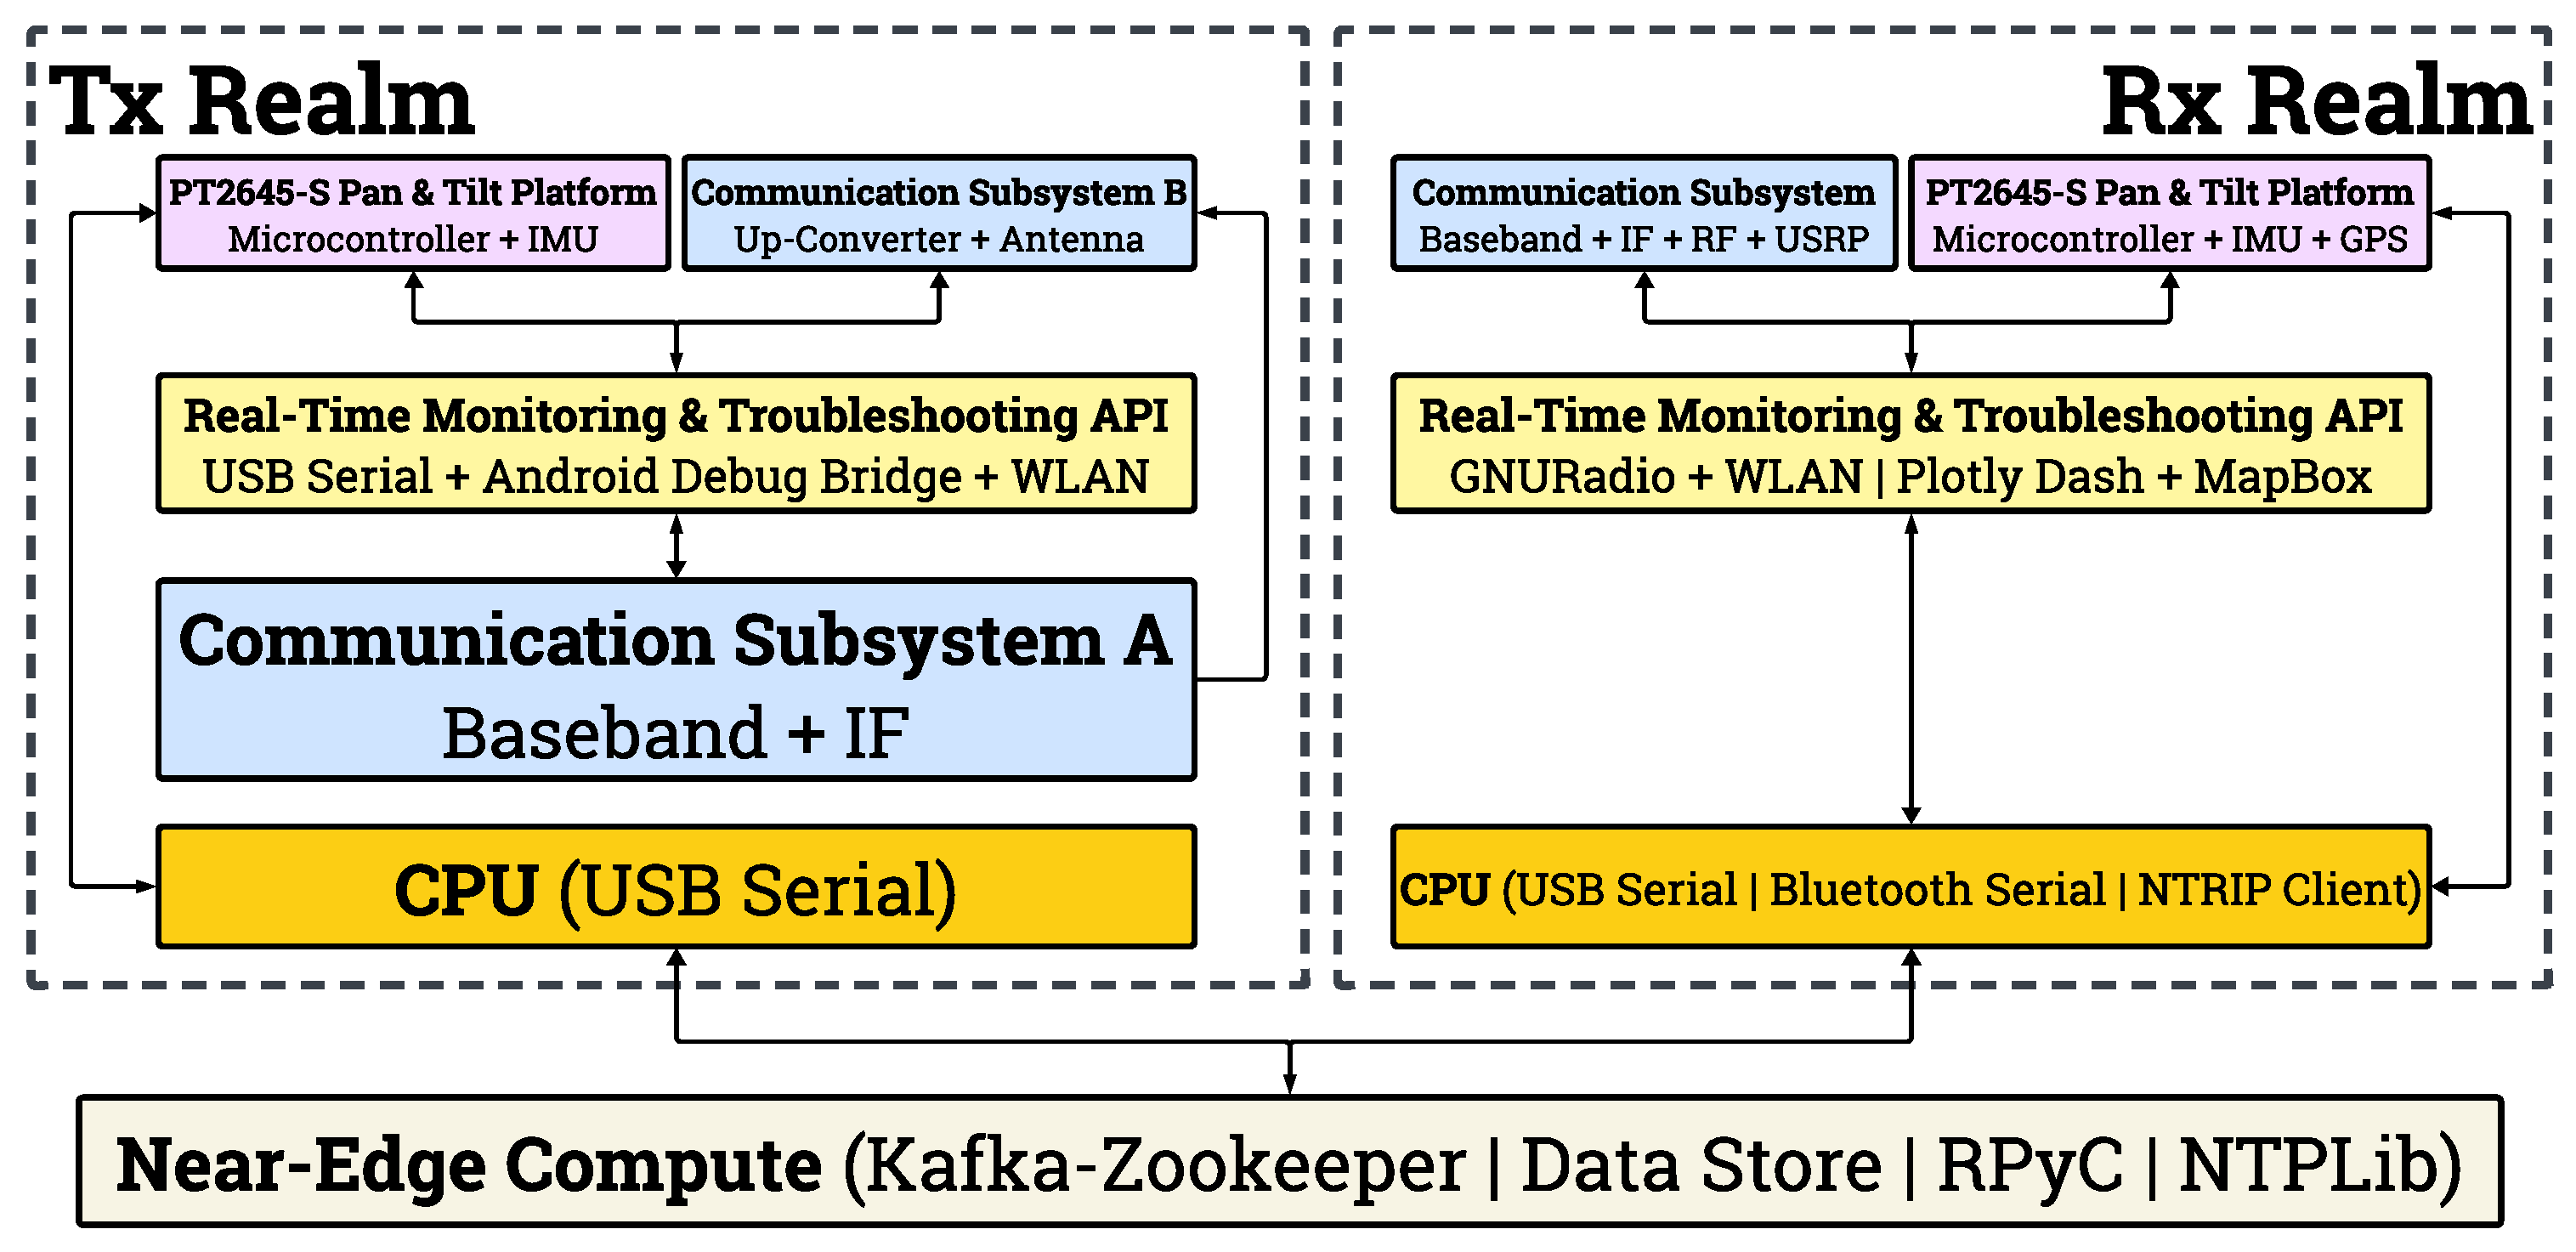
\includegraphics[width=1.0\textwidth]{figs/system_architecture.pdf}
    \vspace{-8mm}
    \caption{The system architecture of our fully-autonomous robotic beam-steering platform with a sliding-correlator channel sounder.}
    \label{F1}
\end{figure*}

\noindent{\textbf{Channel Sounder}}: The measurement system employed a custom broadband sliding-correlator channel sounder at both the Tx and the Rx~\cite{Purdue}, each equipped with a Pseudorandom Noise (PN) sequence generator module producing the required known apriori signal for time-dilated cross-correlation studies, with the Rx module clocked at a slightly lower rate than the Tx; an up-/down-converter to transition between the \SI{2.5}{\giga\hertz} and \SI{28}{\giga\hertz} regimes; a vertically polarized WR-$28$ directional horn antenna; and other commercially available components. This setup is implemented according to the schematics shown in Fig.~\ref{F2a} and Fig.~\ref{F2b}. The operational specifications of the sounder are listed in Table~\ref{T3}, as detailed also in~\cite{Purdue}. As a part of the data-logging operations at the Rx, complex-\SI{64}{} I/Q power delay profiles are recorded onboard an SSD storage drive by a GNURadio sink on a Raspberry Pi SBC via a USRP B$200$mini SDR.

\noindent{\textbf{Alignment \& Tracking}}: First, to enable uninhibited rotational mobility for alignment and tracking in the horizontal and the vertical planes, at both the Tx and the Rx, the WR-$28$ horn antenna is mounted on a PT$2645$-S open-loop pan-and-tilt platform, each driven by a pair of HSR-$2645$CRH continuous rotation servos, with each servo actuating either yaw (horizontal) or pitch (vertical) alignment. These servos are controlled via PWM signals from an ATMega$328$P microcontroller with the angular position feedback provided by a BNO$080$ inertial motion unit. This principal axes positioning subsystem demonstrates an average accuracy of \SI{1.1}{\degree} across all coarse- \& fine-grained yaw and pitch movements. Next, for seamless operations in V$2$X scenarios, this alignment platform is augmented with a geo-positioning subsystem consisting of a UBlox GPS ZED-F$9$P unit (with a GNSS multi-band antenna) wherein the positioning accuracy is enhanced by RTCMv$3.0$ RTK correction streams over NTRIP. Demonstrating an average $3$D accuracy of \SI{17}{\centi\meter}, the relevant data members captured by this geo-positioning unit---namely, the coordinate (latitude, longitude, and ellipsoidal altitude), the horizontal speed \& acceleration, and the heading, are communicated to the microcontroller as NMEA-0183 messages over an I2C serial peripheral bus. A glossary of the acronyms/protocols referenced above is given in Table~\ref{T1}.

Since our measurement system revolves around a decoupled design with the alignment and tracking platform replicated at both the Tx and the Rx, a centralized nerve-center handles asynchronous module registration \& de-registration via RPyC object proxying, global timing synchronization via NTP, and coordination between the Tx and Rx over a fault-tolerant Apache Kafka messaging middleware. With an Apache Zookeeper broker manager serving as a distributed configuration, synchronization, and naming registry service for the Kafka cluster, the samples generated by the principal axes positioning and geo-positioning subsystems are shared over Kafka message queues (known as topics, e.g., "SPAVE\_$28$G\_RX\_GPS\_EVENTS"): the Tx subscribes to the alignment and geo-location messages published by the Rx, and vice-versa, resulting in a scalable event-driven modular architecture. Corroborated both onsite and in the laboratory, this publish-subscribe framework facilitates an average beam-steering response time of \SI{27.8}{\milli\second}, evaluated over ${\approx}$\SI{13000}{} interactions. With system monitoring provided over an Android debug bridge and system troubleshooting enabled via serial communication interfaces, our platform demonstrates remote orchestration capabilities - a critical necessity for mmWave propagation modeling in V$2$X settings. To augment these remote monitoring and troubleshooting features further, a GNURadio Qt GUI time-sink (with dynamic trigger levels) allows for real-time visualization of the recorded power delay profiles over an ad-hoc WLAN with the Raspberry Pi SBC; additionally, via the Plotly Dash and MapBox APIs, the Tx and Rx geo-locations are annotated with their relative alignment accuracies and visualized in real-time for onsite validation of the routes traversed on the NSF POWDER experimental testbed in Salt Lake City, UT.
\begin{figure*} [t]
    \centering
    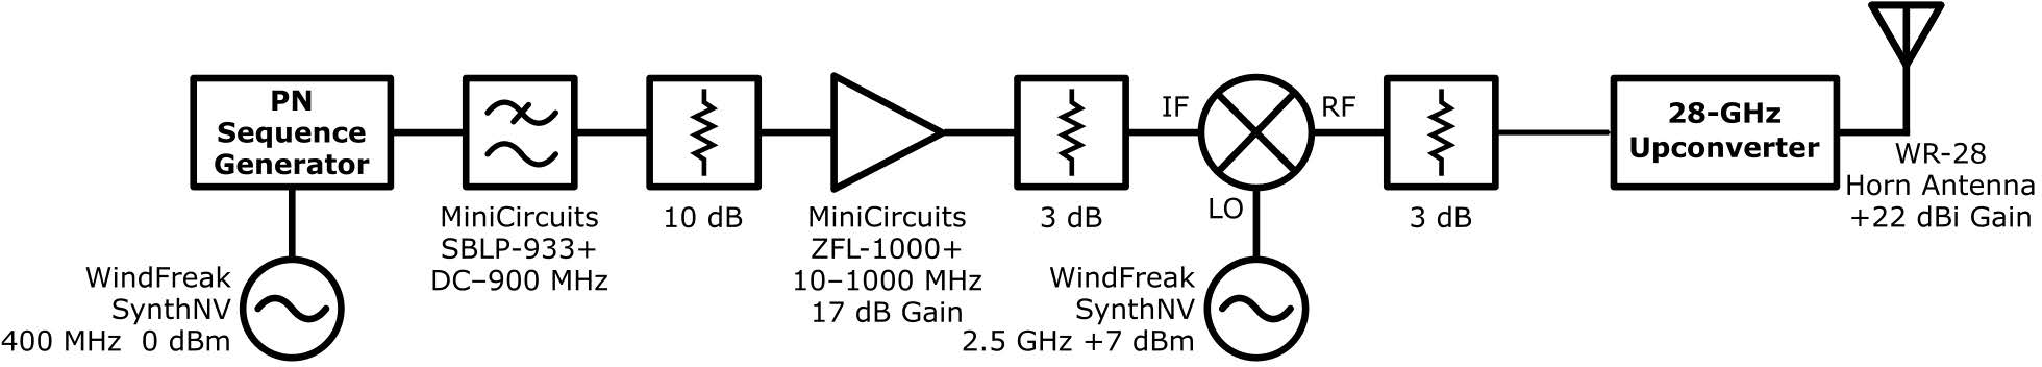
\includegraphics[width=1.0\linewidth]{figs/tx_schematic.pdf}
    \vspace{-6mm}
    \caption{The Tx circuit schematic with an up-converter, a WR-$28$ horn antenna, and other commercially available components.}
    \label{F2a}
    \vspace{-6mm}
\end{figure*}
\begin{figure*} [t]
    \centering
    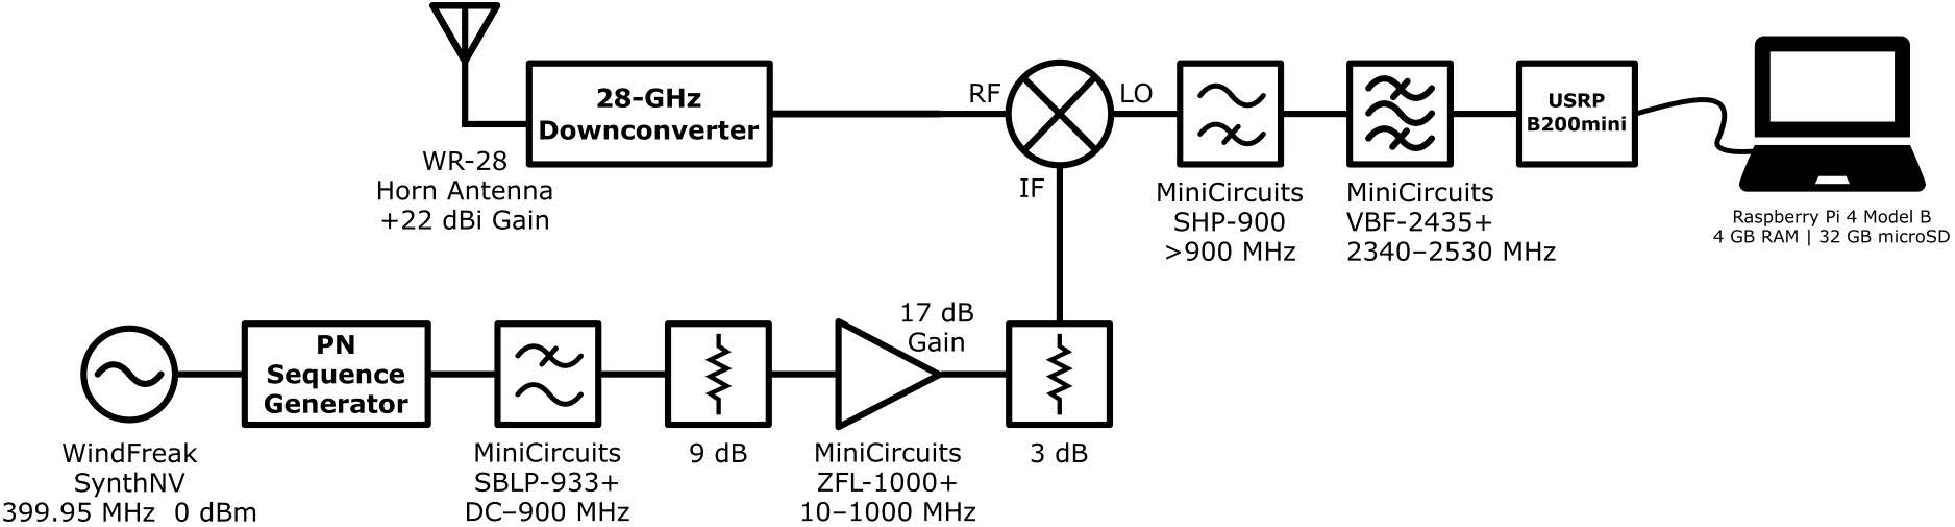
\includegraphics[width=1.0\linewidth]{figs/rx_schematic.pdf}
    \vspace{-6mm}
    \caption{The Rx circuit schematic with a down-converter, a WR-$28$ horn antenna, and other commercially available components.}
    \label{F2b}
\end{figure*}
\renewcommand{\tabcolsep}{6pt}
\begin{table*} [tb]
	\centering
	\scriptsize
	\begin{tabular}{|l||l|}
		\hline
		Carrier Frequency & \SI{28}{\giga\hertz}\\
		\hline
		PN Chip Sequence Length & \SI{2047}{}\\
		\hline
		RF Bandwidth & \SI{800}{\mega\hertz}\\
		\hline
		Tx Chip Rate & \SI{400}{\mega{cps}}\\
		\hline
		Temporal Resolution & \SI{2.5}{\nano\second}\\
		\hline
		Rx Chip Rate & \SI{399.95}{\mega{cps}}\\
		\hline
		Tx Power & \SI{23}{\deci\bel{m}}\\
		\hline
		Tx/Rx Antenna Gain & \SI{22}{\deci\bel{i}}\\
		\hline
		Nominal Tx/Rx Antenna HPBW & \SI{15}{\degree}\\
		\hline
		Measured Tx/Rx Azimuth HPBW & \SI{10.1}{\degree}\\
		\hline
		Measured Tx/Rx Elevation HPBW & \SI{11.5}{\degree}\\
		\hline
		Maximum Measurable Pathloss & \SI{182}{\decibel}\\
		\hline
		GNURadio Sink Center Frequency & \SI{2.5}{\giga\hertz}\\
		\hline
		USRP Gain & \SI{76}{\decibel}\\
		\hline
		USRP Sampling Rate & \SI{2}{\mega{sps}}\\
		\hline
	\end{tabular}
	\vspace{-1mm}
	\caption{The specifications of the sliding-correlator channel sounder used in our measurement campaign on NSF POWDER.}
	\label{T3}
\end{table*}
\vspace{-3mm}

% Measurement campaign description and Data post-processing procedural explanation
\section{Measurements \& Post-Processing}\label{S3}
In this section, we discuss the operations involved in our \SI{28}{\giga\hertz} V$2$X measurement campaign on the NSF POWDER experimental testbed~\cite{POWDER}. First, we describe the system calibration process; next, we outline the onsite system deployment procedure; subsequently, we detail the post-processing steps involved in setting up the power delay profiles recorded at the Rx for pathloss evaluations including the empirical verifications of mmWave UMa ($3$GPP TR$38.901$, ITU-R M$.2135$) and UMi (METIS, mmMAGIC) outdoor pathloss standards~\cite{MacCartneyModelsOverview}, multipath component extraction and parameter estimation via a custom implementation of the SAGE algorithm~\cite{SAGE}, spatial consistency analyses vis-\`{a}-vis distance and alignment accuracy~\cite{SpatialConsistencyOriginal}, shadowing and small-scale fading studies, multipath clustering analyses involving cluster arrival \& decay characteristics and RMS delay- \& direction-spreads, and empirical validations of popular mmWave statistical/parameterized channel models (SV~\cite{SV_Molisch}, QD~\cite{QDC_NIST}, and stochastic~\cite{Indoor60G}).

\noindent{\textbf{Pre-deployment Calibration}}: After the Tx and Rx circuits for the sliding-correlator channel sounder have been implemented as illustrated in Fig.~\ref{F2a} and Fig.~\ref{F2b}, a calibration procedure is carried out onsite to map the power calculated from the power delay profiles recorded by the USRP to reference measured power levels. The process of calibrating the measurement system before deployment ensures accurate Rx power calculations in the presence of imperfect circuit components, e.g., the Commscope LDF$4$-$50$A \SI{0.5}{{"}} coaxial cables employed at the Tx exhibit losses of up to \SI{0.12}{\deci\bel\per\meter} at \SI{2.5}{\giga\hertz}. Under \SI{0}{\deci\bel} and \SI{76}{\deci\bel} USRP gains, using a Keysight variable attenuator, the recorded power delay profiles are processed to determine the calculated power values mapped to their corresponding reference power levels: the results of this procedure are employed in our numerical evaluations detailed in Sec.~\ref{S4} and Sec.~\ref{S5}~\cite{SPAVE_ICC}. We discuss the deployment of our measurement system onsite at the NSF POWDER experimental testbed next.

\noindent{\textbf{NSF POWDER Deployment}}: As described in Sec.~\ref{S2}, our measurement system assembly constitutes an autonomous beam-steering controller replicated at both the Tx and the Rx, their respective sounder circuits, and a centralized nerve center for aggregation (via RPyC), timing synchronization (via NTP), and coordination (via Kafka-Zookeeper). On the NSF POWDER testbed, the nerve center is deployed on a high-availability cluster of four Dell R$740$ compute nodes at the Fort Douglas datacenter, with fault tolerance being a key feature to ensure storage redundancy for the recorded data. As depicted in Fig.~\ref{F3a}, the Tx is mounted on a building rooftop; while, as shown in Fig.~\ref{F3b}, the Rx is mounted on a van (or a push-cart) that is driven (or pushed) along unplanned routes onsite. Remote monitoring and troubleshooting is provided for validation of geo-positioning, alignment, and power delay profile samples. The goal of this measurement campaign was to obtain a reasonably large dataset of site-specific measurements for evaluating the propagation characteristics of \SI{28}{\giga\hertz} signals in vehicular communication settings. Thus, our propagation modeling activities included V$2$I measurements under manual, semi-, and fully-autonomous alignment operations traversing nine routes spanning urban, suburban, and foliage environments. Although our platform is capable of double-directional measurements and facilitates easy scalability to MIMO settings, we focus only on beam-steered measurements in V$2$X scenarios---specifically for spatial decoherence analyses, multipath cluster arrival \& decay evaluations, shadowing investigations, and small-scale fading studies under dynamic blockages.
\begin{figure*}[t]
    \centering
    \begin{subfigure}{0.355\linewidth}
        \centering
        \includegraphics[width=1.0\linewidth]{figs/tx_deployment.pdf}
        \caption{Tx Deployment at Browning}
        \label{F3a}
    \end{subfigure}
    \begin{subfigure}{0.635\linewidth}
        \centering
        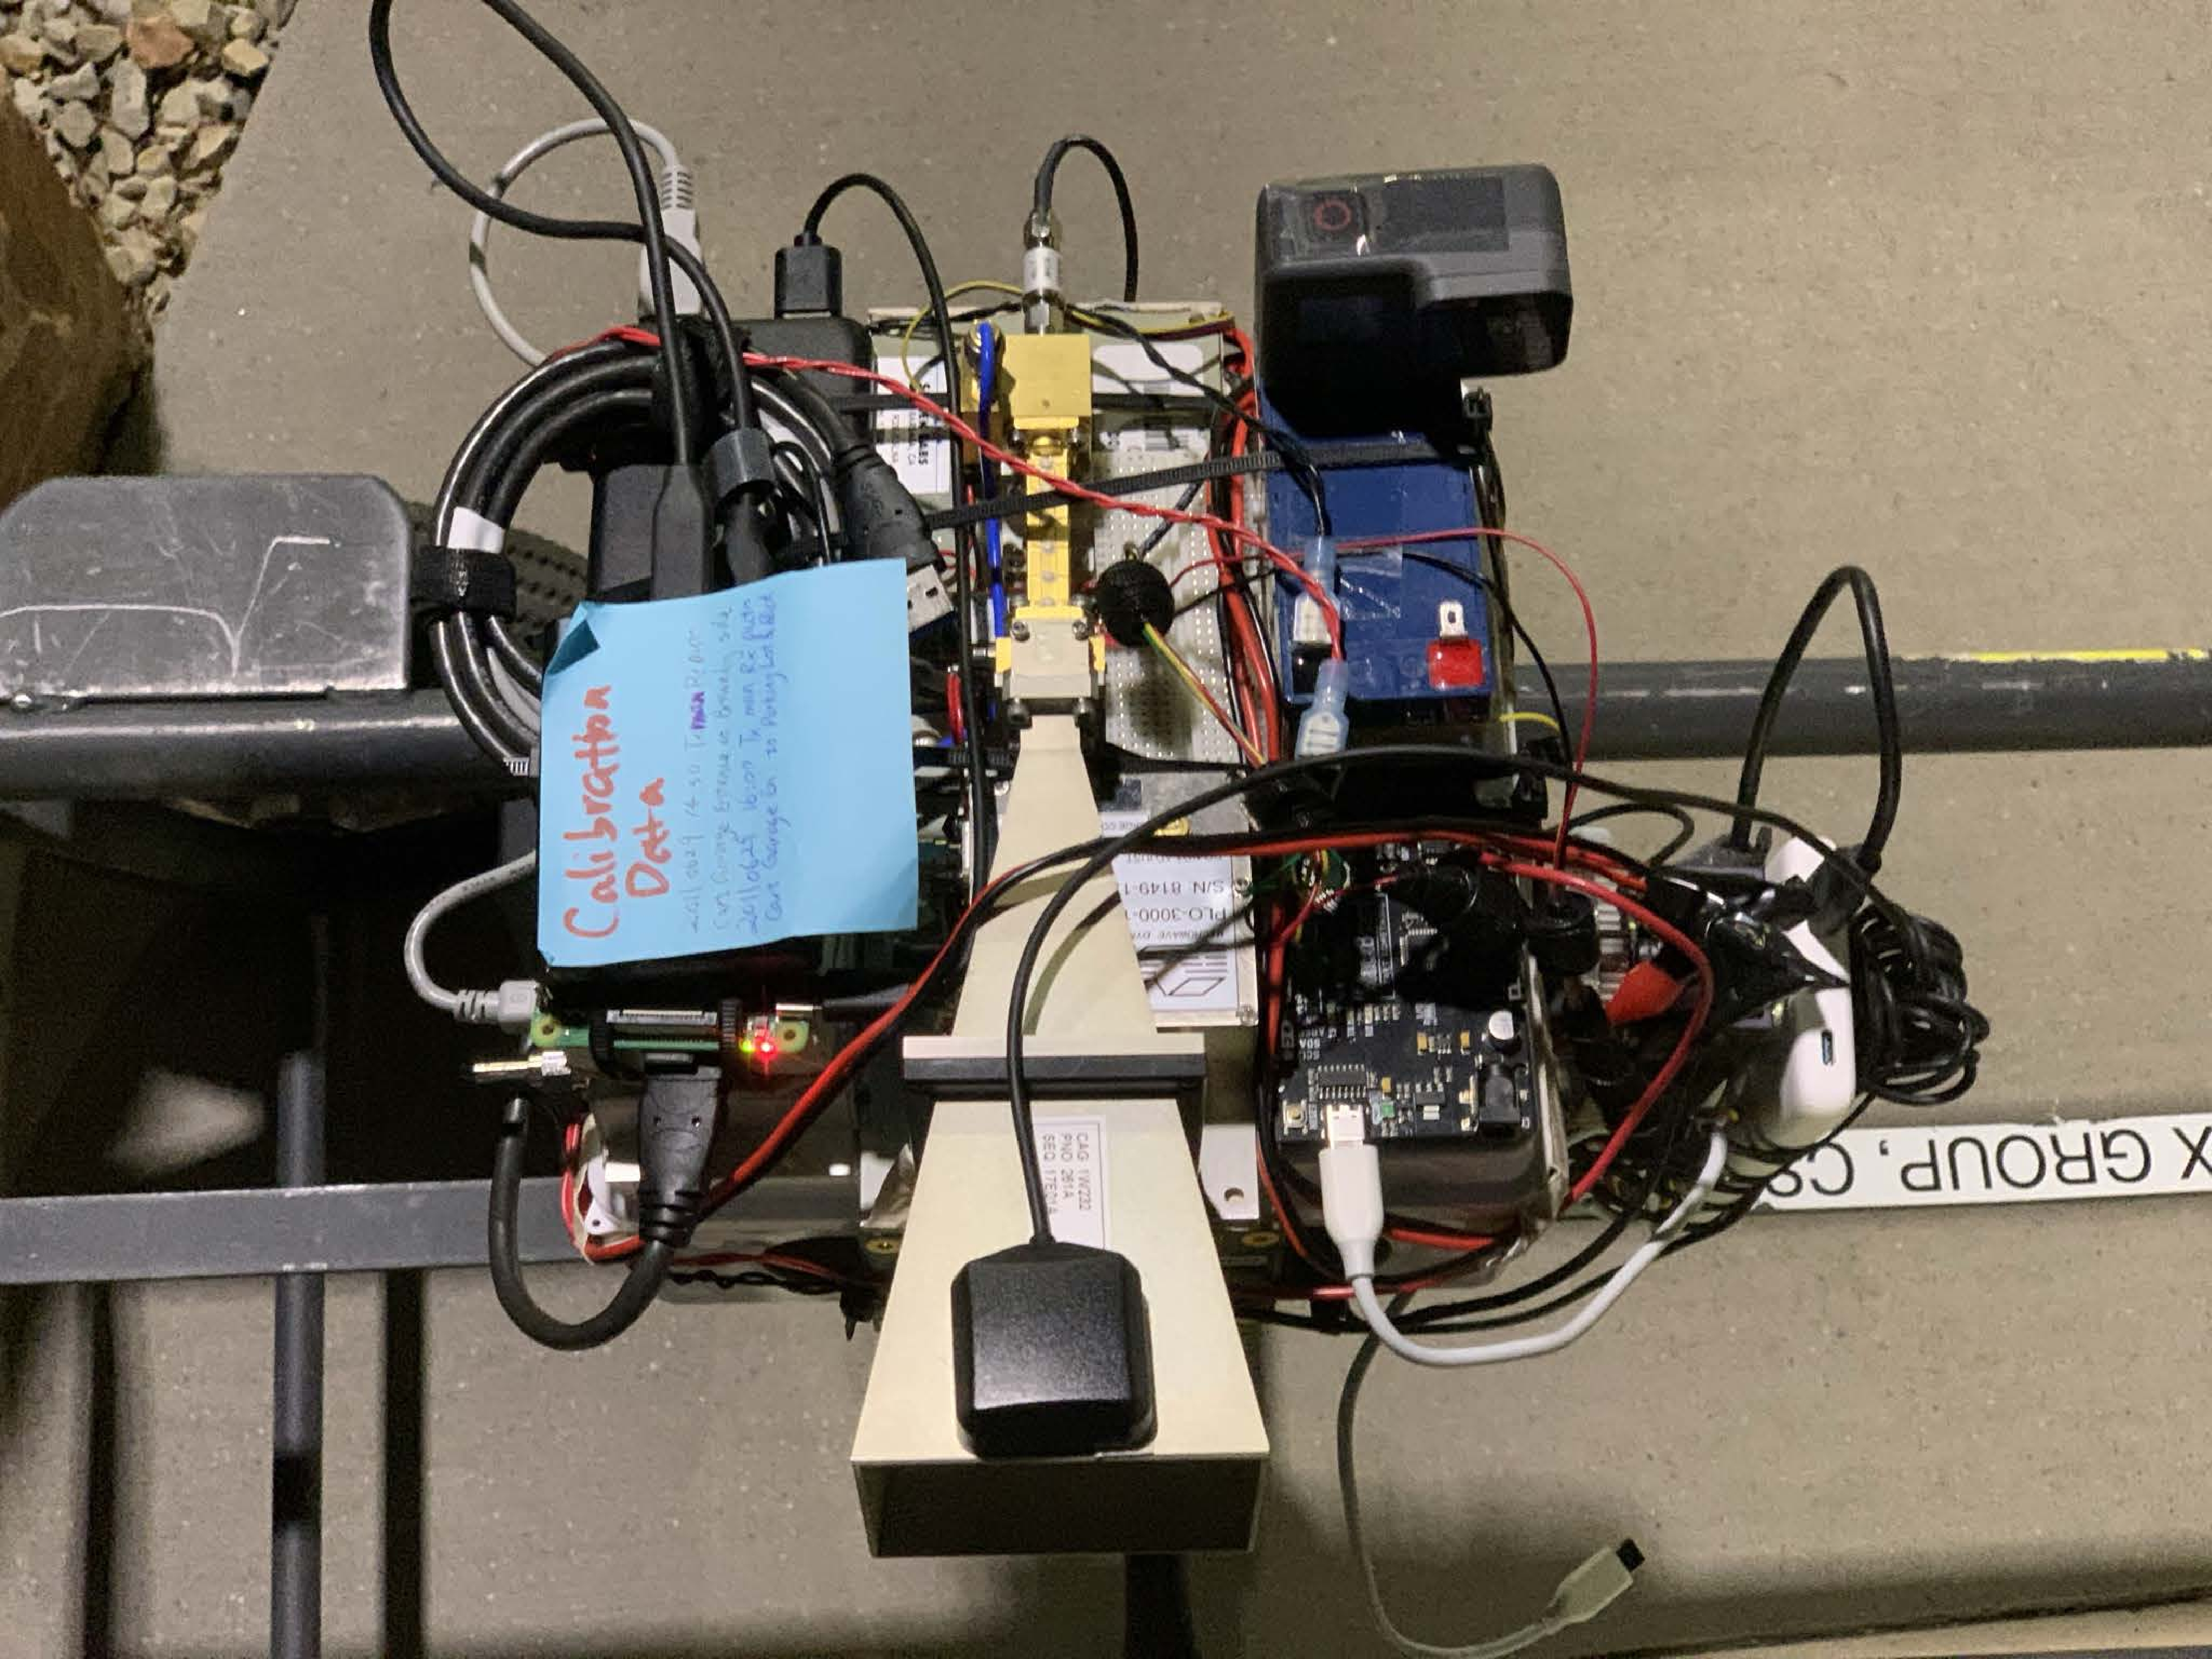
\includegraphics[width=1.0\linewidth]{figs/rx_deployment.pdf}
        \caption{Rx Cart Deployment}
        \label{F3b}
    \end{subfigure}
    \vspace{-8mm}
    \caption{The Tx deployment atop the William Browning building, where the sounder circuits are housed in a climate-controlled enclosure with the antenna mounted on the pan-and-tilt platform (a); and the Rx deployment on a push-cart (or a minivan) (b).}
    \label{F3}
\end{figure*}

\noindent{\textbf{{Post-Processing}}: Using GNURadio utilities, the metadata file corresponding to the route-specific power delay profile records at the Rx is parsed to extract timestamp information, which is then associated with the geo-positioning and alignment logs at both the Tx and the Rx. The samples in each synchronized power delay profile segment undergo pre-filtering via a low-pass filter (SciPy FIR implementation), time-windowing, and noise-elimination (via a custom peak-search and subsequent thresholding mechanism). Coupled with transmission power and antenna gain values, the received power levels obtained from these processed samples allow the visualization of pathloss maps on the Google Maps API (rendered via the Bokeh toolbox), and the evaluation of pathloss behavior as a function of Tx-Rx distance, with validations against the $3$GPP TR$38.901$, ITU-R M$.2135$, METIS, and mmMAGIC standards~\cite{MacCartneyModelsOverview}. Additionally, shadow-fading studies deliver insights on the signal propagation behavior under static terrain/structural blockages; while pathloss versus time visualizations for routes dominant in dynamic blockages (pedestrians and moving/parked vehicles) allow examinations of the small-scale fading properties of mmWave signals (along with comparisons against the D$2$D model~\cite{D2DHumanBlockage}). Next, the SAGE algorithm~\cite{SAGE} is used for multipath component extraction, which facilitates spatial consistency~\cite{SpatialConsistencyOriginal} and multipath clustering evaluations~\cite{Indoor60G}. In particular, under variations in distance and alignment accuracy, we probe signal decoherence patterns via the spatial autocorrelation coefficient~\cite{MacCartneySpatialStatistics}; also, we analyze the multipath clustering characteristics of \SI{28}{\giga\hertz} signals in V$2$X settings vis-\`{a}-vis the inter-arrival times, the decay attributes, and the RMS delay- and direction-spreads. Finally, these studies allow validations of mmWave channel models (SV~\cite{SV_Molisch}, QD~\cite{QDC_NIST}, and stochastic~\cite{Indoor60G}).
\vspace{-3mm}

% Numerical evaluations I: Pathloss studies and Spatial consistency evaluations
\section{Pathloss and Spatial Consistency Evaluations}\label{S4}
In this section, we outline the initial set of results derived from our evaluations on the collected datasets. We first briefly study the radiation patterns of the directional horn antennas and the results of our calibration procedure, both of which are then employed in our ensuing evaluations; next, we analyze the empirical pathloss results attained from our measurements along a diverse set of routes and validate them against popular outdoor pathloss standards~\cite{MacCartneyModelsOverview}; subsequently, we detail our spatial consistency evaluations and examine the signal decoherence behavior under variations in distance and alignment accuracy~\cite{SpatialConsistencyOriginal}; additionally, we outline the insights obtained from our shadow fading investigations under the effects of static geometry-induced losses; and finally, we describe our findings on the small-scale fading attributes of \SI{28}{\giga\hertz} signals in V$2$X applications, in addition to their comparisons with the state-of-the-art D$2$D channel model~\cite{D2DHumanBlockage}. 

\noindent{\textbf{Antenna Patterns \& Calibration}}: Obtained via empirical recordings of the WR-$28$ antenna's operational characteristics, Fig.~\ref{F4} illustrates its normalized measured $2$D radiation patterns along the azimuth and elevation directions: these enable us to compute the gains at specific locations along a route and at specific degrees of alignment, crucial for our subsequent analyses. As evident from these radiation pattern illustrations, the WR-$28$ horn antennas employed in our propagation modeling campaign are highly-directional, thus necessitating the need for an accurate and reliable beam-steering system, particularly in V$2$X measurement scenarios. Furthermore, conducting the pre-deployment calibration procedure as outlined in Sec.~\ref{S3}, we derive a linear relationship between the measured received power levels and their calculated power values corresponding to artificial attenuation injections into the signal path between the Tx and the Rx. This calibration relationship (for both \SI{0}{\deci\bel} and \SI{76}{\deci\bel} USRP gain values) allows us to account for losses introduced into our measurements due to imperfect circuit components: refer to the preliminary manuscript of our research efforts for illustrations and additional details~\cite{SPAVE_ICC}.
\begin{figure*} [t]
    \centering
    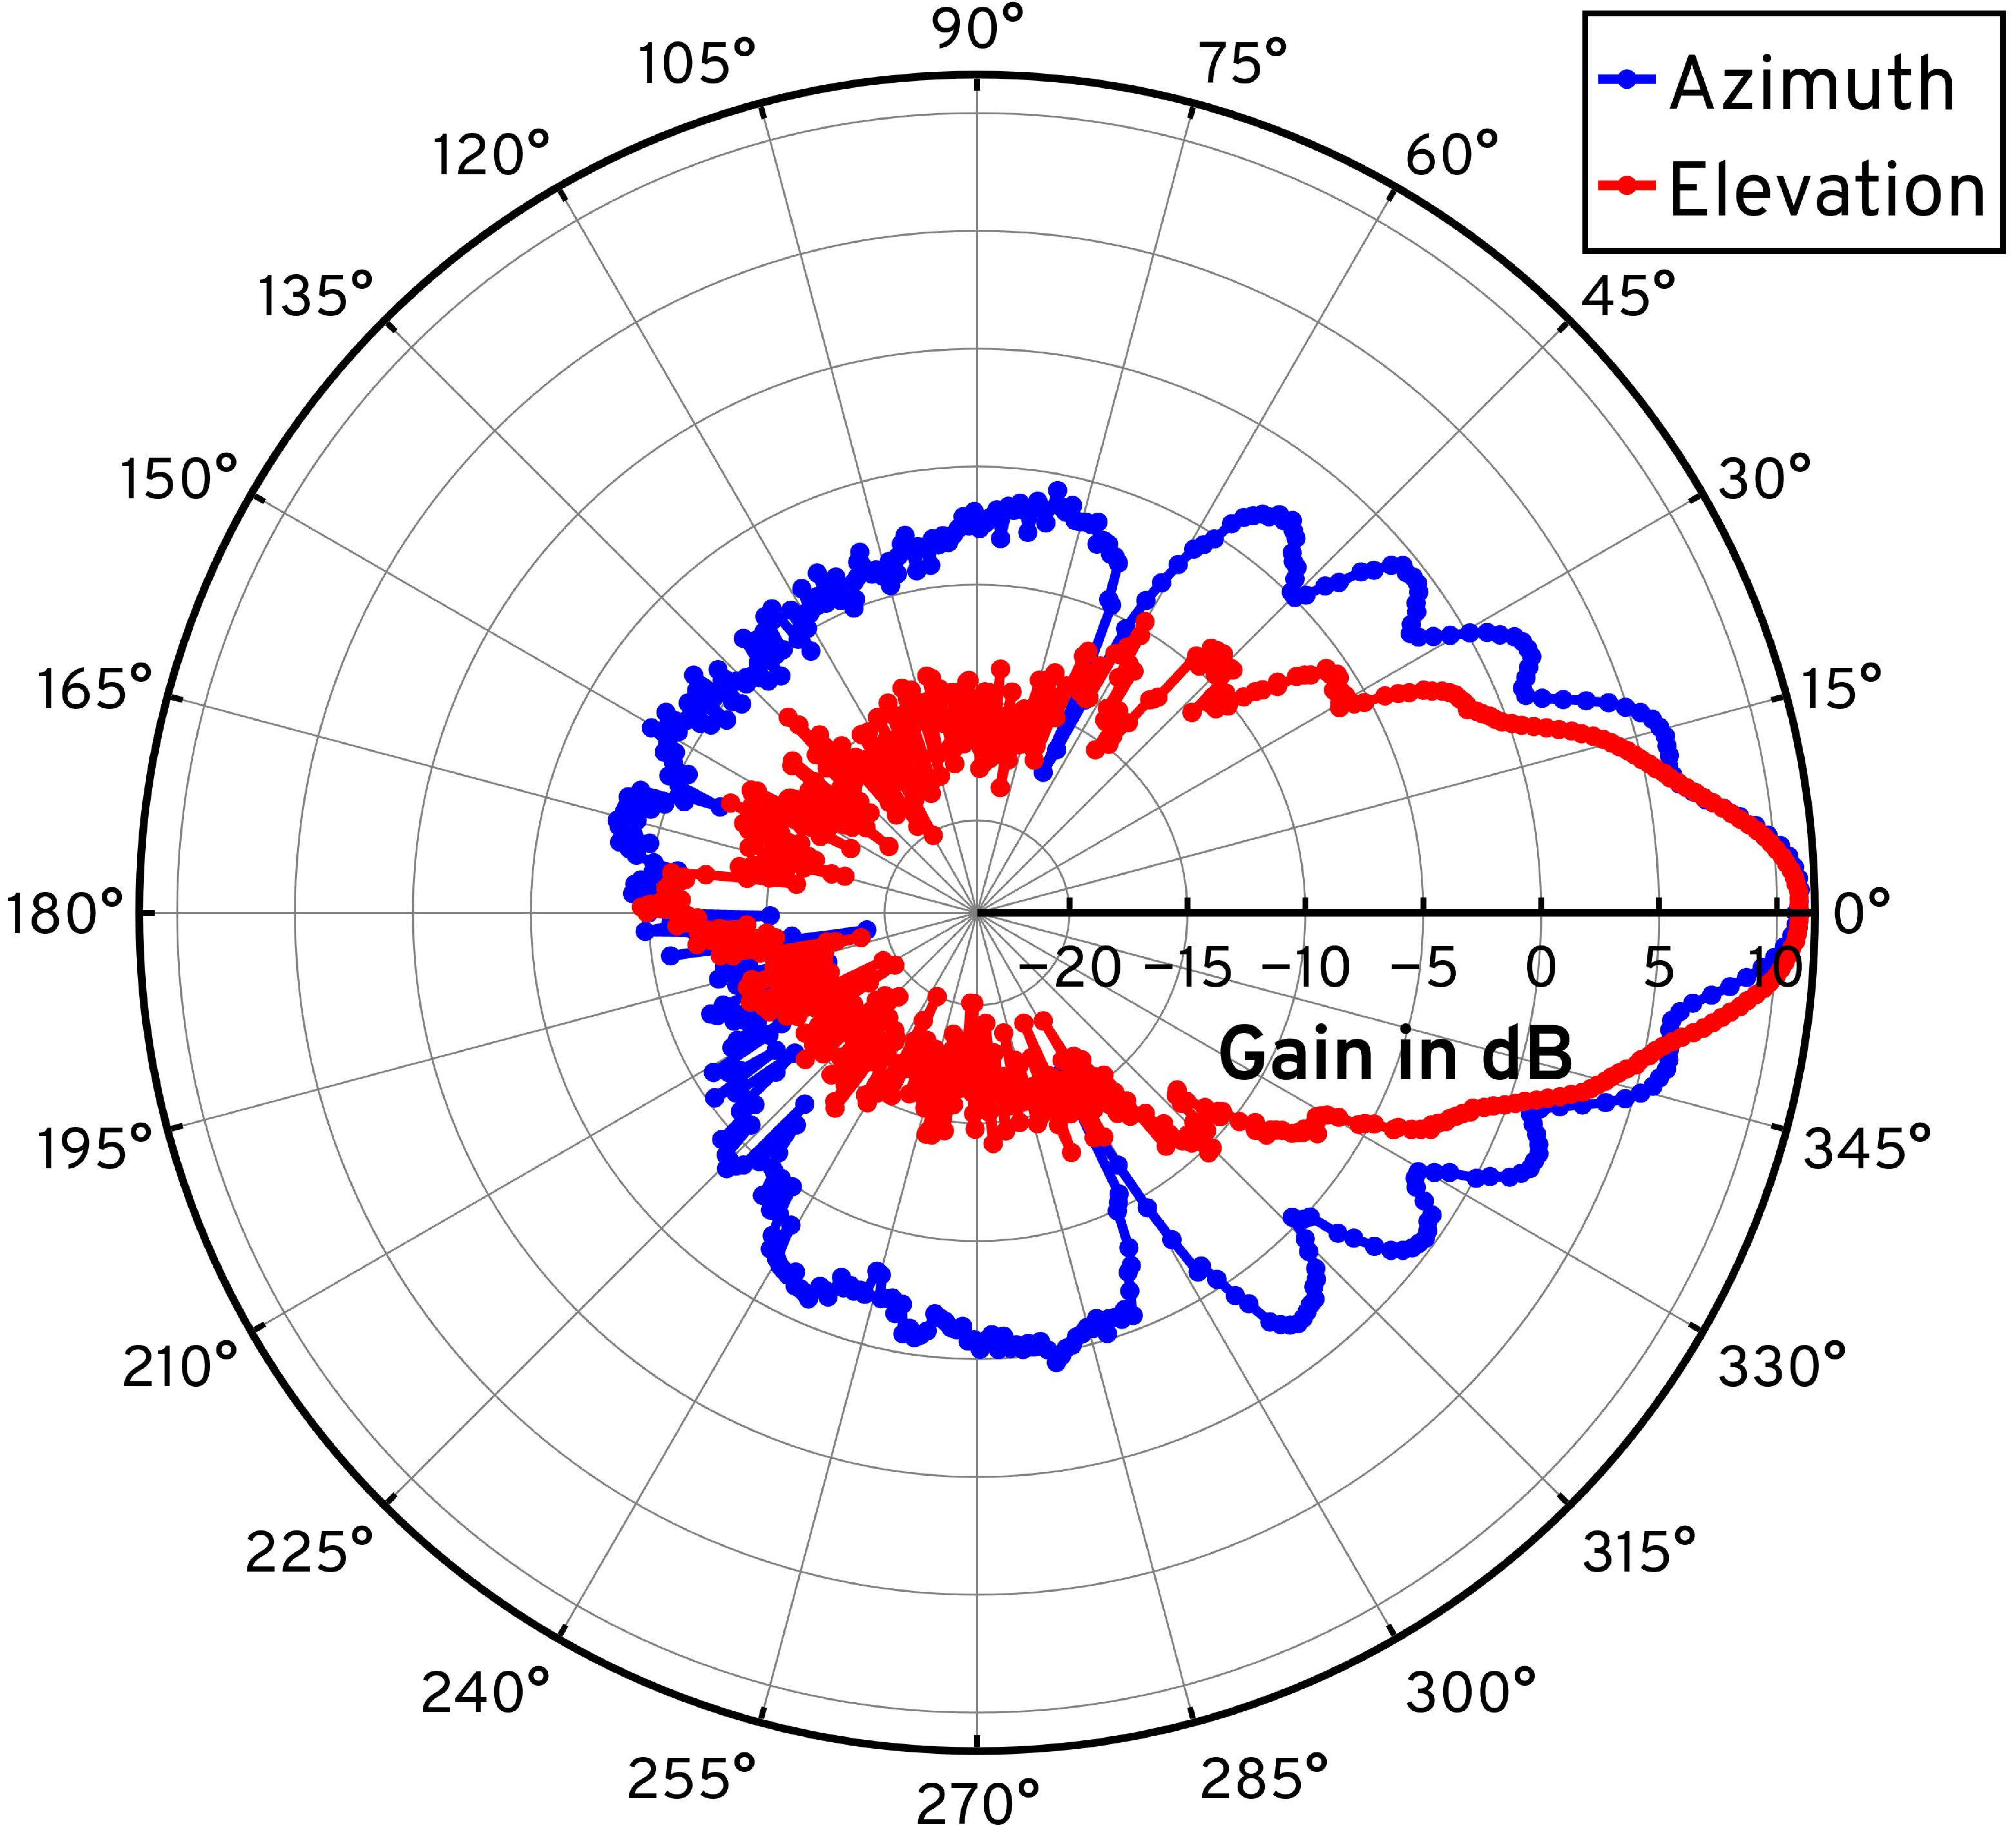
\includegraphics[width=0.55\linewidth]{figs/antenna_patterns.pdf}
    \vspace{-2mm}
    \caption{The normalized measured $2$D radiation patterns along the azimuth and elevation directions for our WR-$28$ horn antennas.}
    \label{F4}
\end{figure*}

\noindent{\textbf{Pathloss Studies}}: Upon post-processing the collected datasets (geo-positioning logs, alignment samples, and power delay profiles) according to the processing operations detailed in Sec.~\ref{S3}, we compute the signal power at the Rx (with calibration offsets); subsequently, knowing the Tx power and the antenna gains, we compute the pathloss experienced at each Rx position around a specific route onsite. Fig.~\ref{F5a} and Fig.~\ref{F5b} depict the pathloss heat-maps (superimposed on Google hybrid maps) for the urban campus routes traversed during our campaign---namely, the route around President's Circle and the route around $100$ S St, respectively. With the Tx affixed atop the William Browning building, for the urban campus route around President's Circle (Fig.~\ref{F5a}), the Rx was mounted on a minivan and driven around onsite, while for the urban campus route around $100$ S St (Fig.~\ref{F5b}), the Rx was mounted on a cart and pushed around onsite. It is evident from these pathloss heatmaps in Fig~\ref{F5a} and Fig.~\ref{F5b} that the received signals along the $100$ S St route (Fig.~\ref{F5b}) as opposed to those along the President's Circle route (Fig.~\ref{F5a}) experience relatively lower pathloss due to their comparatively smaller Tx-Rx distances and smaller Tx-Rx relative velocities (cart vs van). Also, note that in Fig.~\ref{F5b}, since at certain locations, the Rx is hidden behind tall buildings, the obstacle-induced losses (i.e., shadow fading) have a dominant impact on the received signal strength: this is discussed in further detail later in this section. Similarly, Fig.~\ref{F6a} and Fig.~\ref{F6b} depict the pathloss heat-maps (superimposed on Google hybrid maps) of the foliage-dominated route (campus vegetation around the Olpin Union building) and the suburban neighborhood route (around S Wolcott St), respectively. With the Tx affixed atop the William Browning building, for both these routes, the Rx is mounted on a cart and pushed around onsite. Evaluating the differences in received signal power trends between these two routes, we observe that, across similar Tx-Rx distances, the foliage-dominated environment (Fig.~\ref{F6a}) as opposed to the suburban environment with a considerably lower vegetation density (Fig.~\ref{F6b}) presents larger pathloss due to the foliage-induced diffractions introduced into the signal propagation path.
\begin{figure*} [t]
    \centering
    \begin{subfigure}{0.564\linewidth}
        \centering
        \includegraphics[width=1.0\linewidth]{figs/urban_campus_pathloss_1.pdf}
        \caption{Urban Campus (President's Circle)}
        \label{F5a}
    \end{subfigure}
    \begin{subfigure}{0.426\linewidth}
        \centering
        \includegraphics[width=1.0\linewidth]{figs/urban_campus_pathloss_2.pdf}
        \caption{Urban Campus ($100$ S St)}
        \label{F5b}
    \end{subfigure}
    \vspace{-8mm}
    \caption{The pathloss values superimposed on a Google hybrid map for the urban campus routes onsite: President's Circle (the Rx is on a minivan) and $100$ S St (the Rx is on a push-cart). Here, the heat-map color palette dots denote the Rx positions along the route, while the blue diamond represents the fixed Tx location atop the William Browning building.}
    \label{F5}
\end{figure*}

Ensuing these heat-map illustrations of the pathlosses experienced by \SI{28}{\giga\hertz} signals around the various routes traversed onsite, we compare the pathloss versus distance behavior of mmWave signals in our measurement campaign with outdoor micro- and macro-cellular pathloss standards ($3$GPP TR$38.901$, ITU-R M$.2135$, METIS, and mmMAGIC~\cite{MacCartneyModelsOverview}). These popular standards constitute both line-of-sight and non-line-of-sight models, with a Tx height of $h_{\text{Tx}}{\approx}$\SI{25}{\meter} and a Tx-Rx $2$D separation range of \SI{10}{\meter}${\leq}d_{2\text{D}}{\leq}$\SI{5000}{\meter}, which match the deployment specifications of our campaign, making them suitable candidates for empirical validations. In particular, as shown in Fig.~\ref{F7a}, evaluating the pathlosses computed from our collected measurements against these standards for the urban campus (President's Circle and $100$ S St), suburban neighborhood (S Wolcott St), and foliage environment (Olpin Union) routes, we observe that all these pathloss standards fail to accurately capture the pathloss versus log-distance behavior of \SI{28}{\giga\hertz} signals in V$2$X propagation scenarios. Specifically, we notice that, employing a linear-curve fitting procedure (via a floating intercept model) to extrapolate the pathloss values across an extended range of Tx-Rx distances (solid lines for our measurements and dashed lines for the subsequent extrapolation), there is a significant discrepancy between our measurements and the standards in the characteristics of the pathloss across such distances. Therefore, we can conclude that the $3$GPP TR$38.901$, ITU-R M$.2135$, METIS, and mmMAGIC large-scale outdoor pathloss standards require considerable improvements to account for mmWave propagation in V$2$X applications.
\begin{figure*} [t]
    \centering
    \begin{subfigure}{0.5565\linewidth}
        \centering
        \includegraphics[width=1.0\linewidth]{figs/foliage_pathloss.pdf}
        \caption{Foliage Environment (Olpin Union)}
        \label{F6a}
    \end{subfigure}
    \begin{subfigure}{0.4335\linewidth}
        \centering
        \includegraphics[width=1.0\linewidth]{figs/suburban_pathloss.pdf}
        \caption{Suburban Neighborhood (S Wolcott St)}
        \label{F6b}
    \end{subfigure}
    \vspace{-8mm}
    \caption{The pathloss values superimposed on a Google hybrid map for foliage environment (the Rx is on a push-cart) and suburban neighborhood (the Rx is again on a push-cart) routes. Here, the heat-map color palette dots denote the Rx positions along the route, while the blue diamond represents the fixed Tx location atop the William Browning building.}
    \label{F6}
\end{figure*}

\noindent{\textbf{SAGE Algorithm}}: To analyze the multipath propagation characteristics of \SI{28}{\giga\hertz} signals, we employ the SAGE algorithm~\cite{SAGE} to extract the complex attenuation ($\alpha$), delay ($\tau$), Doppler shift ($\nu$), and AoA values ($\phi,\theta$) of the multiple specular paths arriving at the Rx while traversing a particular route onsite. Directly solving for the exact high-resolution maximum likelihood estimate of this parameter vector ($\boldsymbol{\xi}_{l}{=}[\alpha_{l},\tau_{l},\nu_{l},\phi_{l},\theta_{l}]^{\intercal},l{=}1,2,{\dots}$) involves prohibitively large computation times~\cite{SAGE}. Thus, the SAGE algorithm solves for an approximate estimate of $\boldsymbol{\xi}_{l}$ via iterative executions of the E-step which computes the expectation of the log-likelihood given the observations and the previous estimate, and the M-step which computes the current estimate by maximizing over the E-step result. This iterative execution occurs until convergence, i.e., the change in parameter values across consecutive iterations is smaller than a predefined threshold.
\begin{figure*} [t]
    \centering
    \begin{subfigure}{0.49\linewidth}
        \centering
        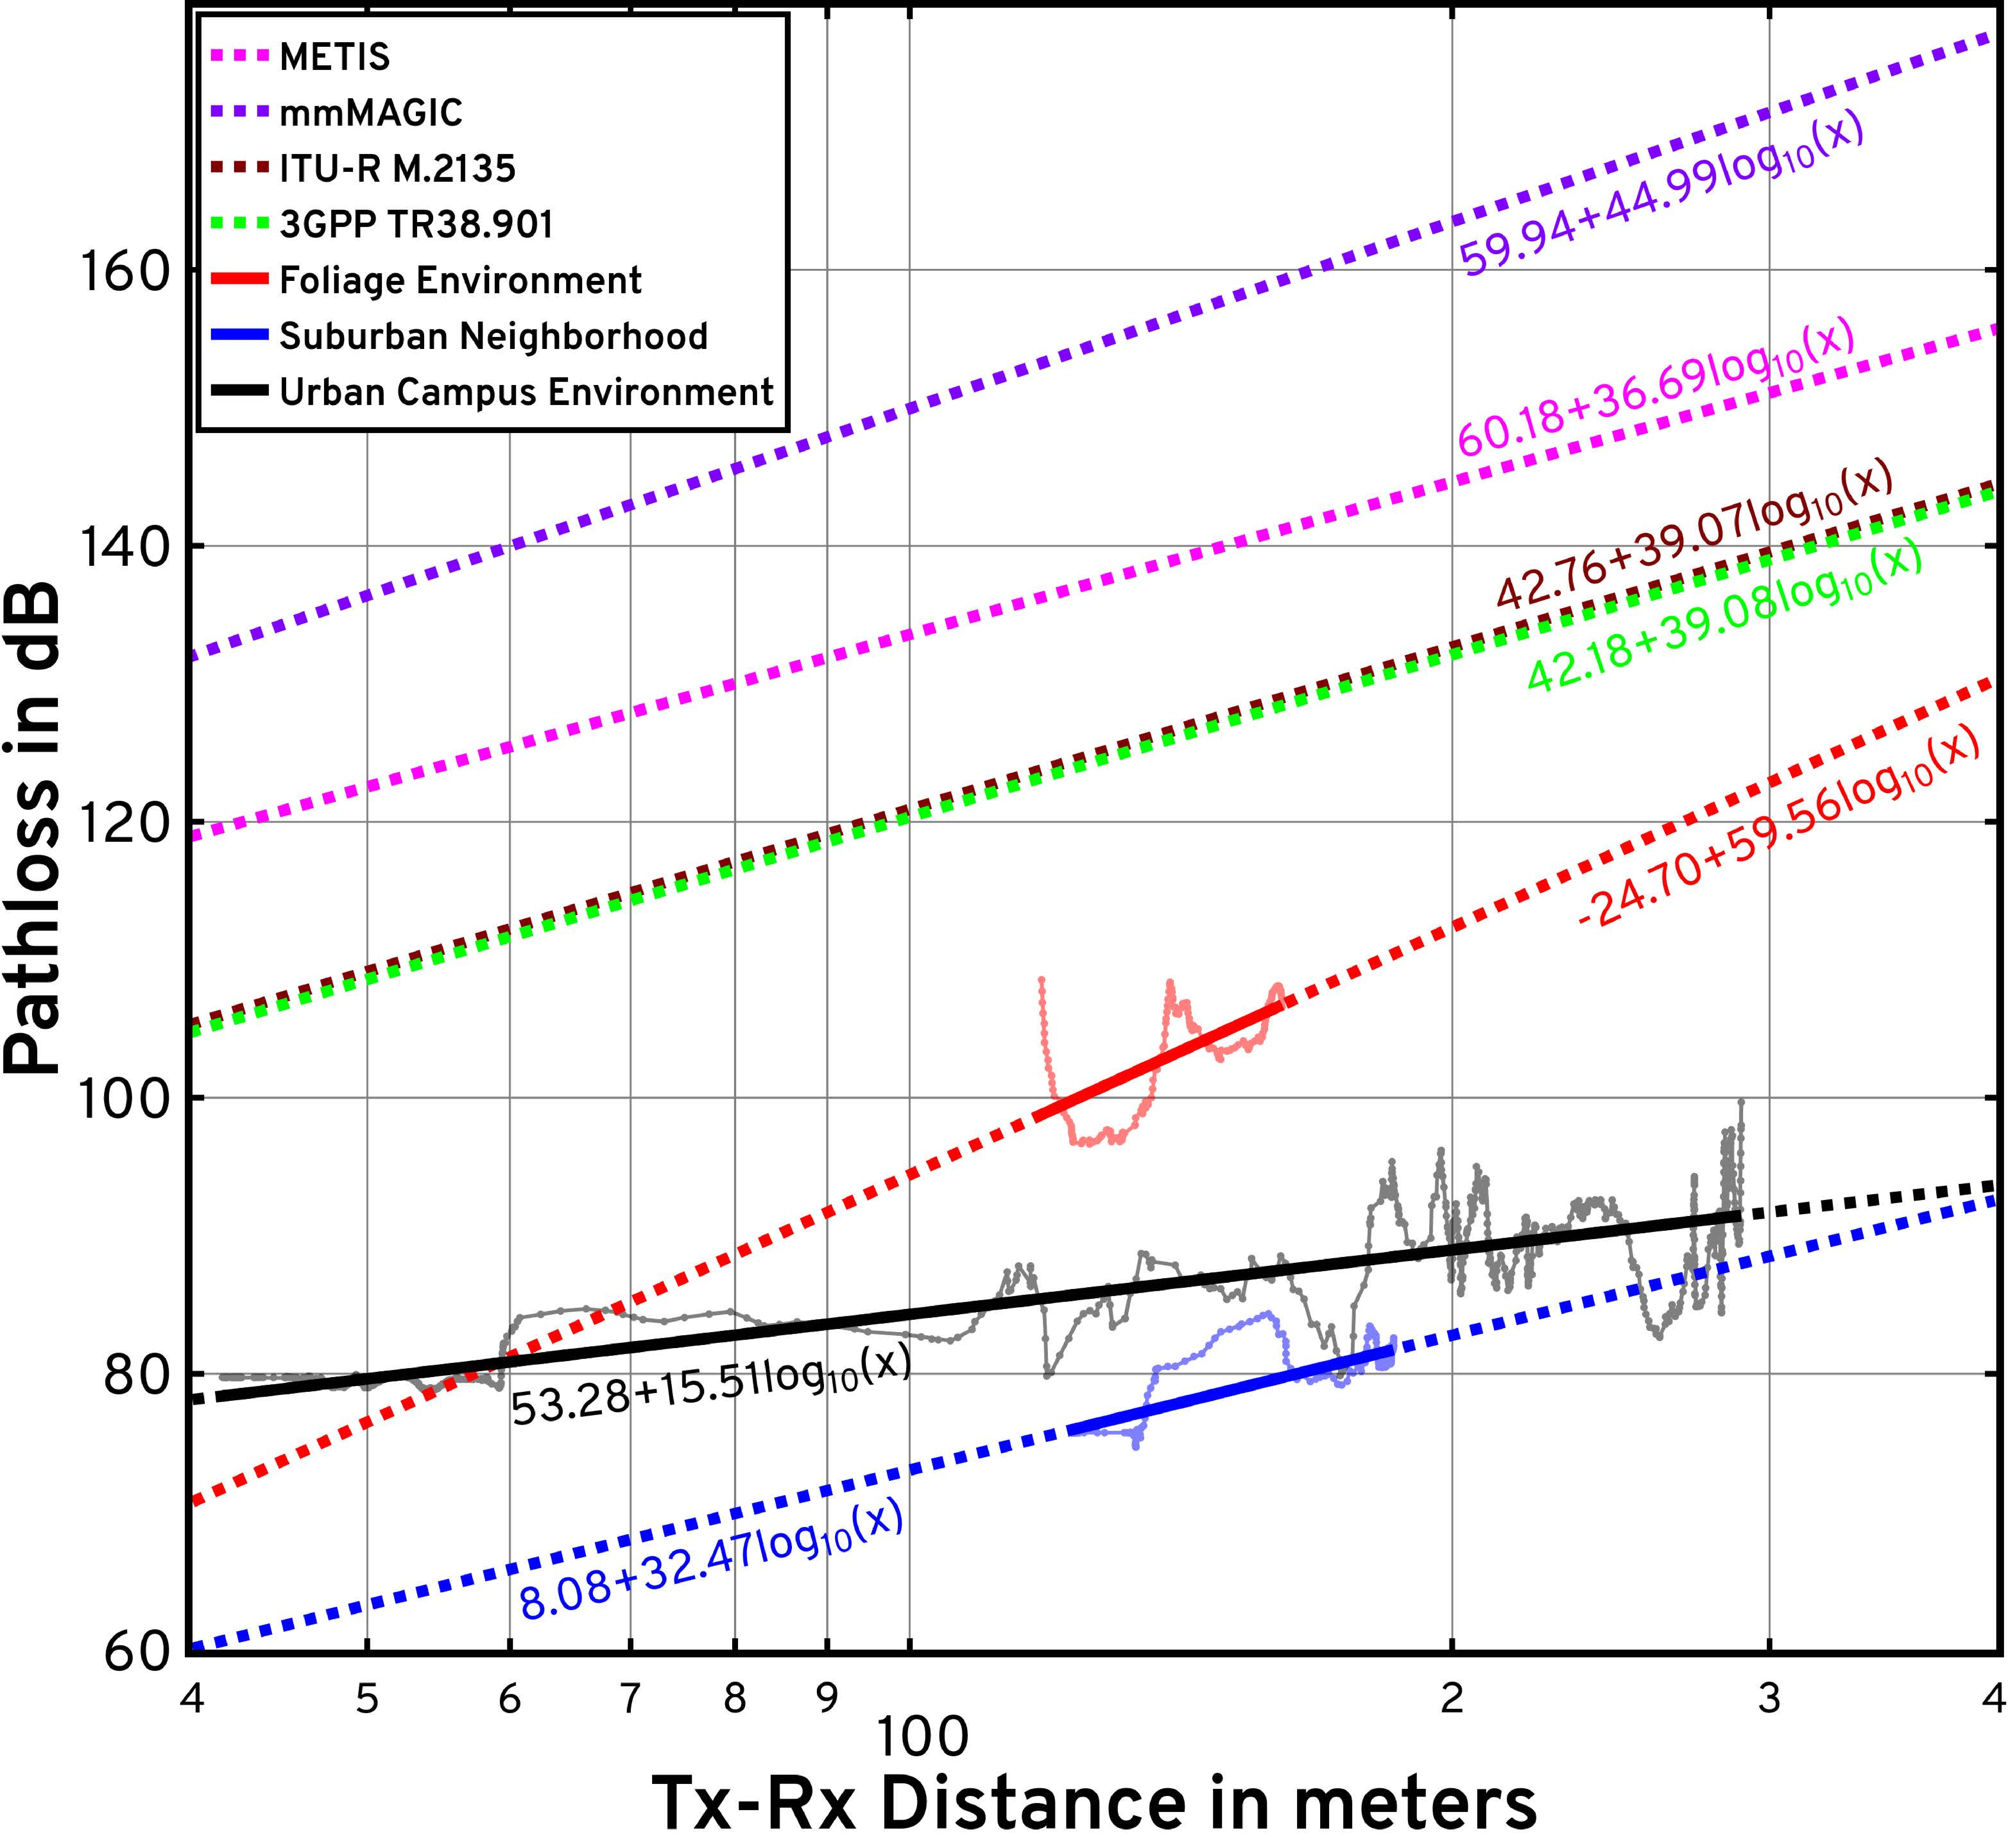
\includegraphics[width=1.0\linewidth]{figs/pathloss_vs_distance.pdf}
        \caption{Pathloss vs Tx-Rx Distance}
        \label{F7a}
    \end{subfigure}
    \begin{subfigure}{0.5\linewidth}
        \centering
        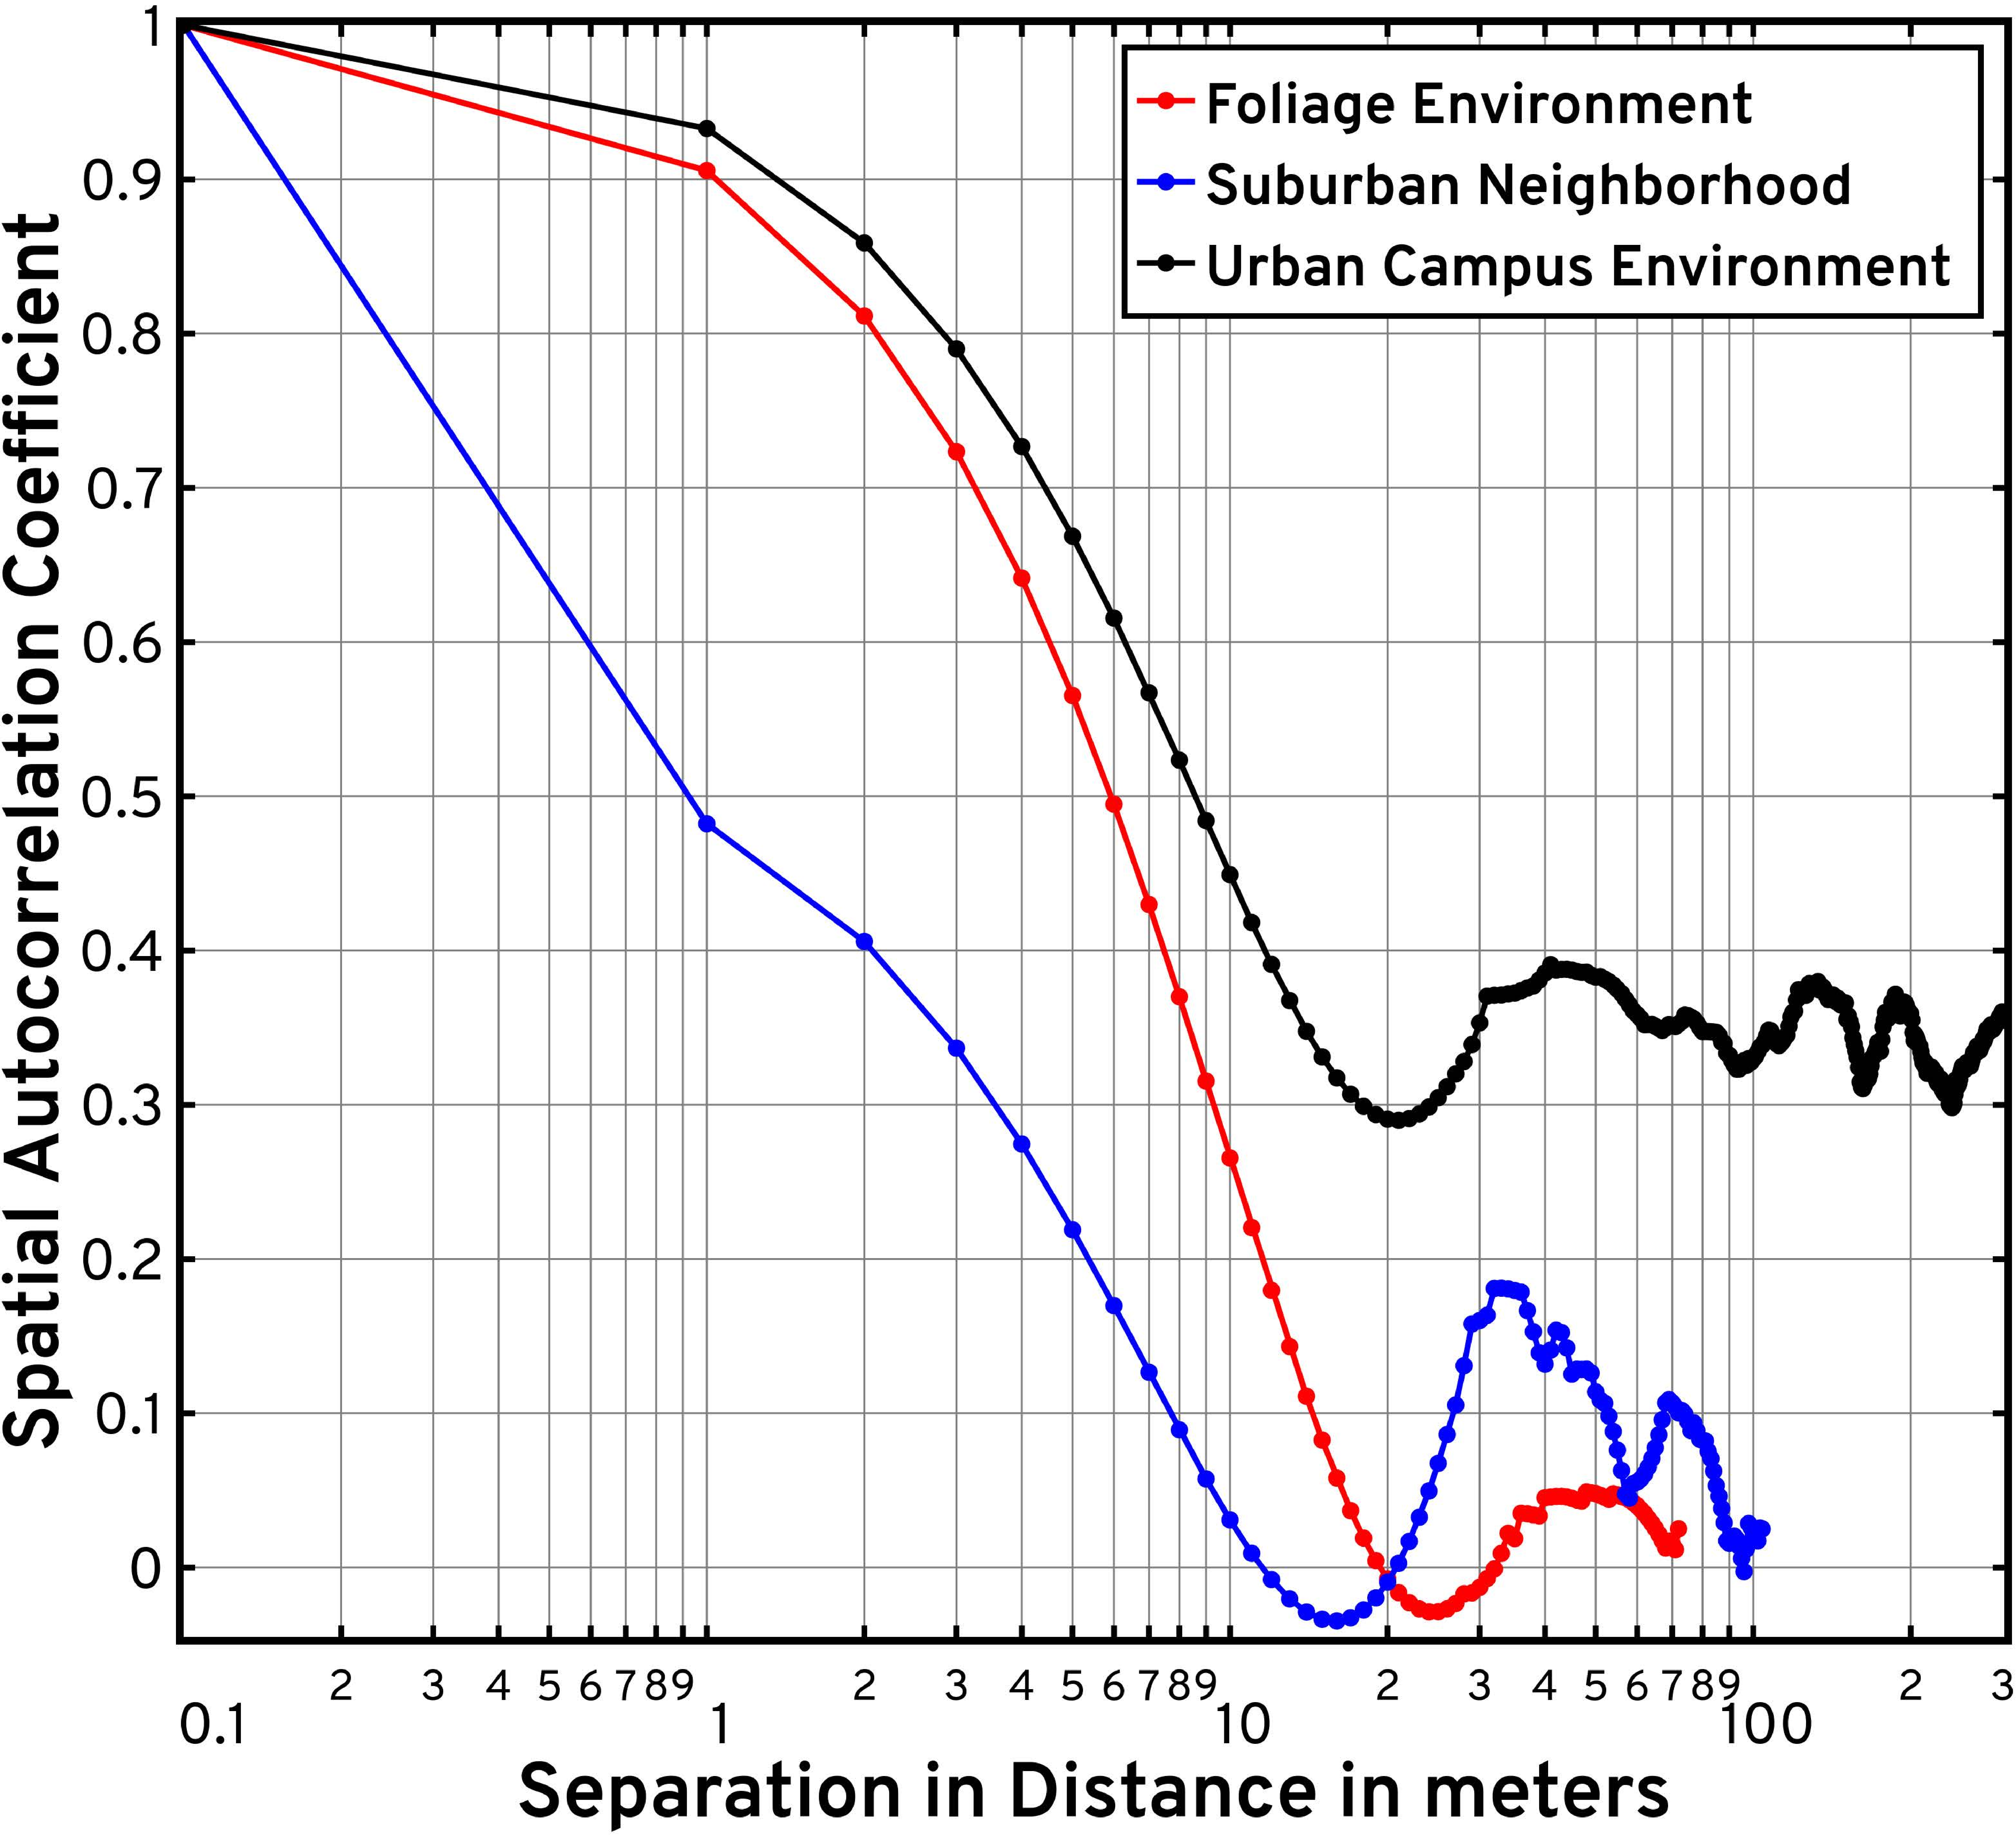
\includegraphics[width=1.0\linewidth]{figs/spatial_consistency_vs_distance.pdf}
        \caption{Spatial Consistency vs Separations in Distance}
        \label{F7b}
    \end{subfigure}
    \vspace{-8mm}
    \caption{An illustration of the measured and extrapolated pathloss (in dB) vs log-distance (in meters) behavior of mmWave signals in V$2$X settings, and their comparisons against the $3$GPP TR$38.901$, ITU-R M.$2135$, METIS, and mmMAGIC standards---with the solid lines denoting our measurements and the dashed lines denoting the corresponding fitted models (a); and a plot depicting the variations in the spatial autocorrelation coefficient under separations in distance (b), i.e., $\rho(\Delta d)$ vs log-distance in meters.}
    \label{F7}
\end{figure*}

\noindent{\textbf{Spatial Consistency}}: In this subsection, to study the spatial decoherence behavior of \SI{28}{\giga\hertz} signals in V$2$X scenarios, we evaluate the spatial autocorrelation coefficient along specific Rx routes under the effects of separations in distance and alignment accuracy. Herein, we first describe the mathematical modeling underlying the computation of the spatial autocorrelation coefficient, after which we outline the insights gained from our results on the decorrelation characteristics of \SI{28}{\giga\hertz} signals in V$2$X settings under distance and alignment accuracy effects.

The small-scale spatial autocorrelation coefficient is a metric to characterize the coherence between the voltage amplitudes of received signals across variations in distances and alignment accuracies. With $\mathcal{I} \triangleq \{1,2,{\dots},I\}$ as the index set, we define a route in our measurement campaign as a set of $4$-tuples, i.e., $\mathcal{R} \triangleq \{\mathcal{T}_{i} \triangleq \left(\mathbf{x}_{i}, \mathbf{y}_{i}, \phi_{i}, \mathcal{M}_{i}\right) \suchthat i \in \mathcal{I}\}$, where $\mathbf{x}_{i}$ denotes the $3$D position vector of the Rx, $\mathbf{y}_{i}$ denotes the $3$D position vector of the Tx, and $\phi_{i}$ denotes the accuracy of alignment between the Tx and Rx horn antennas (i.e., deviation from perfect alignment). Let $\mathcal{J}_{i} \triangleq \{1,2,{\dots},J_{i}\}$ represent the index set for the collection of measurements obtained at the route configuration index $i \in \mathcal{I}$; therefore, the corresponding set of measurements is defined as $\mathcal{M}_{i} \triangleq \{\mathbf{m}_{i,j} \suchthat j \in \mathcal{J}_{i}\}$. As detailed in Sec.~\ref{S3}, each vector of received samples $\mathbf{m}_{i,j}$ undergoes processing via pre-filtering, time-windowing, and noise elimination (peak-search and thresholding); subsequently, with propagation delay bins $\boldsymbol{\tau} \triangleq \{\tau_{1},\tau_{2},{\dots},\tau_{L}\}$ (e.g., $1$ ns to $1000$ ns quantization), we extract the amplitudes of the Multi-Path Components (MPCs) at these delay bins using the SAGE algorithm~\cite{SAGE}, i.e., $\forall i \in \mathcal{I}$, we define the corresponding local set of MPC amplitudes across all delay bins as $\tilde{\mathcal{M}}_{i} \triangleq \left\{\Big[A_{i,j}(\tau_{1}), A_{i,j}(\tau_{2}), \dots, A_{i,j}(\tau_{L})\Big]^{\mathsf{T}} \suchthat j \in \mathcal{J}_{i}\right\}$.

With the Tx fixed ($\mathbf{y}_{i} = \mathbf{y}, \forall i \in \mathcal{I}$), we define the following two sets as evaluation conditions to compute the spatial autocorrelation coefficient~\cite{MacCartneySpatialStatistics} under variations in their corresponding separation variables, i.e., separation in distance $\Delta d$ and separation in alignment accuracy $\Delta \phi$:
\begin{align}\label{E}
    \mathcal{I}(\Delta d) &\triangleq \left\{(i,i') \in \binom{\mathcal{I}}{2}: \norm{\mathbf{x}_{i} - \mathbf{x}_{i'}} = \Delta d, \phi_{i} = \phi_{i'}\right\};\\
    \mathcal{I}(\Delta \phi) &\triangleq \left\{(i,i') \in \binom{\mathcal{I}}{2}: \mathbf{x}_{i} = \mathbf{x}_{i'}, \abs{\phi_{i} - \phi_{i'}} = \Delta \phi\right\}\label{Ea};
\end{align}
where $\mathcal{I}(\Delta d)$ and $\mathcal{I}(\Delta \phi)$ denote the sets employed to compute the spatial autocorrelation coefficient under variations in distance and alignment accuracy, respectively. Here, to ensure that our resultant spatial consistency analyses capture the effects of distance only, the constituent route index pairs in $\mathcal{I}(\Delta d)$ should be separated by a distance of $\Delta d$ ($\norm{\mathbf{x}_{i}{-}\mathbf{x}_{i'}}{=}\Delta d$) while having the same alignment accuracy ($\phi_{i}{=}\phi_{i'}$). Similarly, the definition of $\mathcal{I}(\Delta \phi)$ ensures that our analyses accurately captures the effects of alignment accuracy only by enforcing equal distance ($\mathbf{x}_{i}{=}\mathbf{x}_{i'}$) and $\Delta \phi$ separation in alignment accuracy ($\abs{\phi_{i}{-}\phi_{i'}}{=}\Delta \phi$) for the constituent route index pairs.
\begin{figure*} [t]
    \centering
    \begin{subfigure}{0.4925\linewidth}
        \centering
        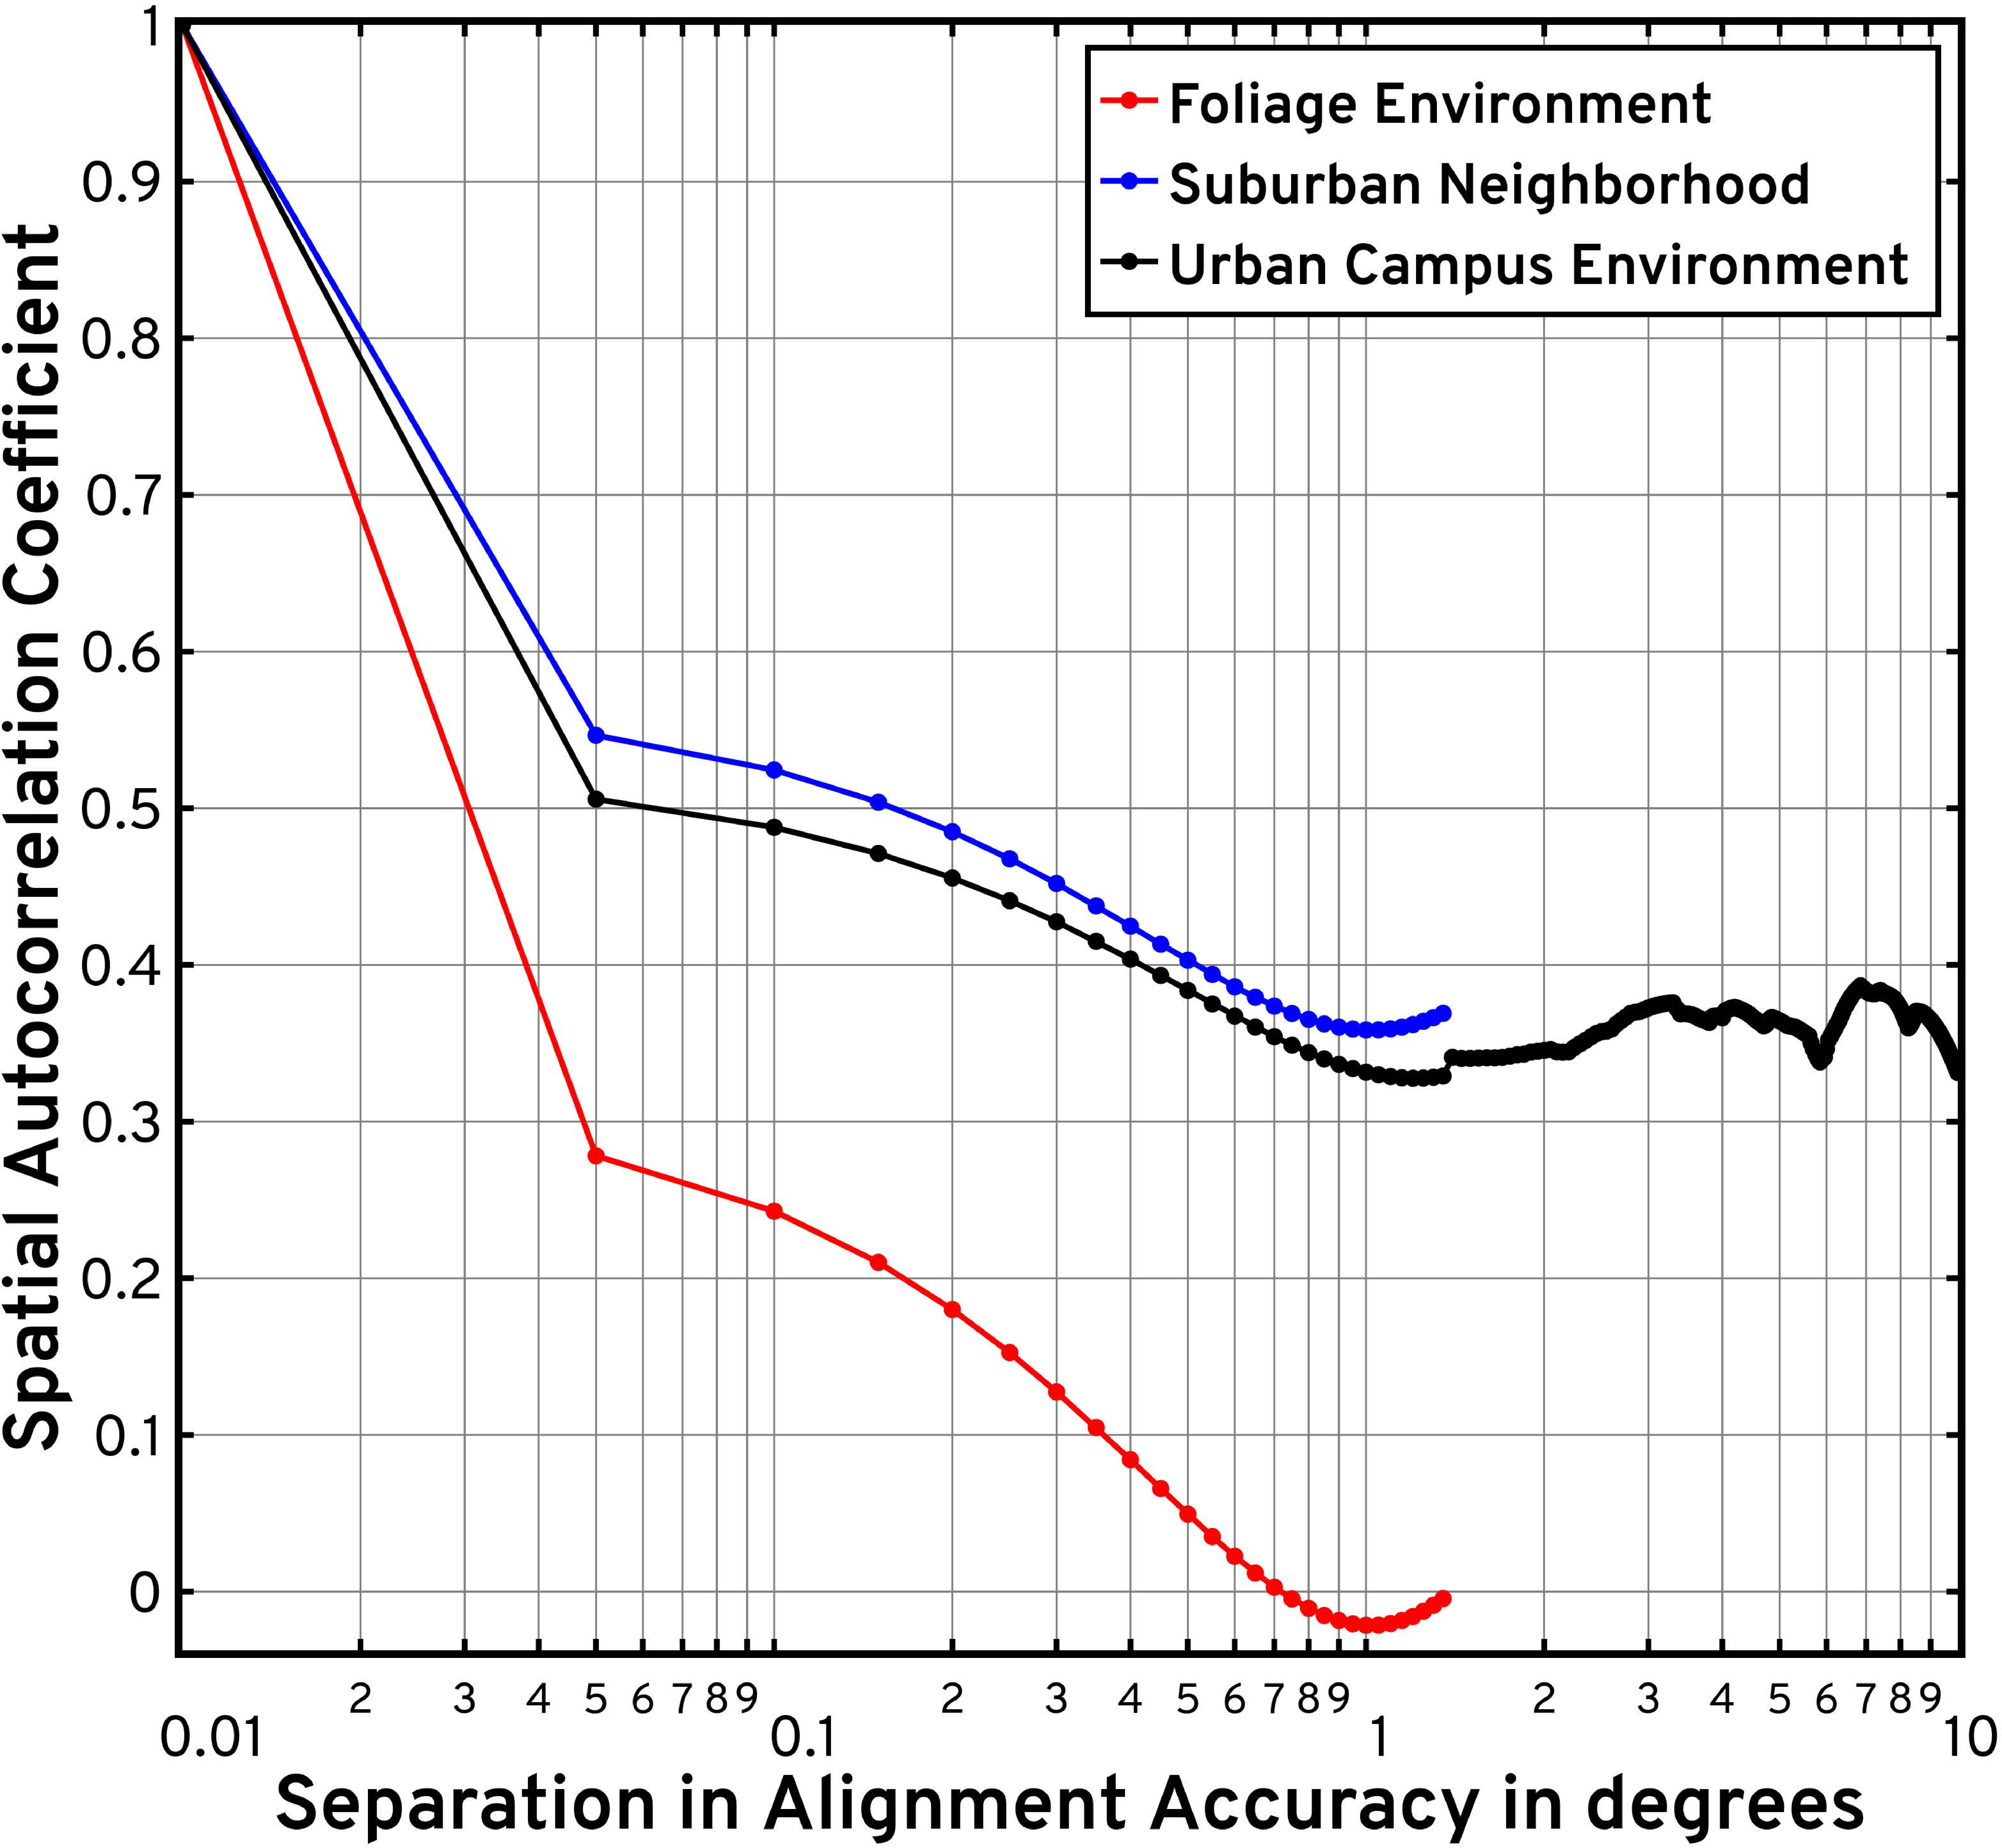
\includegraphics[width=1.0\linewidth]{figs/spatial_consistency_vs_alignment_accuracy.pdf}
        \caption{Spatial Consistency vs Separations in Tx-Rx Alignment Accuracy}
        \label{F8a}
    \end{subfigure}
    \begin{subfigure}{0.4975\linewidth}
        \centering
        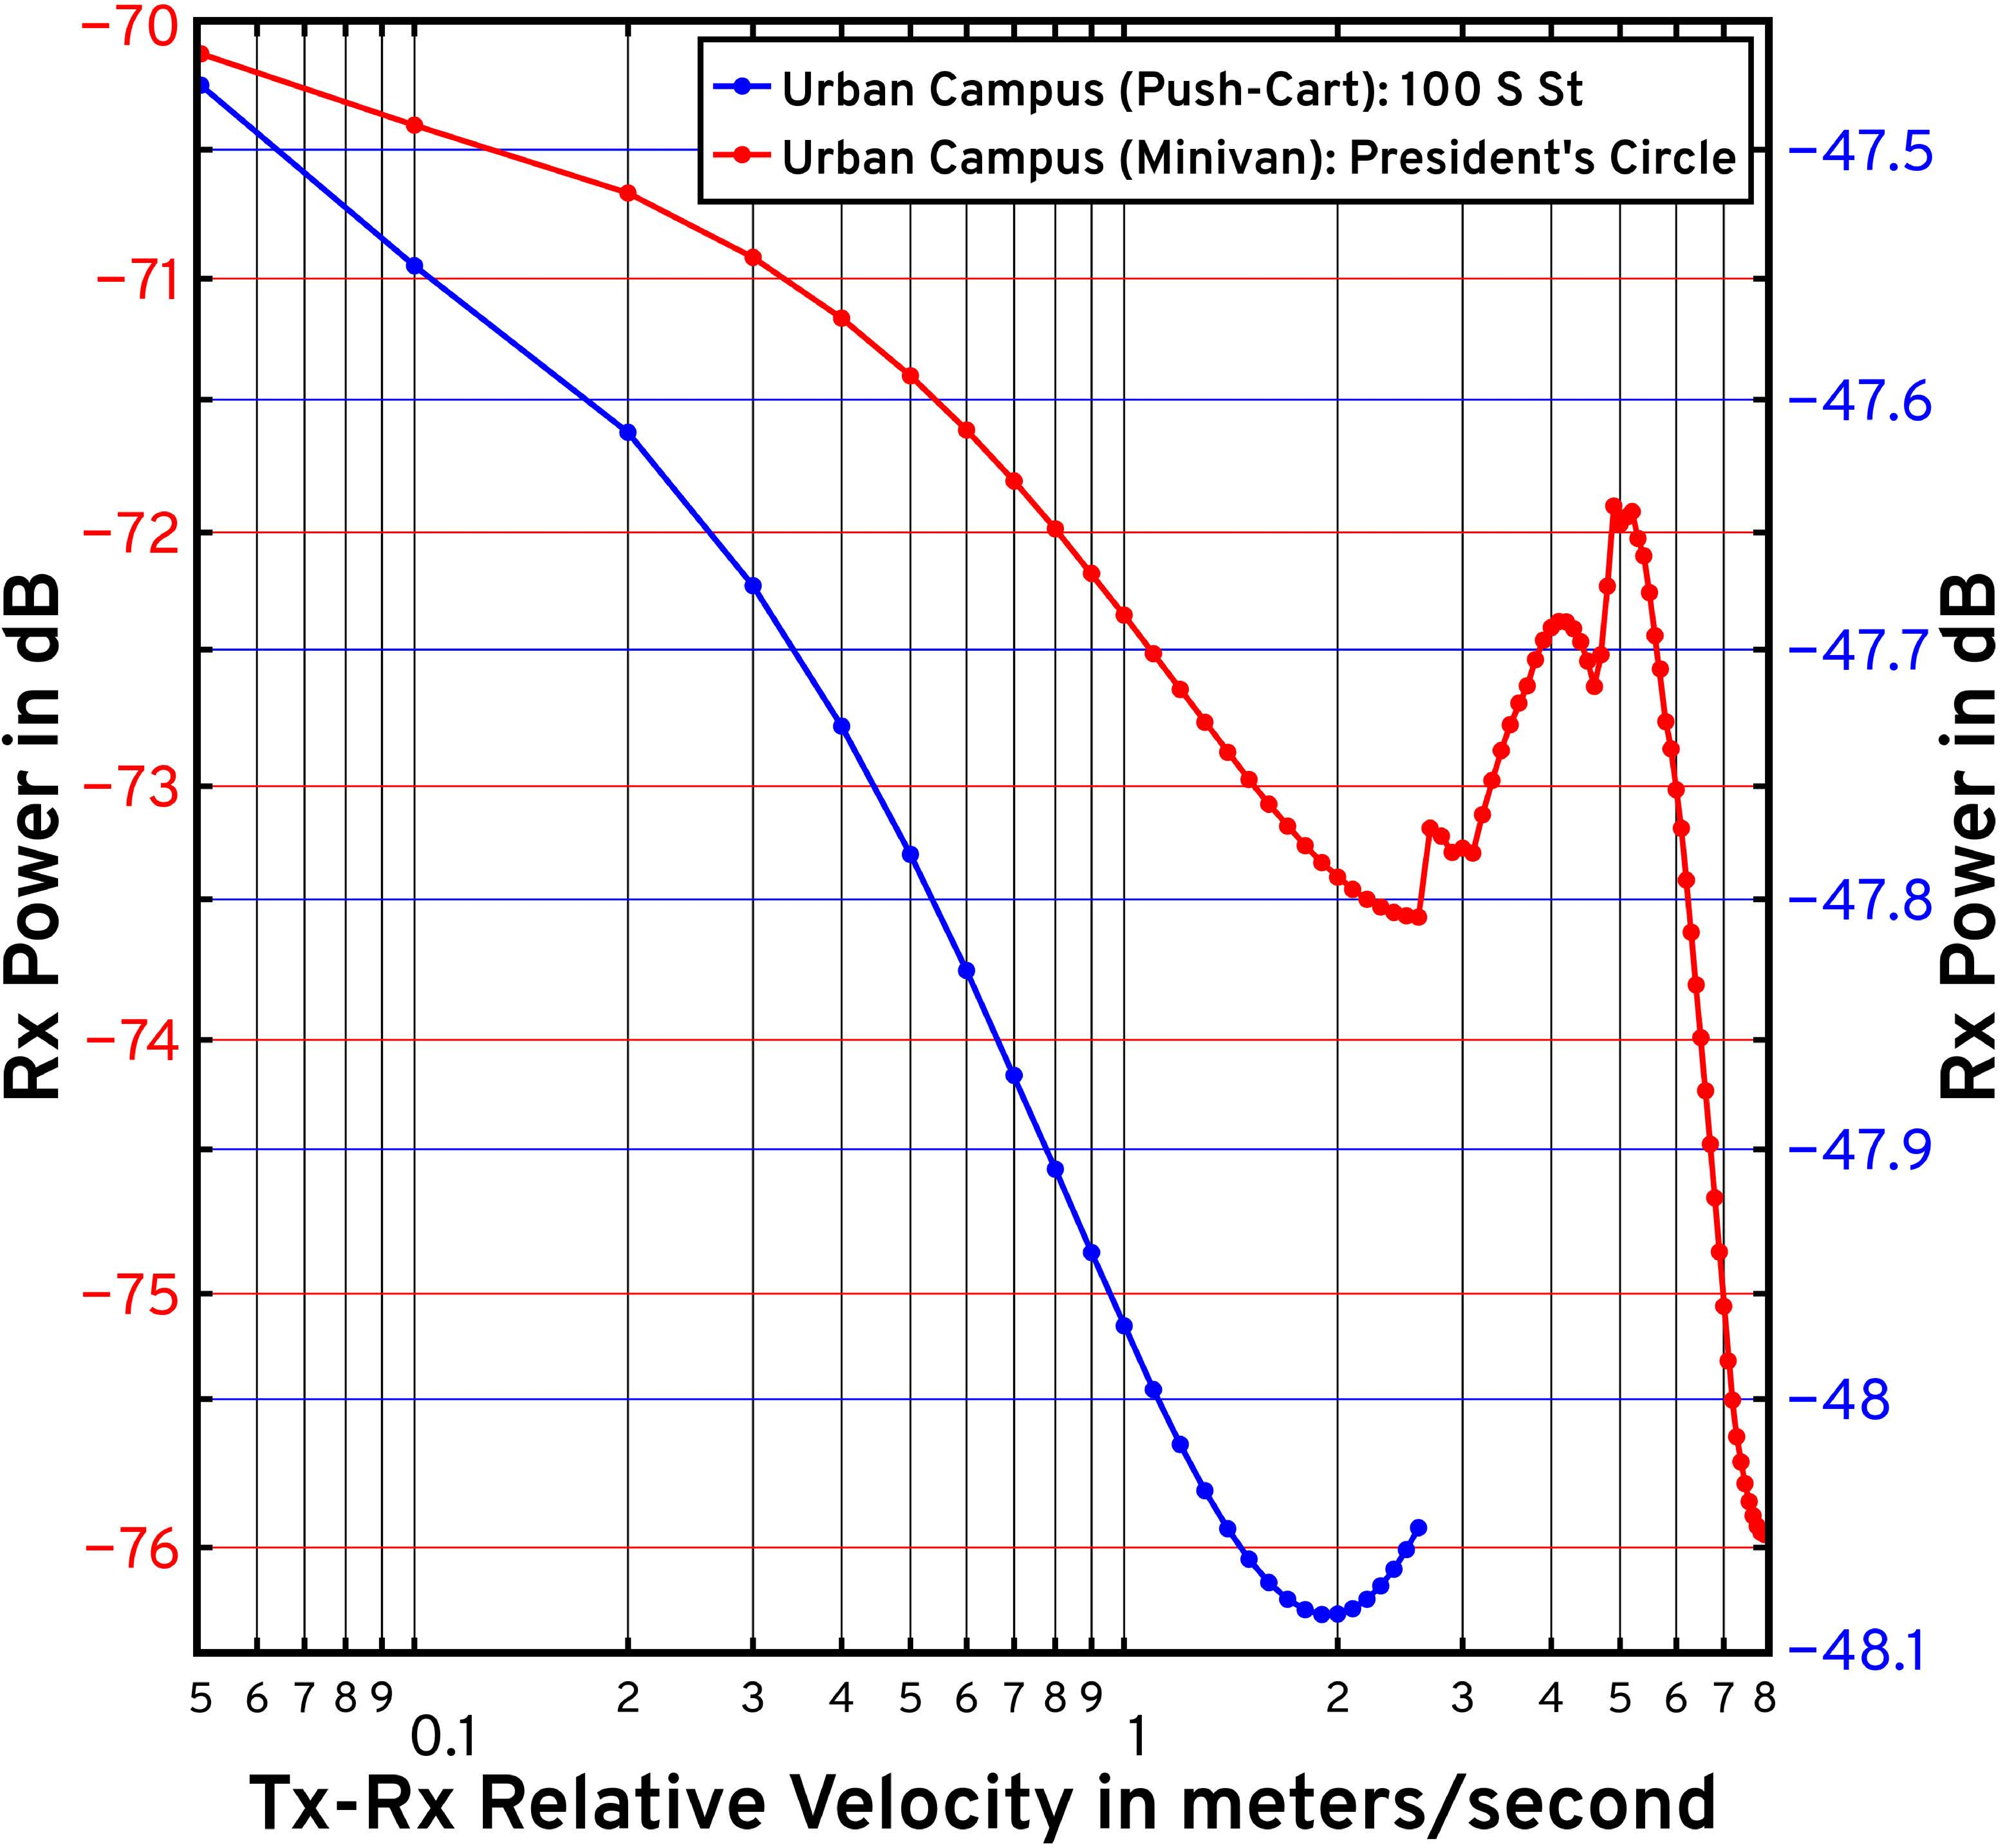
\includegraphics[width=1.0\linewidth]{figs/rx_power_vs_velocity.pdf}
        \caption{Received Signal Power vs Tx-Rx Relative Velocity}
        \label{F8b}
    \end{subfigure}
    \vspace{-8mm}
    \caption{A plot of the spatial autocorrelation coefficient under separations in alignment accuracy, i.e., $\rho(\Delta \phi)$ vs log alignment accuracy in degrees (a); and a plot of the received signal power (in dB) under variations in the Tx-Rx relative velocity (in meters/second) (b) for urban campus routes, i.e., President's Circle (Rx is on minivan) and $100$ S St (Rx is on a push-cart).}
    \label{F8}
\end{figure*}

For the MPC at delay bin $\tau_{l} \in \boldsymbol{\tau}$, the local amplitude mean (temporal average) across the set of measurements collected at a route configuration index $i \in \mathcal{I}$ is $A_{i}(\tau_{l}) \triangleq \frac{1}{J_{i}}\sum_{j = 1}^{J_{i}}\ A_{i,j}(\tau_{l})$. Let $\mathbf{d} \triangleq \{d_{1},d_{2},{\dots},d_{K}\}$ be the Tx-Rx distance bins (quantization of distances) along this route $\mathcal{R}$; similarly, let $\boldsymbol{\phi} \triangleq \{\phi_{1},\phi_{2},{\dots},\phi_{M}\}$ denote the Tx-Rx alignment accuracy bins. Then, we define $\mathcal{I}(d_{k}, \phi_{m}) \triangleq \{i \in \mathcal{I}: \norm{\mathbf{x}_{i} - \mathbf{y}_{i}} \approx d_{k}, \phi_{i} \approx \phi_{m}\}$ as the set of route configuration indices for which their Tx-Rx distance belongs to distance bin $d_{k}$ and their Tx-Rx alignment accuracy belongs to alignment bin $\phi_{m}$ (note that in this definition, the binning-based quantization is represented with the $\approx$ notation). Next, to study signal decoherence behavior under distance separations, for a route configuration index $i \in \mathcal{I}$ with its Tx-Rx distance in distance bin $d_{k} \in \mathbf{d}$ and Tx-Rx alignment accuracy in alignment bin $\phi_{m} \in \boldsymbol{\phi}$, we define the amplitude sample mean (spatial average) of the MPC at delay bin $\tau_{l} \in \boldsymbol{\tau}$ as $\mu_{i}(\tau_{l}) = \frac{1}{|\mathcal{I}(d_{k}, \phi_{m})|}\sum_{\iota = 1}^{|\mathcal{I}(d_{k}, \phi_{m})|}\ A_{\iota}(\tau_{l})$; similarly, for a route configuration index $i' \in \mathcal{I}$ with its Tx-Rx distance in distance bin $d_{k'} \in \mathbf{d}$ and Tx-Rx alignment accuracy in alignment bin $\phi_{m} \in \boldsymbol{\phi}$, we define the amplitude sample mean (spatial average) of the MPC at delay bin $\tau_{l} \in \boldsymbol{\tau}$ as $\mu_{i'}(\tau_{l}) = \frac{1}{|\mathcal{I}(d_{k'}, \phi_{m})|}\sum_{\iota = 1}^{|\mathcal{I}(d_{k'}, \phi_{m})|}\ A_{\iota}(\tau_{l})$. Note that the sets used to compute these amplitude sample means for $i, i' \in \mathcal{I}$ could potentially differ only in their Tx-Rx distance bin, i.e., consistent with the condition~\eqref{E}, they should belong to the same alignment accuracy bin. In a similar vein, consistent with the condition~\eqref{Ea}, for alignment accuracy separations, the amplitude sample means $\mu_{i}(\tau_{l})$ and $\mu_{i'}(\tau_{l})$ involve index sets that could potentially differ only in their Tx-Rx alignment accuracy bins, i.e., they should belong to the same distance bin. Thus, using these definitions of the amplitude sample means and with the index sets~\eqref{E} and~\eqref{Ea} serving as evaluation conditions, we define the spatial autocorrelation coefficient $\rho$ under a separation in distance $\Delta d$ and a separation in alignment accuracy $\Delta \phi$ as
\begin{align}\label{SC}
    &\rho(\Delta d) = \frac{\frac{1}{|\mathcal{I}(\Delta d)|}\sum_{(i,i') \in \mathcal{I}(\Delta d)}\Bigg[\sum_{l = 1}^{L}\bigg(\Big(A_{i}(\tau_{l}) - \mu_{i}(\tau_{l})\Big)\Big(A_{i'}(\tau_{l}) - \mu_{i'}(\tau_{l})\Big)\bigg)\Bigg]}{\frac{1}{|\mathcal{I}|}\sum_{i \in \mathcal{I}}\bigg[\sum_{l = 1}^{L}\Big(A_{i}(\tau_{l}) - \mu_{i}(\tau_{l})\Big)^{2}\bigg]},\\
    &\rho(\Delta \phi) = \frac{\frac{1}{|\mathcal{I}(\Delta \phi)|}\sum_{(i,i') \in \mathcal{I}(\Delta \phi)}\Bigg[\sum_{l = 1}^{L}\bigg(\Big(A_{i}(\tau_{l}) - \mu_{i}(\tau_{l})\Big)\Big(A_{i'}(\tau_{l}) - \mu_{i'}(\tau_{l})\Big)\bigg)\Bigg]}{\frac{1}{|\mathcal{I}|}\sum_{i \in \mathcal{I}}\bigg[\sum_{l = 1}^{L}\Big(A_{i}(\tau_{l}) - \mu_{i}(\tau_{l})\Big)^{2}\bigg]}.
\end{align}

As a result of the framework described above, Fig.~\ref{F7b} illustrates the spatial consistency curves as a function of the separations in distance for the urban campus, suburban neighborhood, and foliage environment routes. We note decreasing correlation trends between the recorded power delay profile samples under increasing distance separation. Similarly, Fig.~\ref{F8a} depicts the variation of the spatial autocorrelation coefficient under increasing levels of misalignment between the Tx and Rx antennas while traversing the urban campus, suburban neighborhood, and foliage environment routes. We observe rapid decorrelation across the evaluated samples even at small amounts of misalignment, highlighting the highly-directional characteristics of our WR-$28$ horn antennas, and illustrating the need for accurate beam-steering in mmWave V$2$X networks. Note that, in Fig.~\ref{F7b} and Fig.~\ref{F8a}, the channel does not get fully decorrelated since in our beam-steered setup, the line-of-sight component always remains significant. Lastly, Fig.~\ref{F8b} depicts the received signal power at the Rx under variations in the Tx-Rx relative velocity around the urban campus routes onsite wherein the Rx is mounted either on a push-cart ($100$ S St, \SI{0}{mph} to \SI{5}{mph}) or on a minivan (President's Circle, \SI{0}{mph} to \SI{18}{mph}). Here, we observe considerable drops in received power under minor velocity variations due to response latencies and misalignments introduced into our mechanical beam-steering platform when the Rx is driven away from the Tx, reiterating the need for an accurate and responsive beam-steering design in mmWave V$2$X applications.
\begin{figure*} [t]
    \centering
    \begin{subfigure}{0.4965\linewidth}
        \centering
        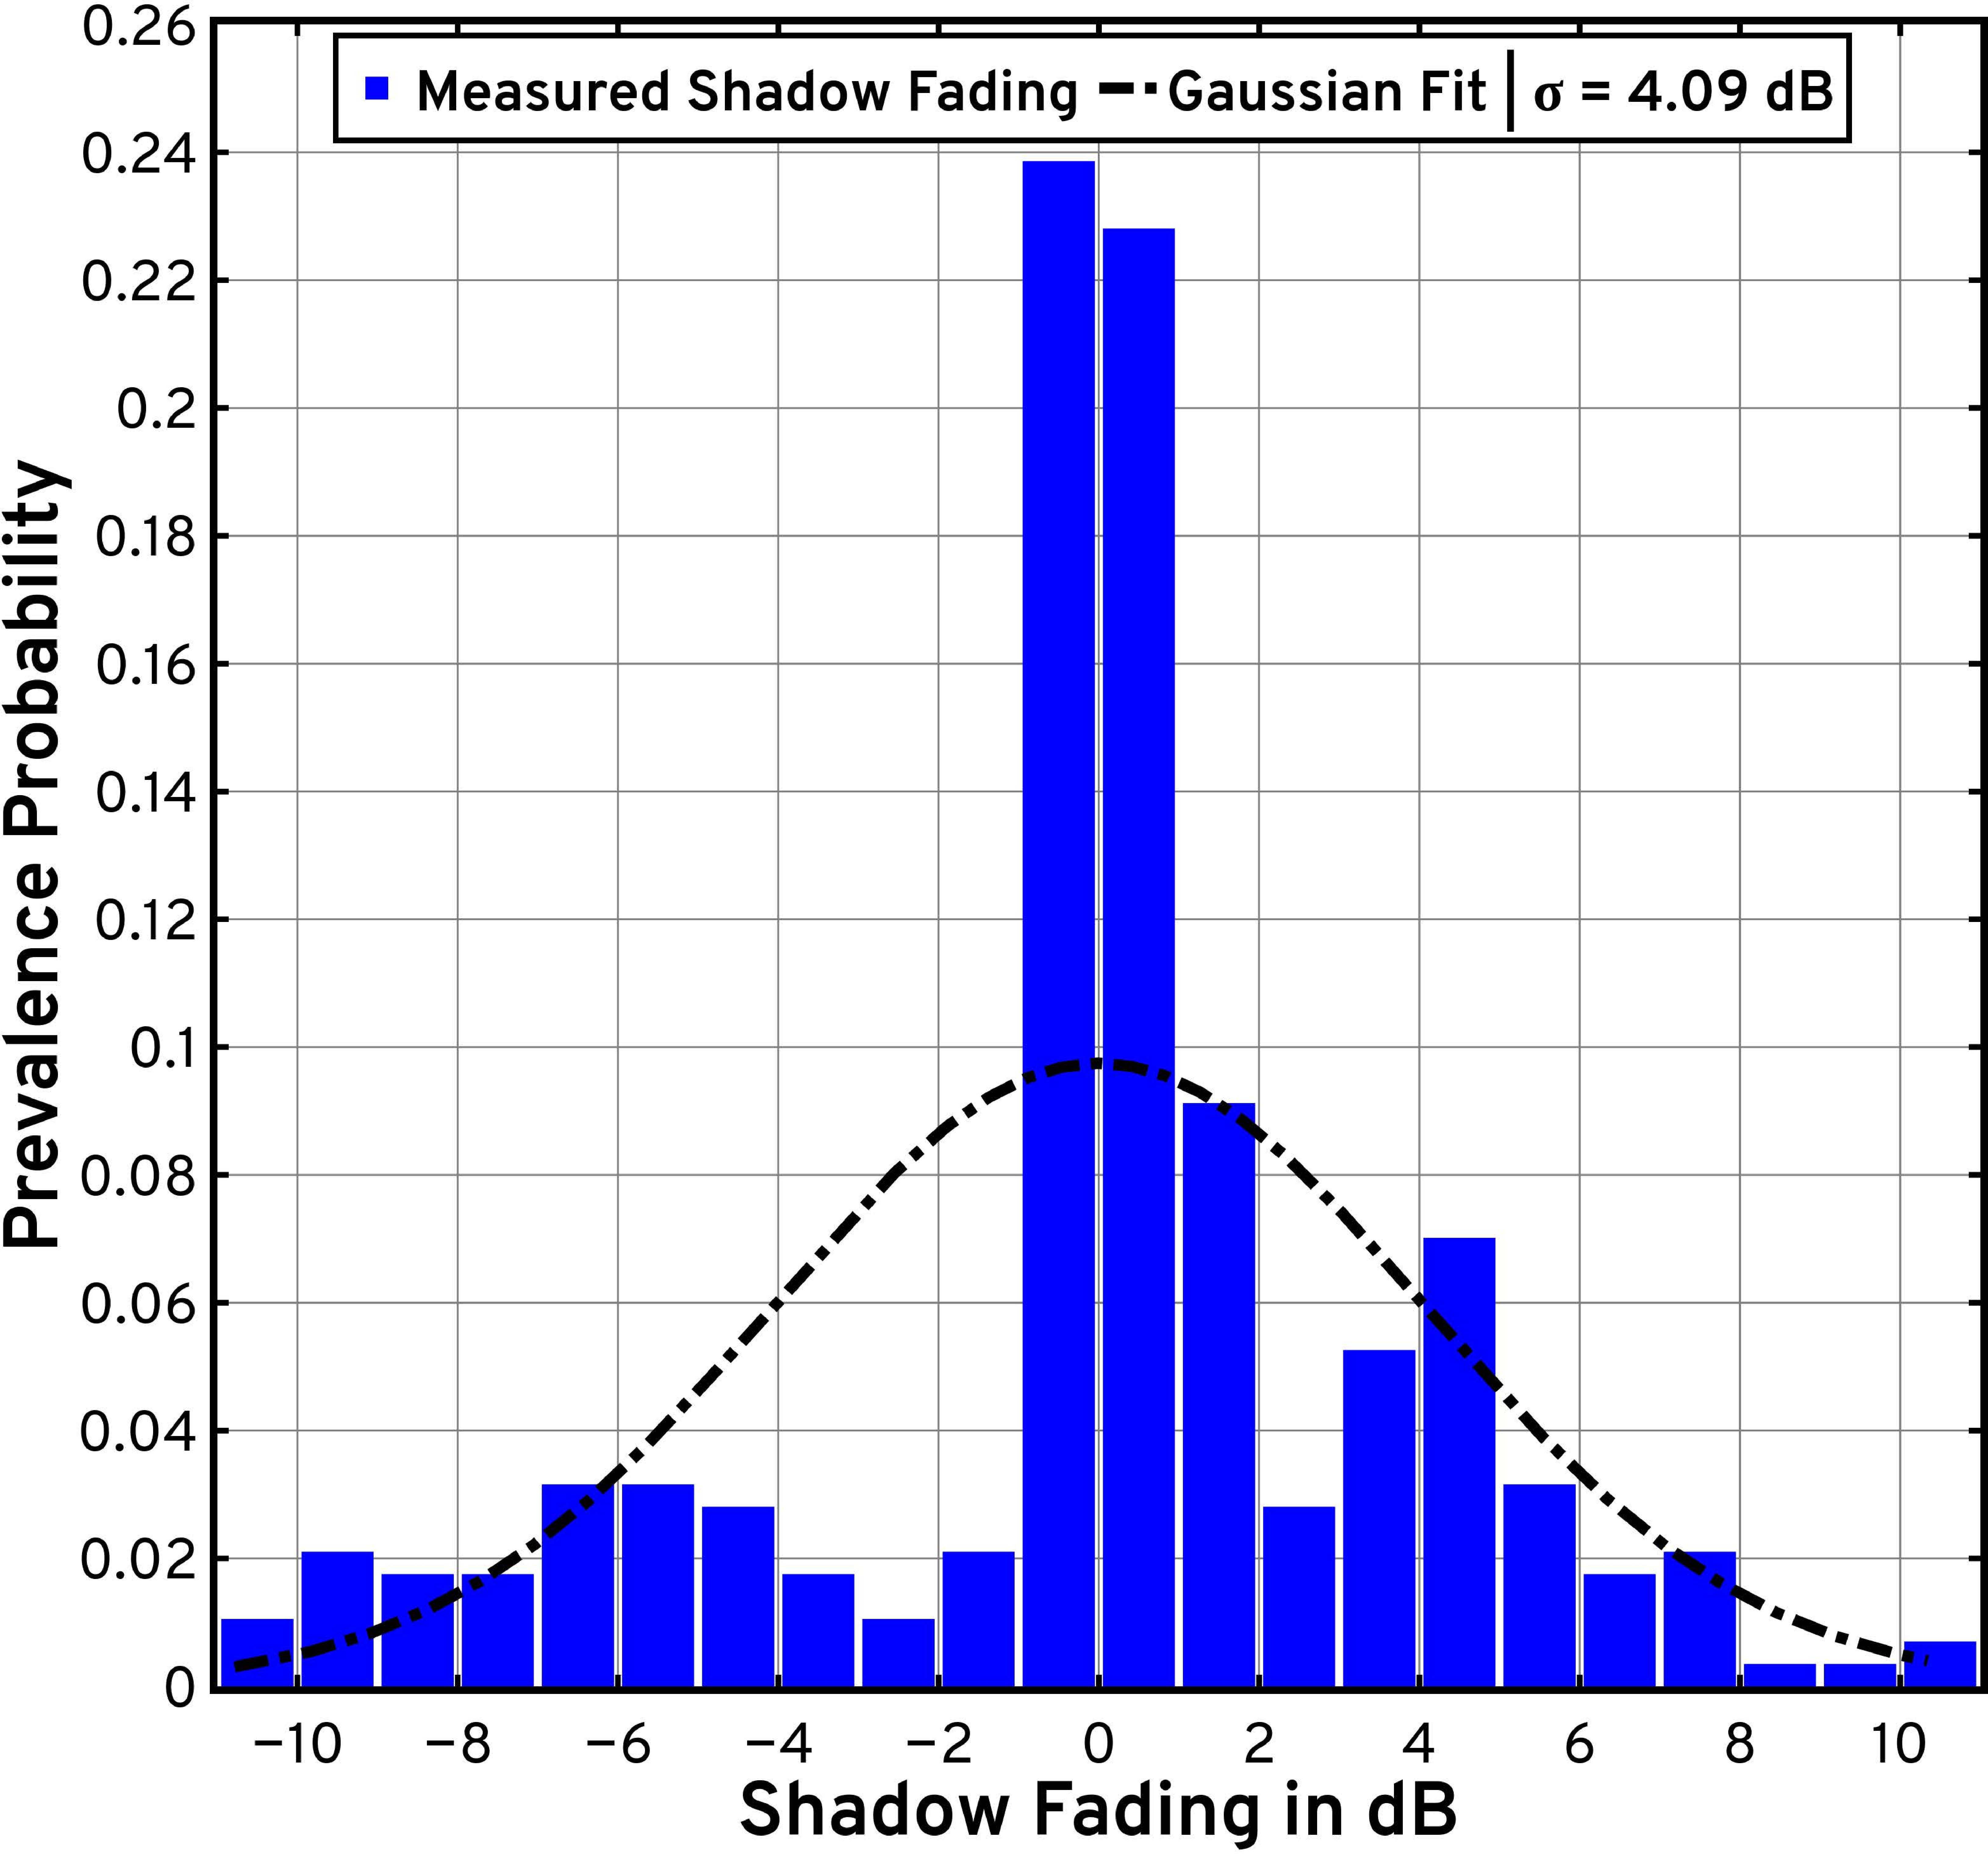
\includegraphics[width=1.0\linewidth]{figs/urban_campus_shadow_fading_1.pdf}
        \caption{Urban Campus (President's Circle)}
        \label{F9a}
    \end{subfigure}
    \begin{subfigure}{0.4935\linewidth}
        \centering
        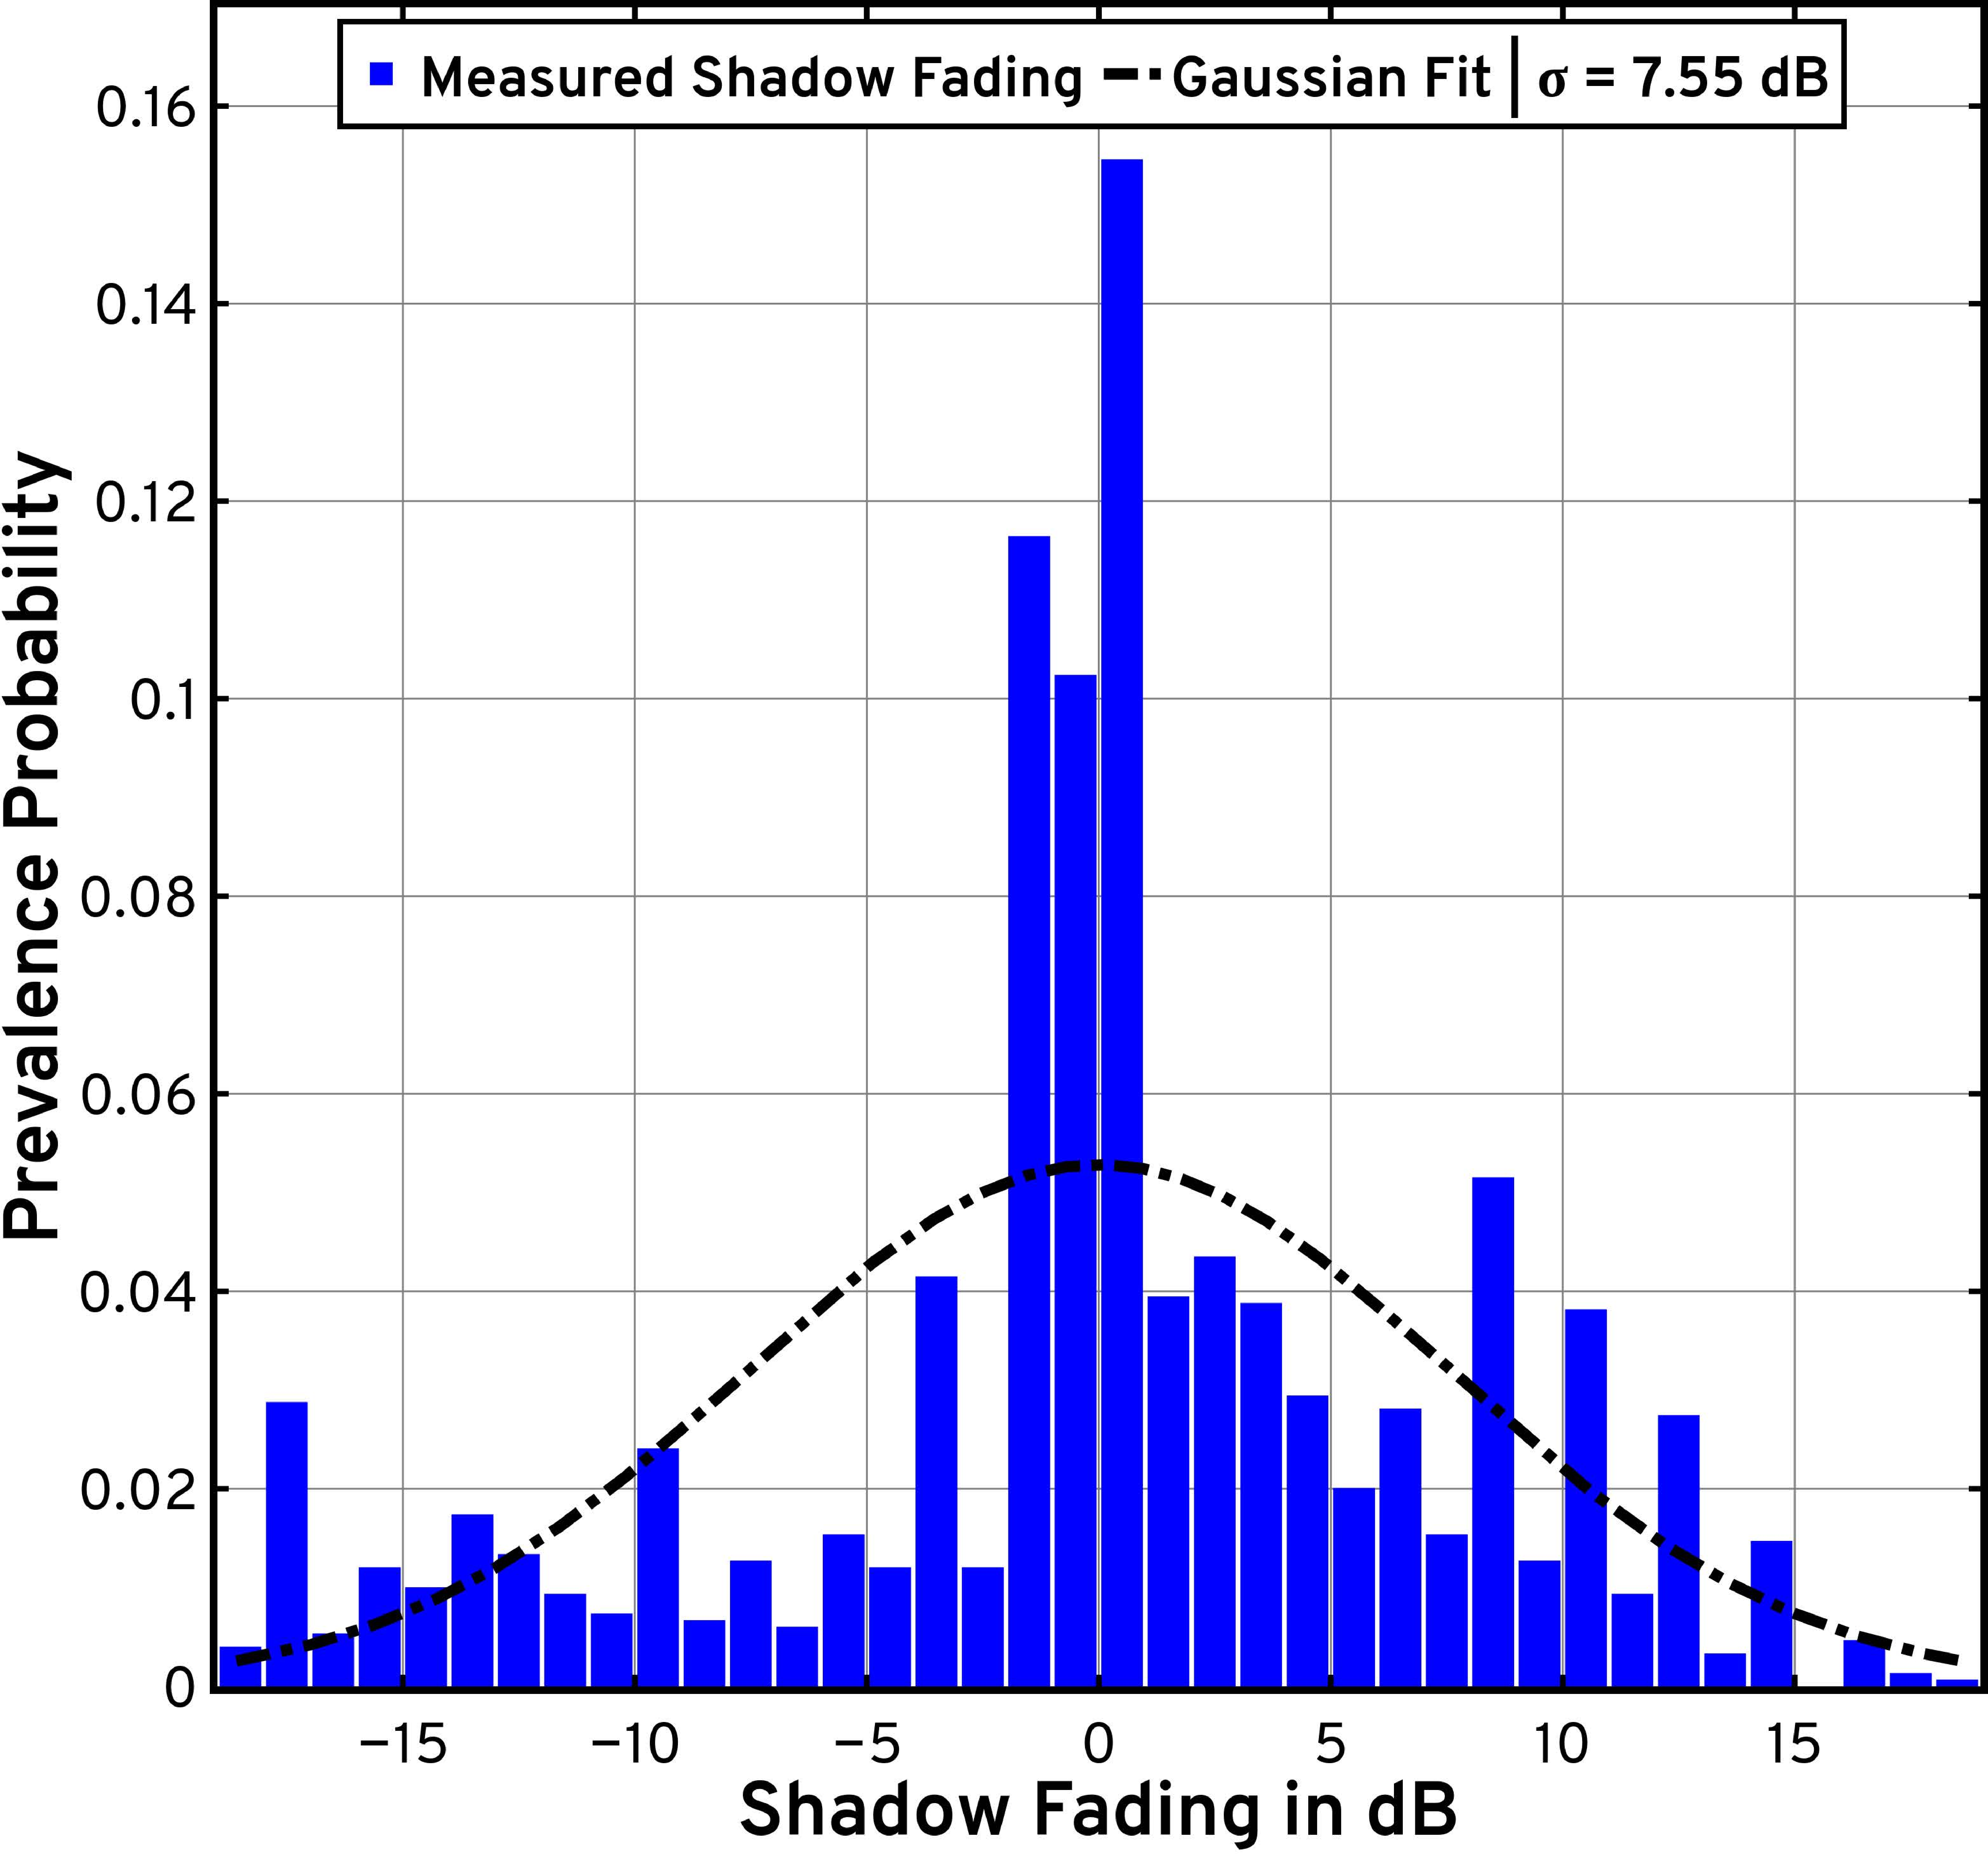
\includegraphics[width=1.0\linewidth]{figs/urban_campus_shadow_fading_2.pdf}
        \caption{Urban Campus ($100$ S St)}
        \label{F9b}
    \end{subfigure}
    \vspace{-8mm}
    \caption{The histograms and their corresponding Gaussian fits for the shadow fading (in dB) experienced by mmWave signals along the urban campus routes onsite, i.e., President's Circle (a) (Rx is on a minivan) and $100$ S St (b) (Rx is on a push-cart).}
    \label{F9}
\end{figure*}

\noindent{\textbf{Shadowing \& Dynamic Blockages}}: The shadow fading plots for the two urban campus routes, i.e., President's Circle (Rx on a minivan) and $100$ S St (Rx on a push-cart), are depicted in Fig.~\ref{F9a} and Fig.~\ref{F9b}. Averaging out the effects of multipath fading across several measurements over a \SI{1}{\meter} distance resolution~\cite{Averaging_Threshold}, these plots depict the histograms of the deviations of the measured pathloss values from those provided by the linear models fitted to our measurements in Fig.~\ref{F7a}; upon visualizing these histograms for the two urban campus routes (dominated by tall buildings), we fit Gaussian curves (standard normals) to obtain the log-normal shadow fading distributions typically seen in the state-of-the-art~\cite{DopplerHST}. Herein, as is evident from the structural profiles of the two routes (see Fig.~\ref{F5a} and Fig.~\ref{F5b}), we observe that the urban campus route around $100$ S St exhibits a larger shadowing impact ($\sigma{=}$\SI{7.55}{\deci\bel}) relative to that around President's Circle ($\sigma{=}$\SI{4.09}{\deci\bel}) due to the higher obstacle density (geometry-induced losses) around $100$ S St.
\begin{figure*} [t]
    \centering
    \begin{subfigure}{0.5\linewidth}
        \centering
        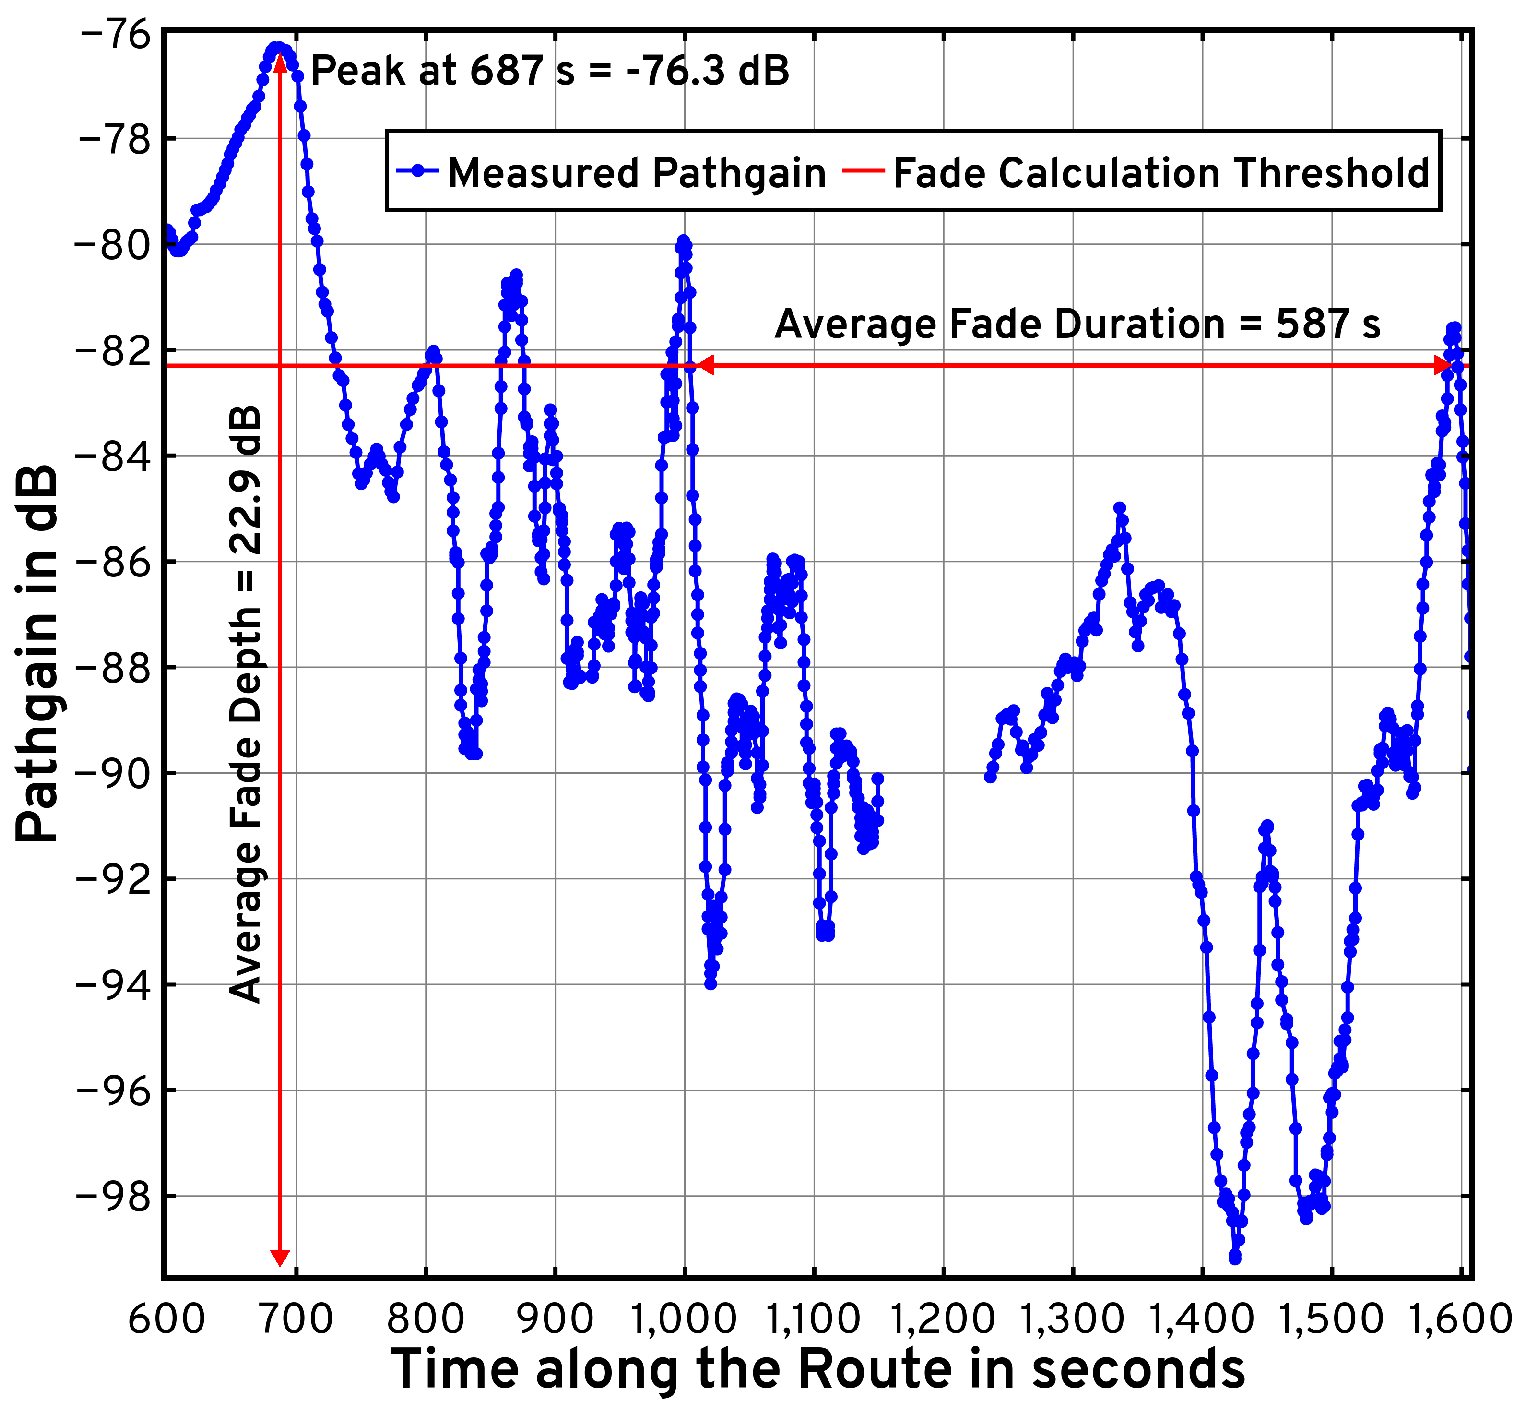
\includegraphics[width=1.0\linewidth]{figs/urban_campus_pathgain_vs_time_gap_annotated.pdf}
        \caption{Urban Campus ($100$ S St)}
        \label{F10a}
    \end{subfigure}
    \begin{subfigure}{0.49\linewidth}
        \centering
        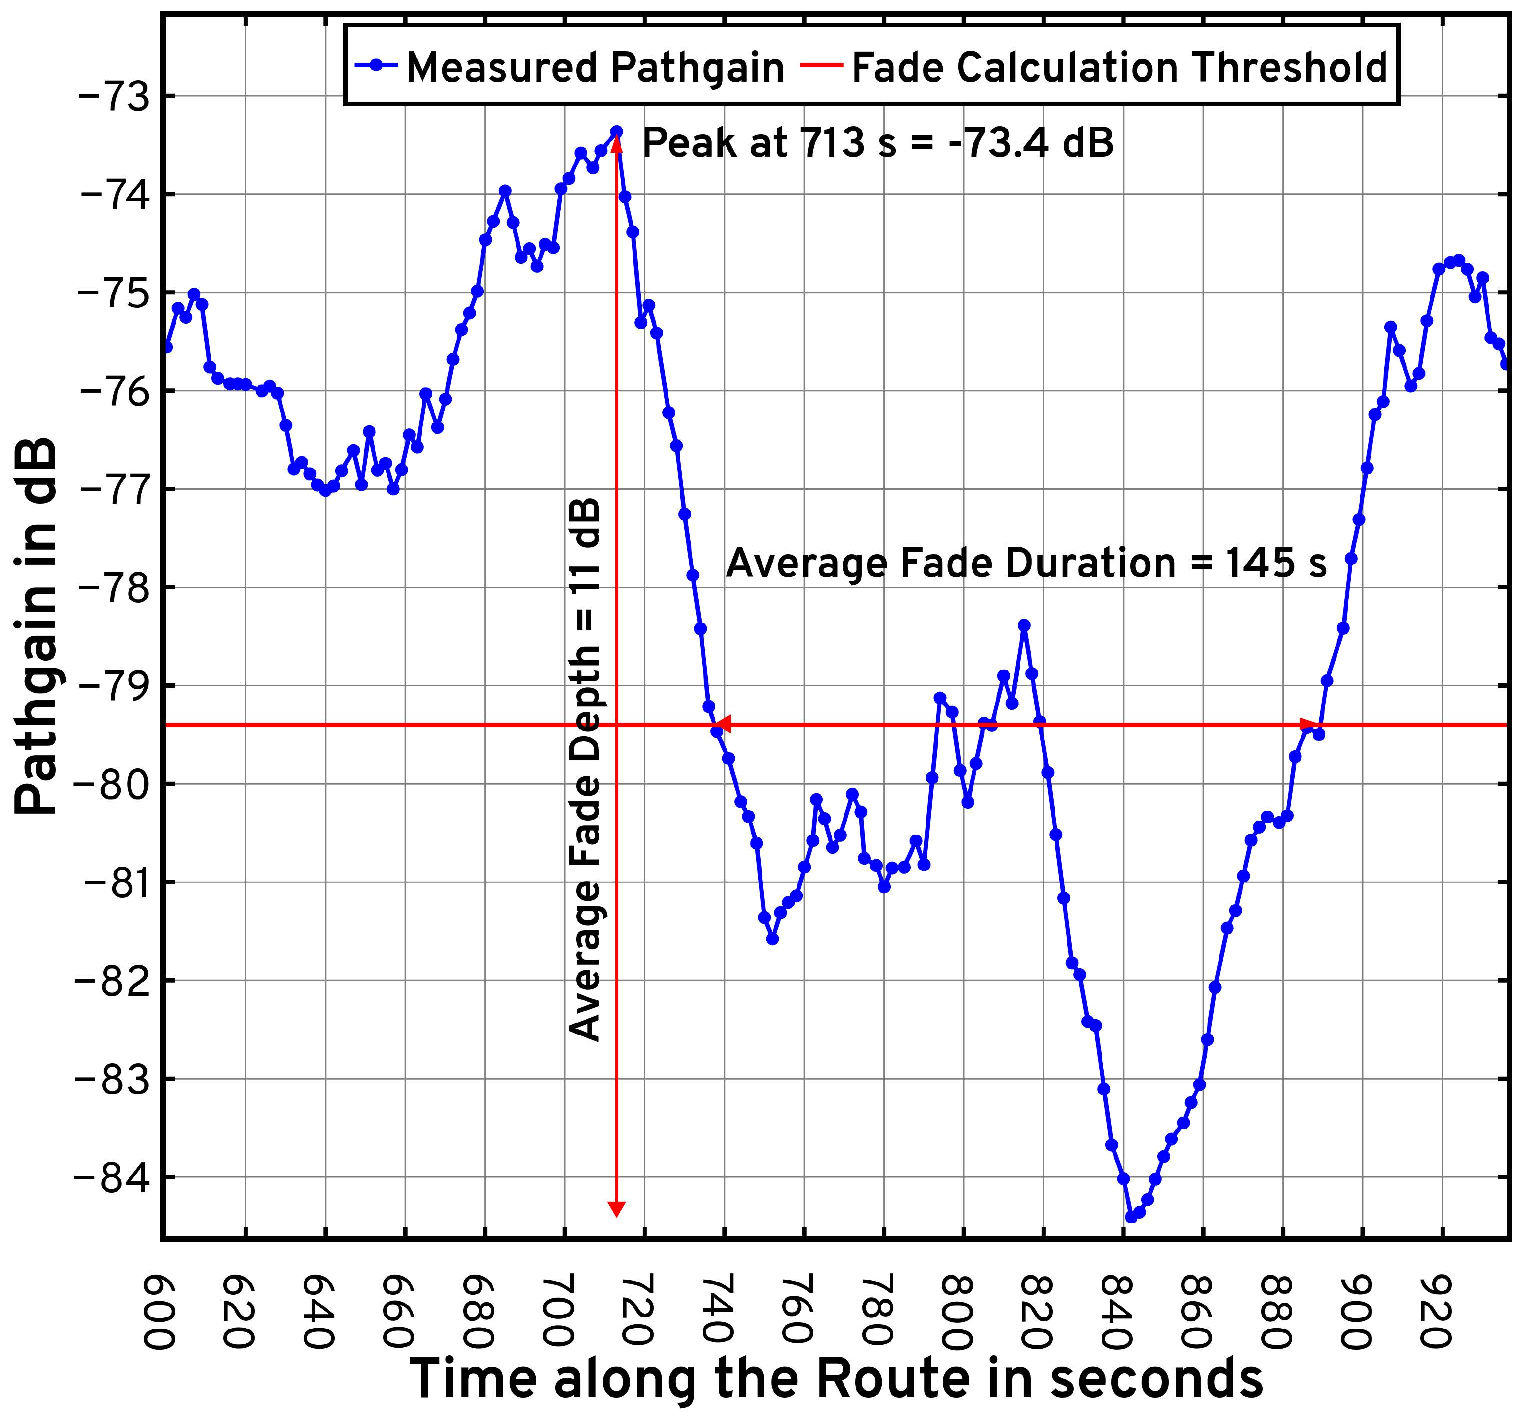
\includegraphics[width=1.0\linewidth]{figs/suburban_pathgain_vs_time_annotated.pdf}
        \caption{Suburban Neighborhood (S Wolcott St)}
        \label{F10b}
    \end{subfigure}
    \vspace{-8mm}
    \caption{The plots illustrating the small-scale fading (pathgain in dB vs time in seconds) experienced by mmWave signals along routes dominated by dynamic blockages (pedestrians and moving/parked vehicles), i.e., the urban campus route around $100$ S St (a) (Rx is on a push-cart) and the suburban neighborhood route around S Wolcott St (b) (Rx is again on a push-cart).}
    \label{F10}
\end{figure*}

Furthermore, the small-scale fading studies of \SI{28}{\giga\hertz} signals in V$2$X scenarios vis-à-vis the average fade depth and average fade duration metrics, along routes dominated by dynamic blockages (pedestrians and moving/parked vehicles), are illustrated in Fig.~\ref{F10a} and Fig.~\ref{F10b}. The pathgain versus route time plots depicted in these figures enable us to gather insights about the attenuations introduced into the signal path due to obstacles---specifically, obstacles that move in and move out of the signal path quickly. In V$2$X settings, these dynamic blockages typically include pedestrians and moving/parked vehicles, which cause additional attenuation (captured by the average fade depth metric) for the period over which they enter in and enter out of the signal's path (captured by the average fade duration metric). Studying these metrics in Fig.~\ref{F10a} and Fig.~\ref{F10b}, we note that the urban campus route around $100$ S St (Rx on a push-cart) exhibits a larger signal fade (${\approx}$\SI{23}{\deci\bel}) over a longer duration relative to the suburban neighborhood route (Rx on a push-cart, a signal fade of \SI{11}{\deci\bel}). This is due to the following two reasons: a) a higher vehicular density (moving/parked vehicles) around the $100$ S St route not only causes a larger signal fade for a longer duration, but also results in frequent drops in received signal strength as these obstacles move in and out of the signal path; and b) since the suburban neighborhood route had relatively negligible vehicular density and instead involved low frequency pedestrian traffic, mmWave signals around this neighborhood (S Wolcott St) experience smaller and infrequent fades over shorter durations. Additionally, evaluating these average fade depth and duration metrics against those reported by the D$2$D mmWave channel model~\cite{D2DHumanBlockage}, we note that, while the D$2$D model does not provide these fade metrics for vehicular traffic, the average fade depth reported by it for pedestrian traffic is between \SI{20}{}-\SI{25}{\deci\bel}, which is considerably higher than that observed in Fig.~\ref{F10b} (\SI{11}{\deci\bel} around S Wolcott St). In the next section, employing the MPCs and their associated parameters extracted via the SAGE algorithm detailed earlier, we describe our multipath clustering evaluations which includes cluster arrival and decay characteristics, RMS delay- and direction-spreads, and empirical validations of statistical mmWave channel models.
\vspace{-3mm}

% Numerical evaluations II: Multipath clustering and Channel model validations
\section{Multipath Clustering and Channel Modeling}\label{S5}
In this section, using the MPCs extracted via the SAGE algorithm~\cite{SAGE}, we outline multipath clustering studies involving cluster inter-arrival times, cluster decay attributes, and RMS delay- and direction-spreads. Also, to evaluate our measurements against the state-of-the-art, we employ the Kolmogorov-Smirnov statistic to facilitate experimental validations of widely-used mmWave channel models (SV~\cite{Indoor60G}, QD~\cite{QDC_NIST}, and stochastic~\cite{Indoor60G}) by providing a measure of the \emph{goodness of fit} between the empirical CDFs and those obtained from these statistical channel models.
\begin{figure*} [t]
    \centering
    \begin{subfigure}{0.495\linewidth}
        \centering
        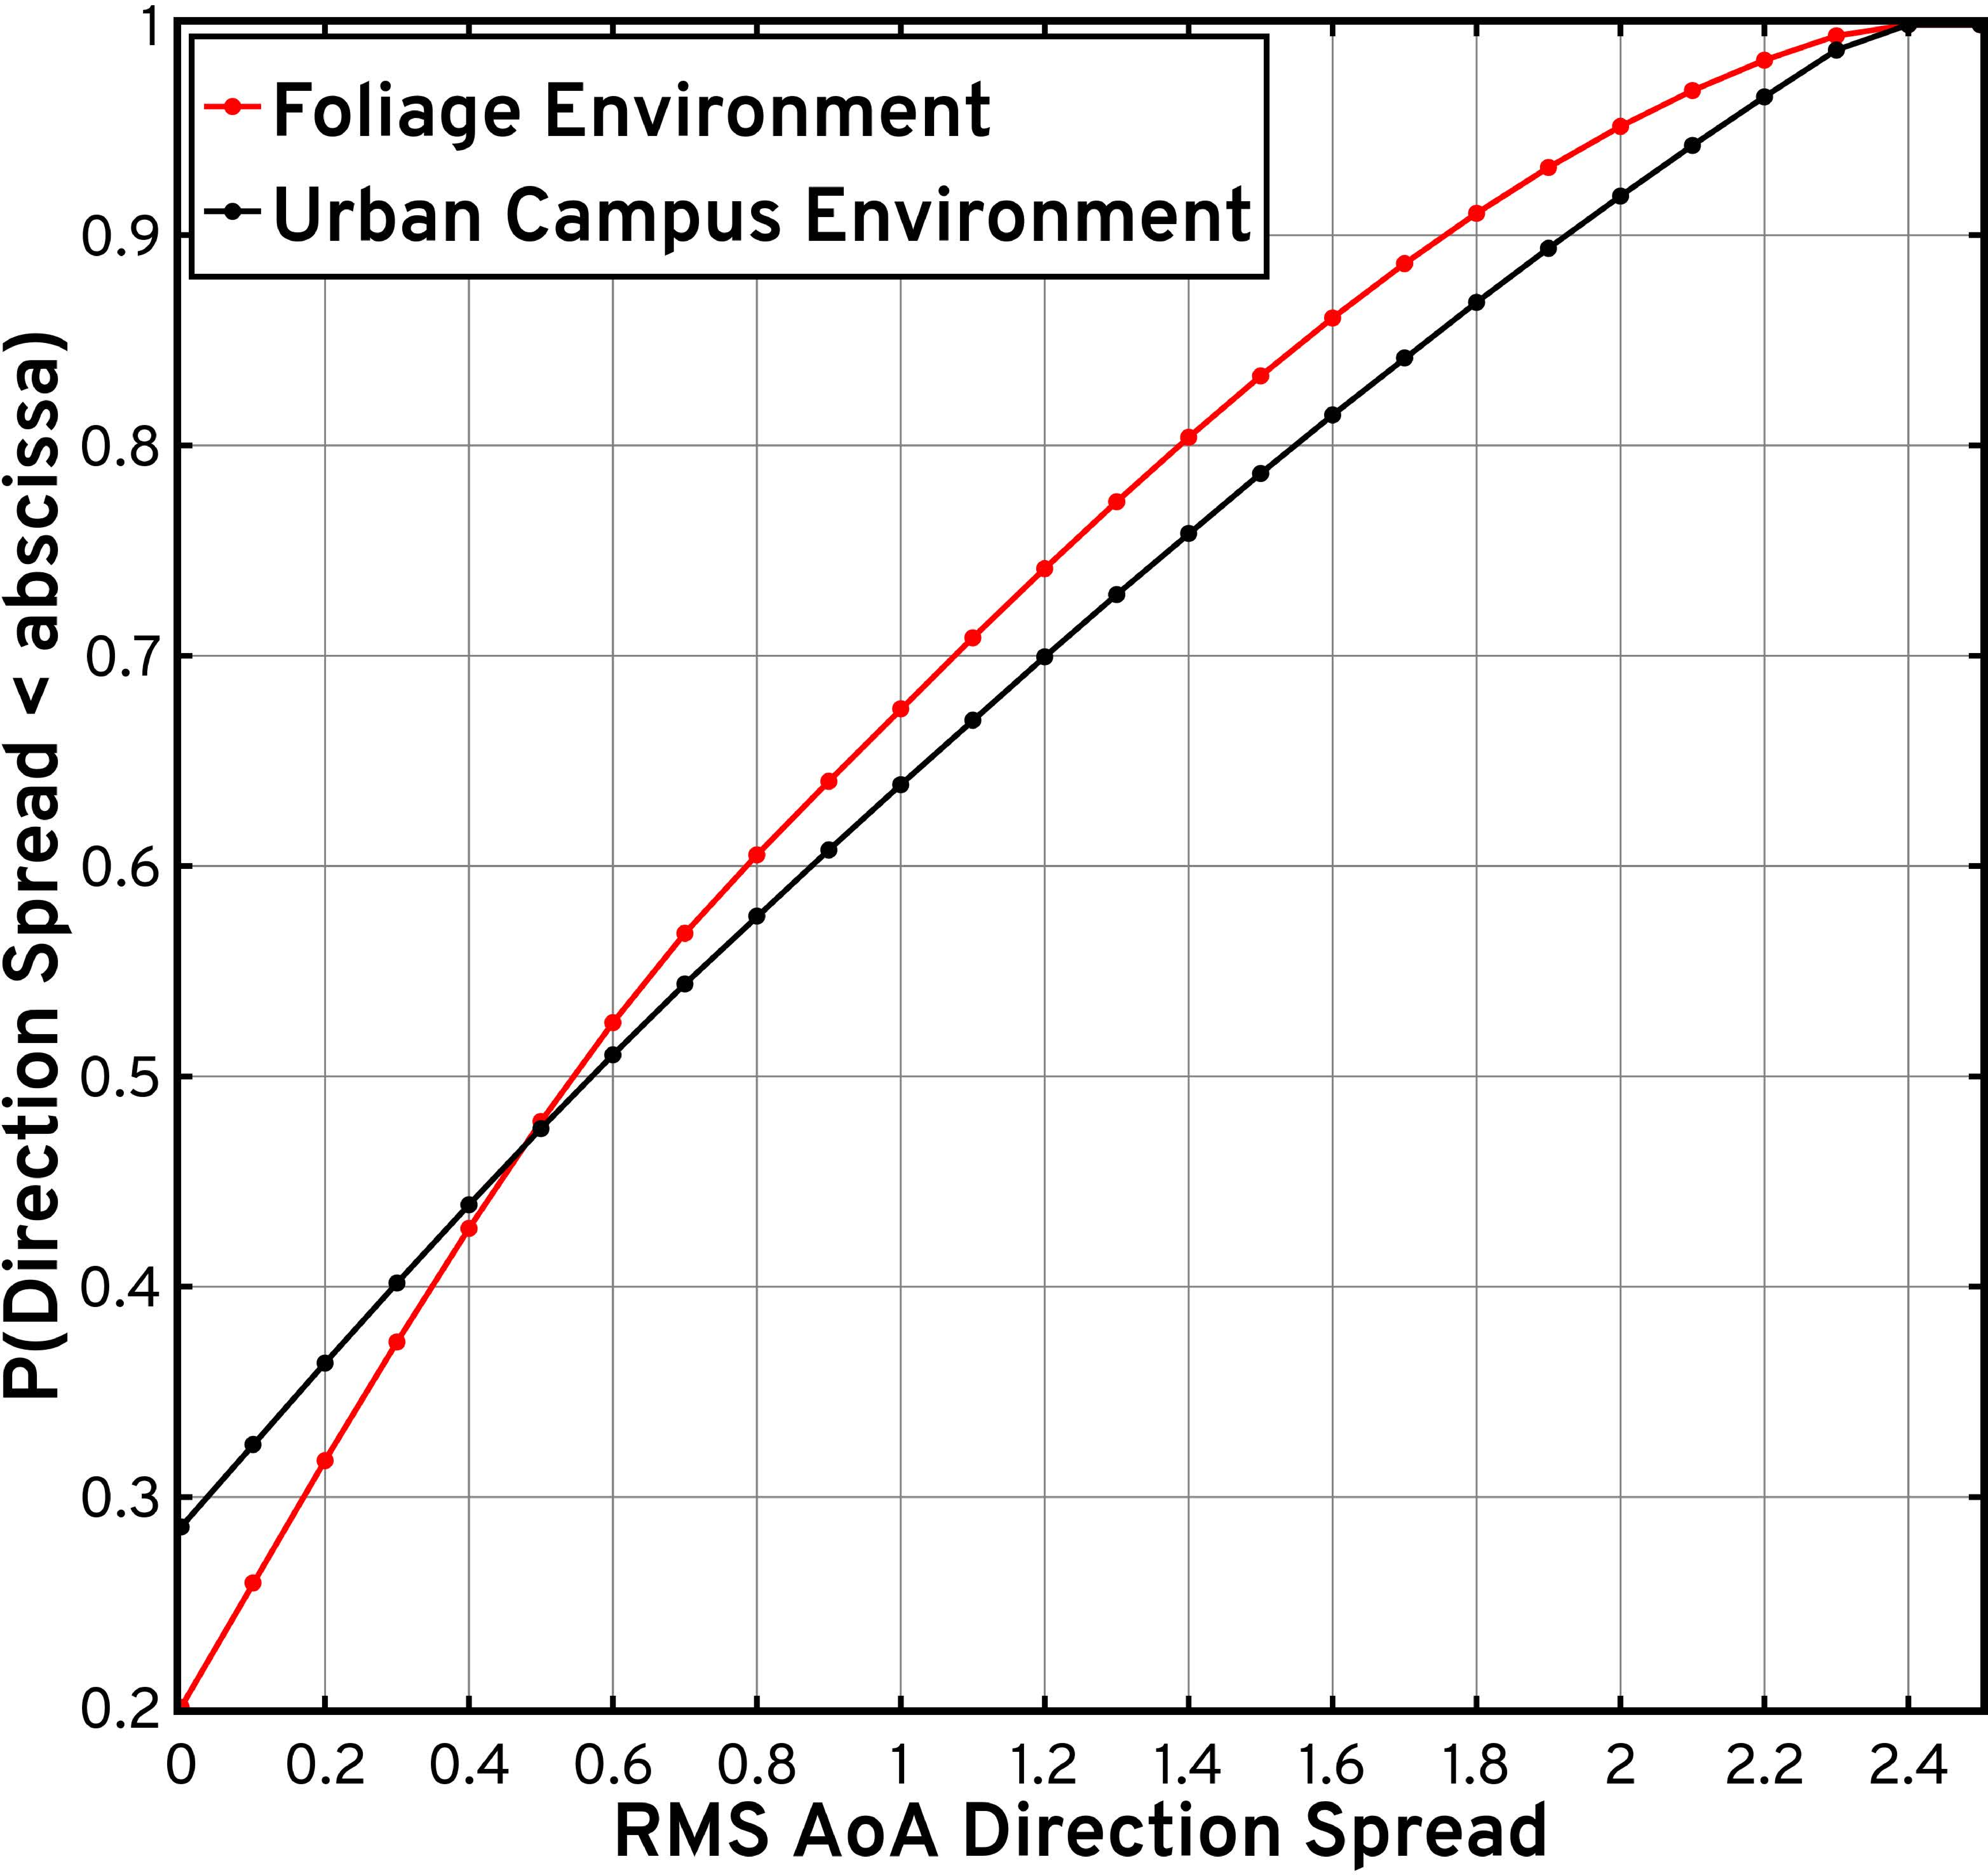
\includegraphics[width=1.0\linewidth]{figs/rms_direction_spread.pdf}
        \caption{RMS Delay-Spread CDFs}
        \label{F11a}
    \end{subfigure}
    \begin{subfigure}{0.495\linewidth}
        \centering
        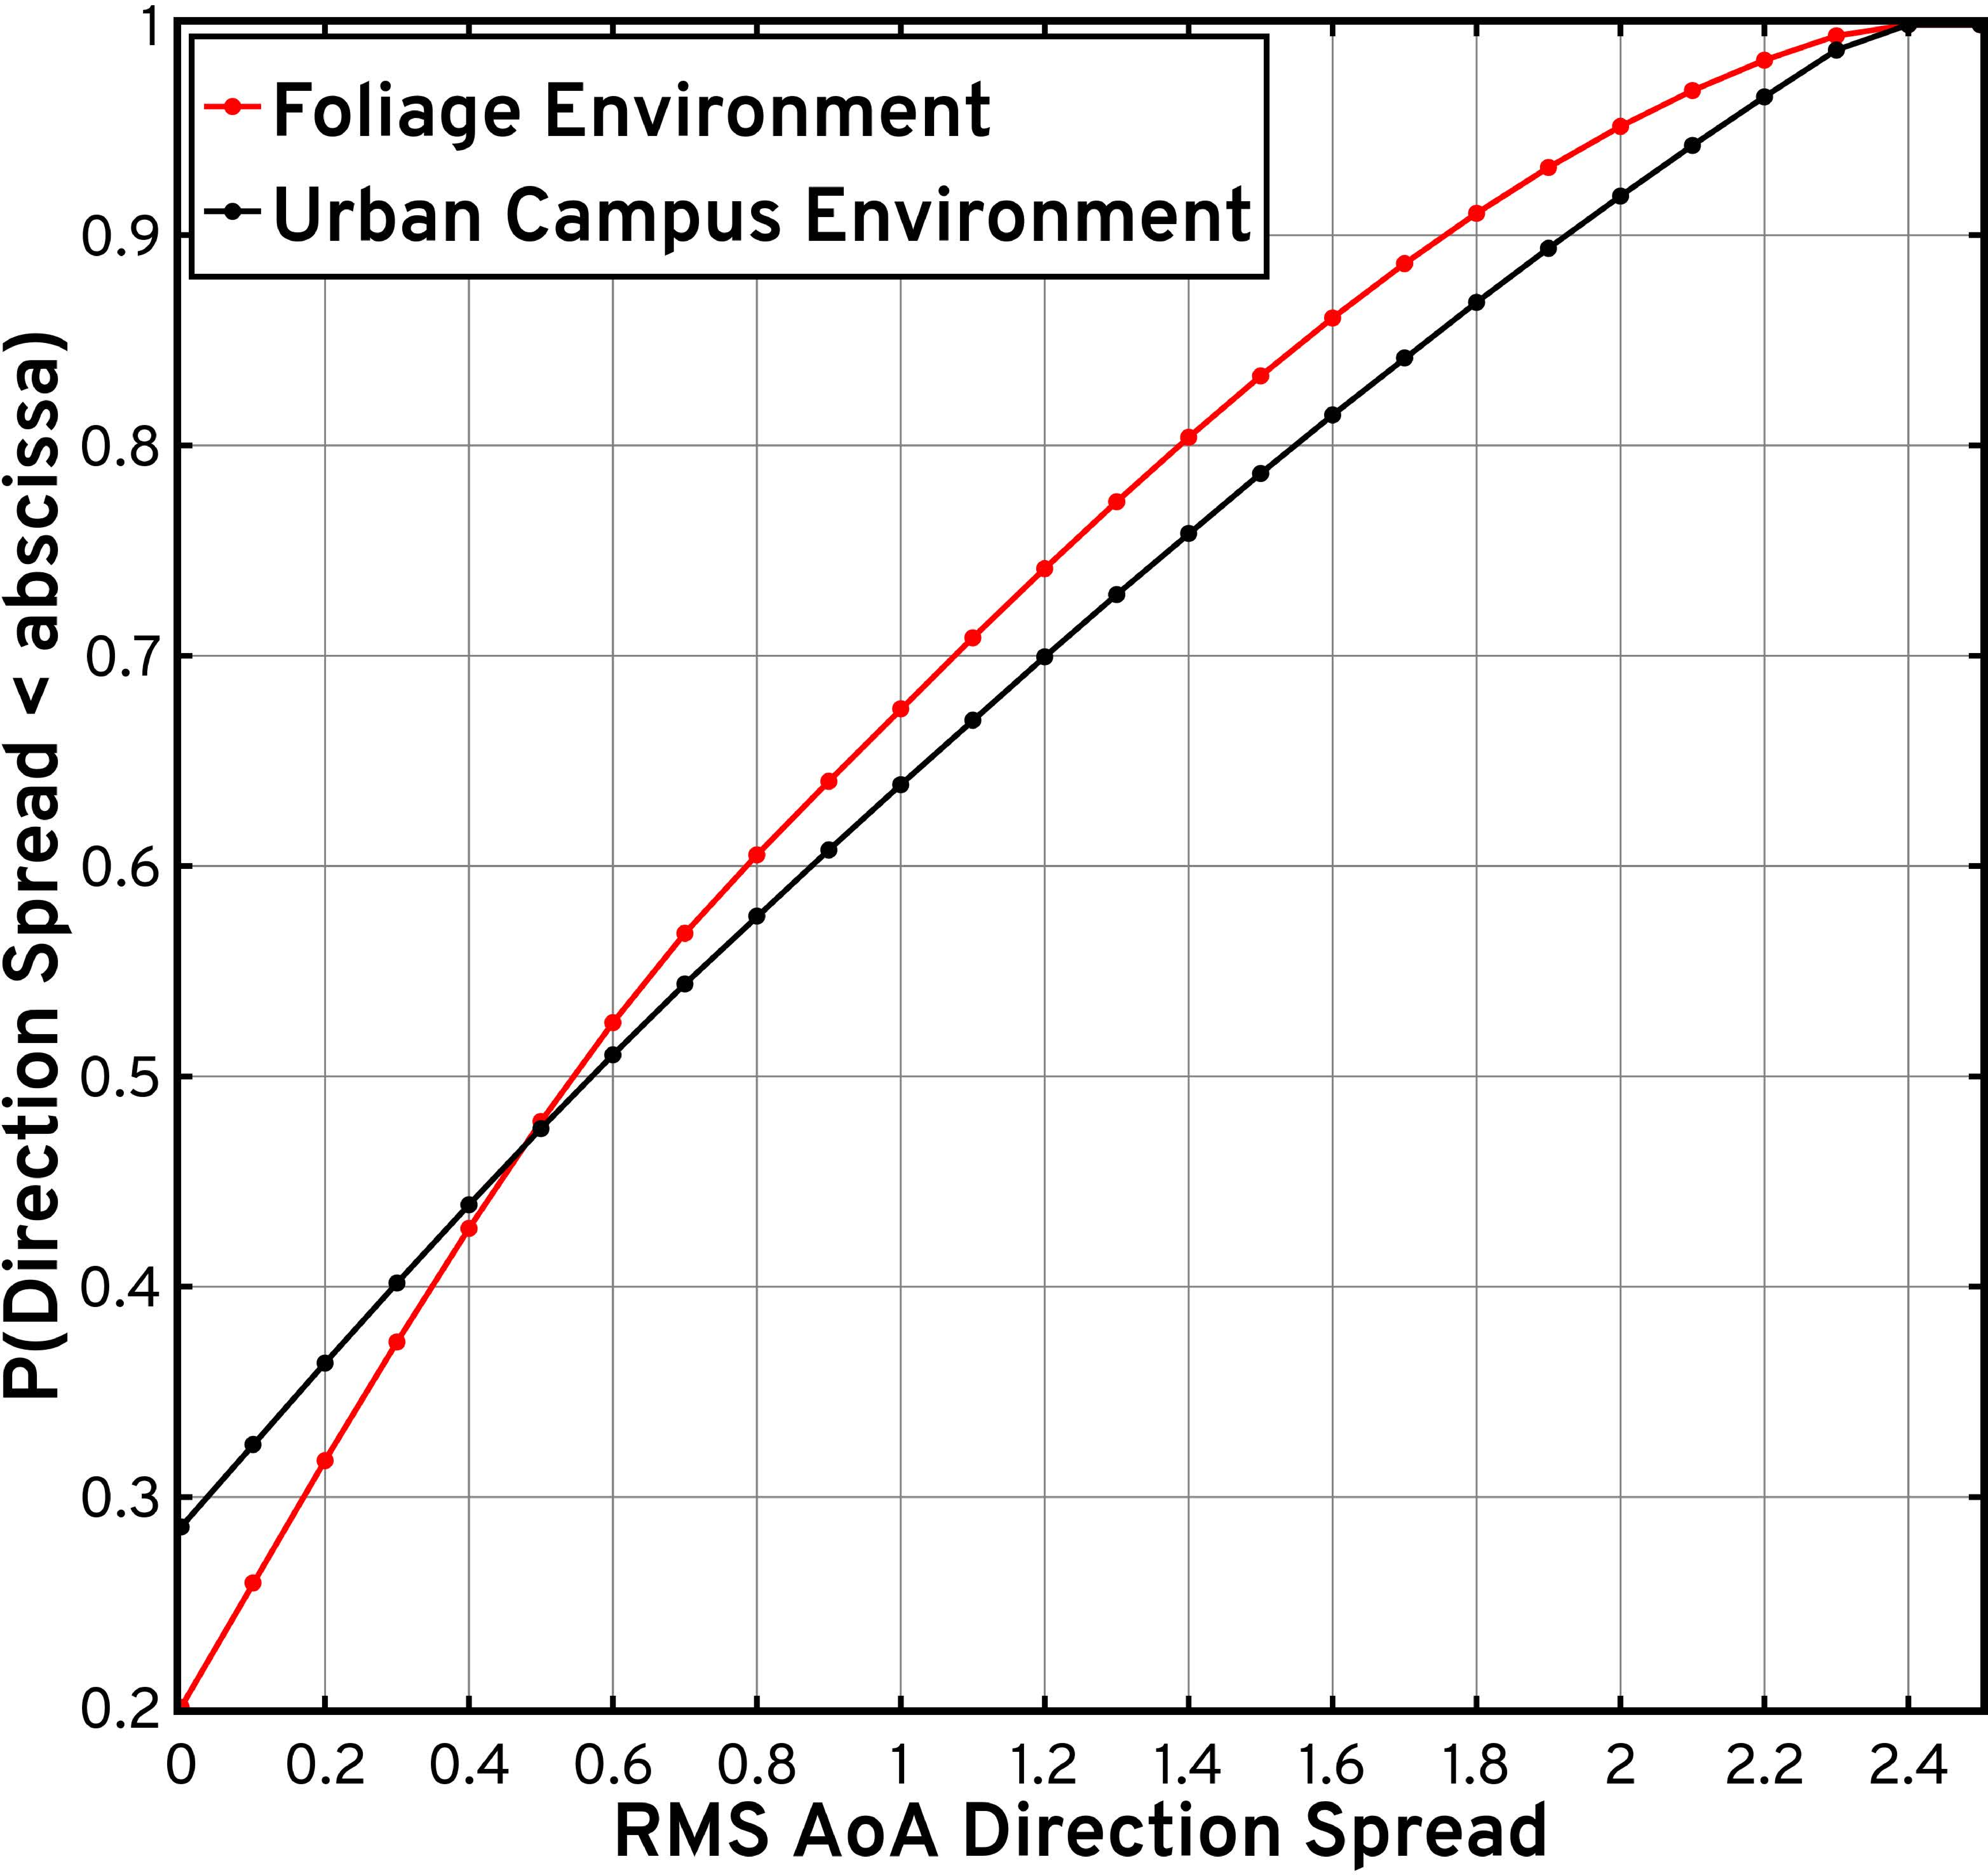
\includegraphics[width=1.0\linewidth]{figs/rms_direction_spread.pdf}
        \caption{RMS AoA Direction-Spread CDFs}
        \label{F11b}
    \end{subfigure}
    \vspace{-8mm}
    \caption{The plots depicting the CDFs of the RMS delay-spreads (a) and the RMS AoA direction-spreads (b) obtained from our measurements along various routes onsite, i.e., the urban campus route around $100$ S St (Rx is on a push-cart), the suburban neighborhood route around S Wolcott St (Rx is on a push-cart), and the foliage-dominated route around the Olpin Union building (Rx is again on a push-cart). These plots also involve the CDFs derived from the SV~\cite{SV_Molisch}, QD~\cite{QDC_NIST}, and stochastic~\cite{Indoor60G} models.}
    \label{F11}
\end{figure*}

Fig.~\ref{F11a} illustrates the RMS delay-spread characteristics of \SI{28}{\giga\hertz} signals, when the Tx is affixed atop the William Browning building and the Rx traverses unplanned vehicular routes around the urban campus, suburban neighborhood, and foliage environments. Herein, the RMS delay-spread metric is computed according to the following relationship (obtained from~\cite{Indoor60G})
\begin{align}\label{RMS_DS}
    \sigma_{\tau} = \sqrt{\frac{\sum_{\tau}P_{h}(\tau)\tau^{2}}{\sum_{\tau}P_{h}(\tau)} - \left(\frac{\sum_{\tau}P_{h}(\tau)\tau}{\sum_{\tau}P_{h}(\tau)}\right)^{2}},
\end{align}
where $P_{h}(\tau)$ denotes the power-delay profile obtained from the channel impulse response $h(\tau)$, i.e., $P_{h}(\tau){=}|h(\tau)|^{2}$. Fig.~\ref{F11a} also illustrates the RMS delay-spread CDFs for the SV~\cite{SV_Molisch}, QD~\cite{QDC_NIST}, and stochastic~\cite{Indoor60G} mmWave channel models. Also, the Kolmogorov-Smirnov statistic $D_{n}{=}\sup_{x}|F_{n}(x){-}F(x)|$ quantifies the distance between the empirical CDF $F_{n}(x)$ obtained from $n$ independent and identically distributed measurement samples and the CDF of the reference distribution $F(x)$ (i.e., the RMS delay-spread CDFs derived from the statistical channel models); note that $x$ here corresponds to a metric under analysis in our evaluations (RMS delay- and direction-spreads, cluster inter-arrival times, and cluster decay attributes). Similarly, Fig.~\ref{F11b} depicts the RMS AoA direction-spread characteristics of \SI{28}{\giga\hertz} signals in our propagation modeling campaign onsite at the NSF POWDER experimental testbed, along unplanned Rx vehicular routes around the urban campus, suburban neighborhood, and foliage environments. The RMS AoA direction-spread metric is computed as follows (again, obtained from~\cite{Indoor60G})
\begin{align}\label{RMS_DirS}
    \sigma_{\Omega} = \sqrt{\sum_{l=1}^{L}|\mathbf{e}(\phi_{l}, \theta_{l}) - \boldsymbol{\mu}_{\Omega}|^{2}P(\phi_{l}, \theta_{l})},
\end{align}
where $l$ denotes the MPC index ($1$ to $L$), $\phi_{l}$ denotes the azimuth angle-of-arrival for the $l^{\mathrm{th}}$ MPC, $\theta_{l}$ denotes the elevation angle-of-arrival for the $l^{\mathrm{th}}$ MPC, and $P(\phi_{l}, \theta_{l})$ denotes the normalized power spectrum at $\phi_{l}$ and $\theta_{l}$ for the $l^{\mathrm{th}}$ MPC. Fig.~\ref{F11b} also illustrates the direction-spread CDFs for the SV~\cite{SV_Molisch}, QD~\cite{QDC_NIST}, and stochastic~\cite{Indoor60G} models. Furthermore, as is the case in our RMS delay-spread investigations, we evaluate the Kolmogorov-Smirnov statistic for the RMS AoA direction-spread wherein we calculate the aforementioned statistical distance between the empirical CDF of the RMS AoA direction-spread obtained from our measurements and the CDFs of the reference distributions outlined by the SV, QD, and stochastic mmWave channel models.
\begin{figure*} [t]
    \centering
    \begin{subfigure}{0.495\linewidth}
        \centering
        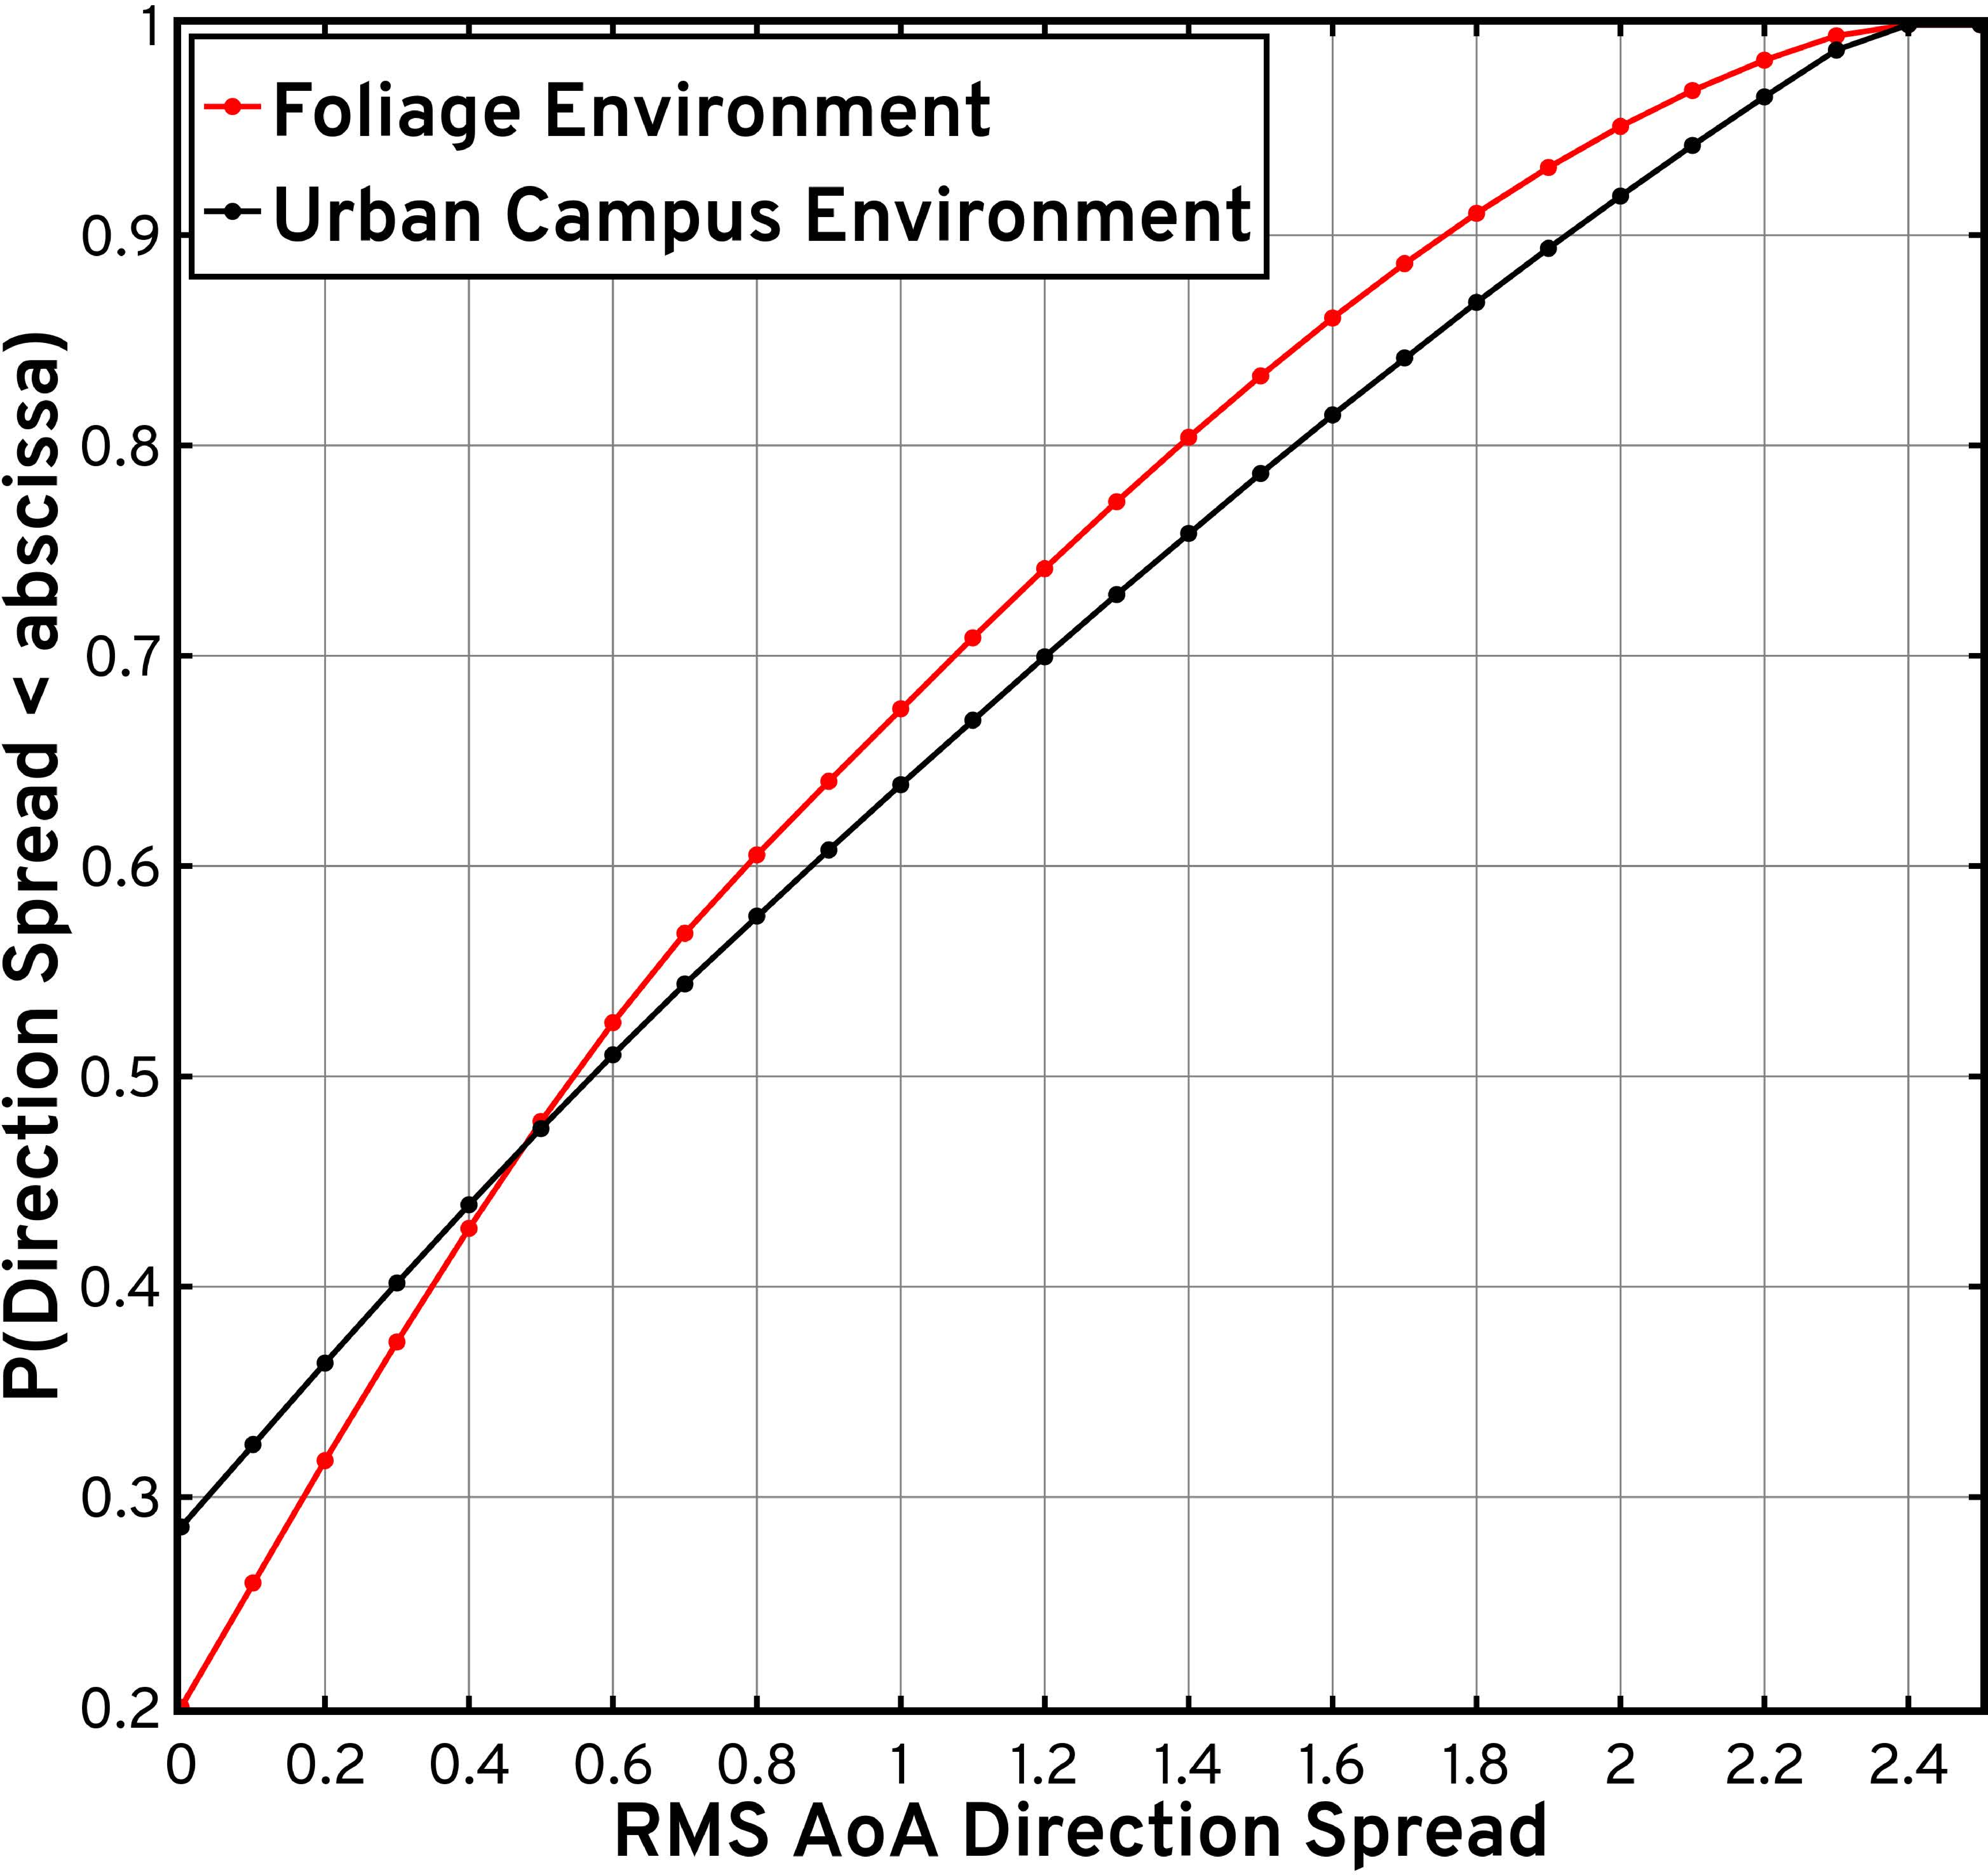
\includegraphics[width=1.0\linewidth]{figs/rms_direction_spread.pdf}
        \caption{Cluster Arrival Characteristics}
        \label{F12a}
    \end{subfigure}
    \begin{subfigure}{0.495\linewidth}
        \centering
        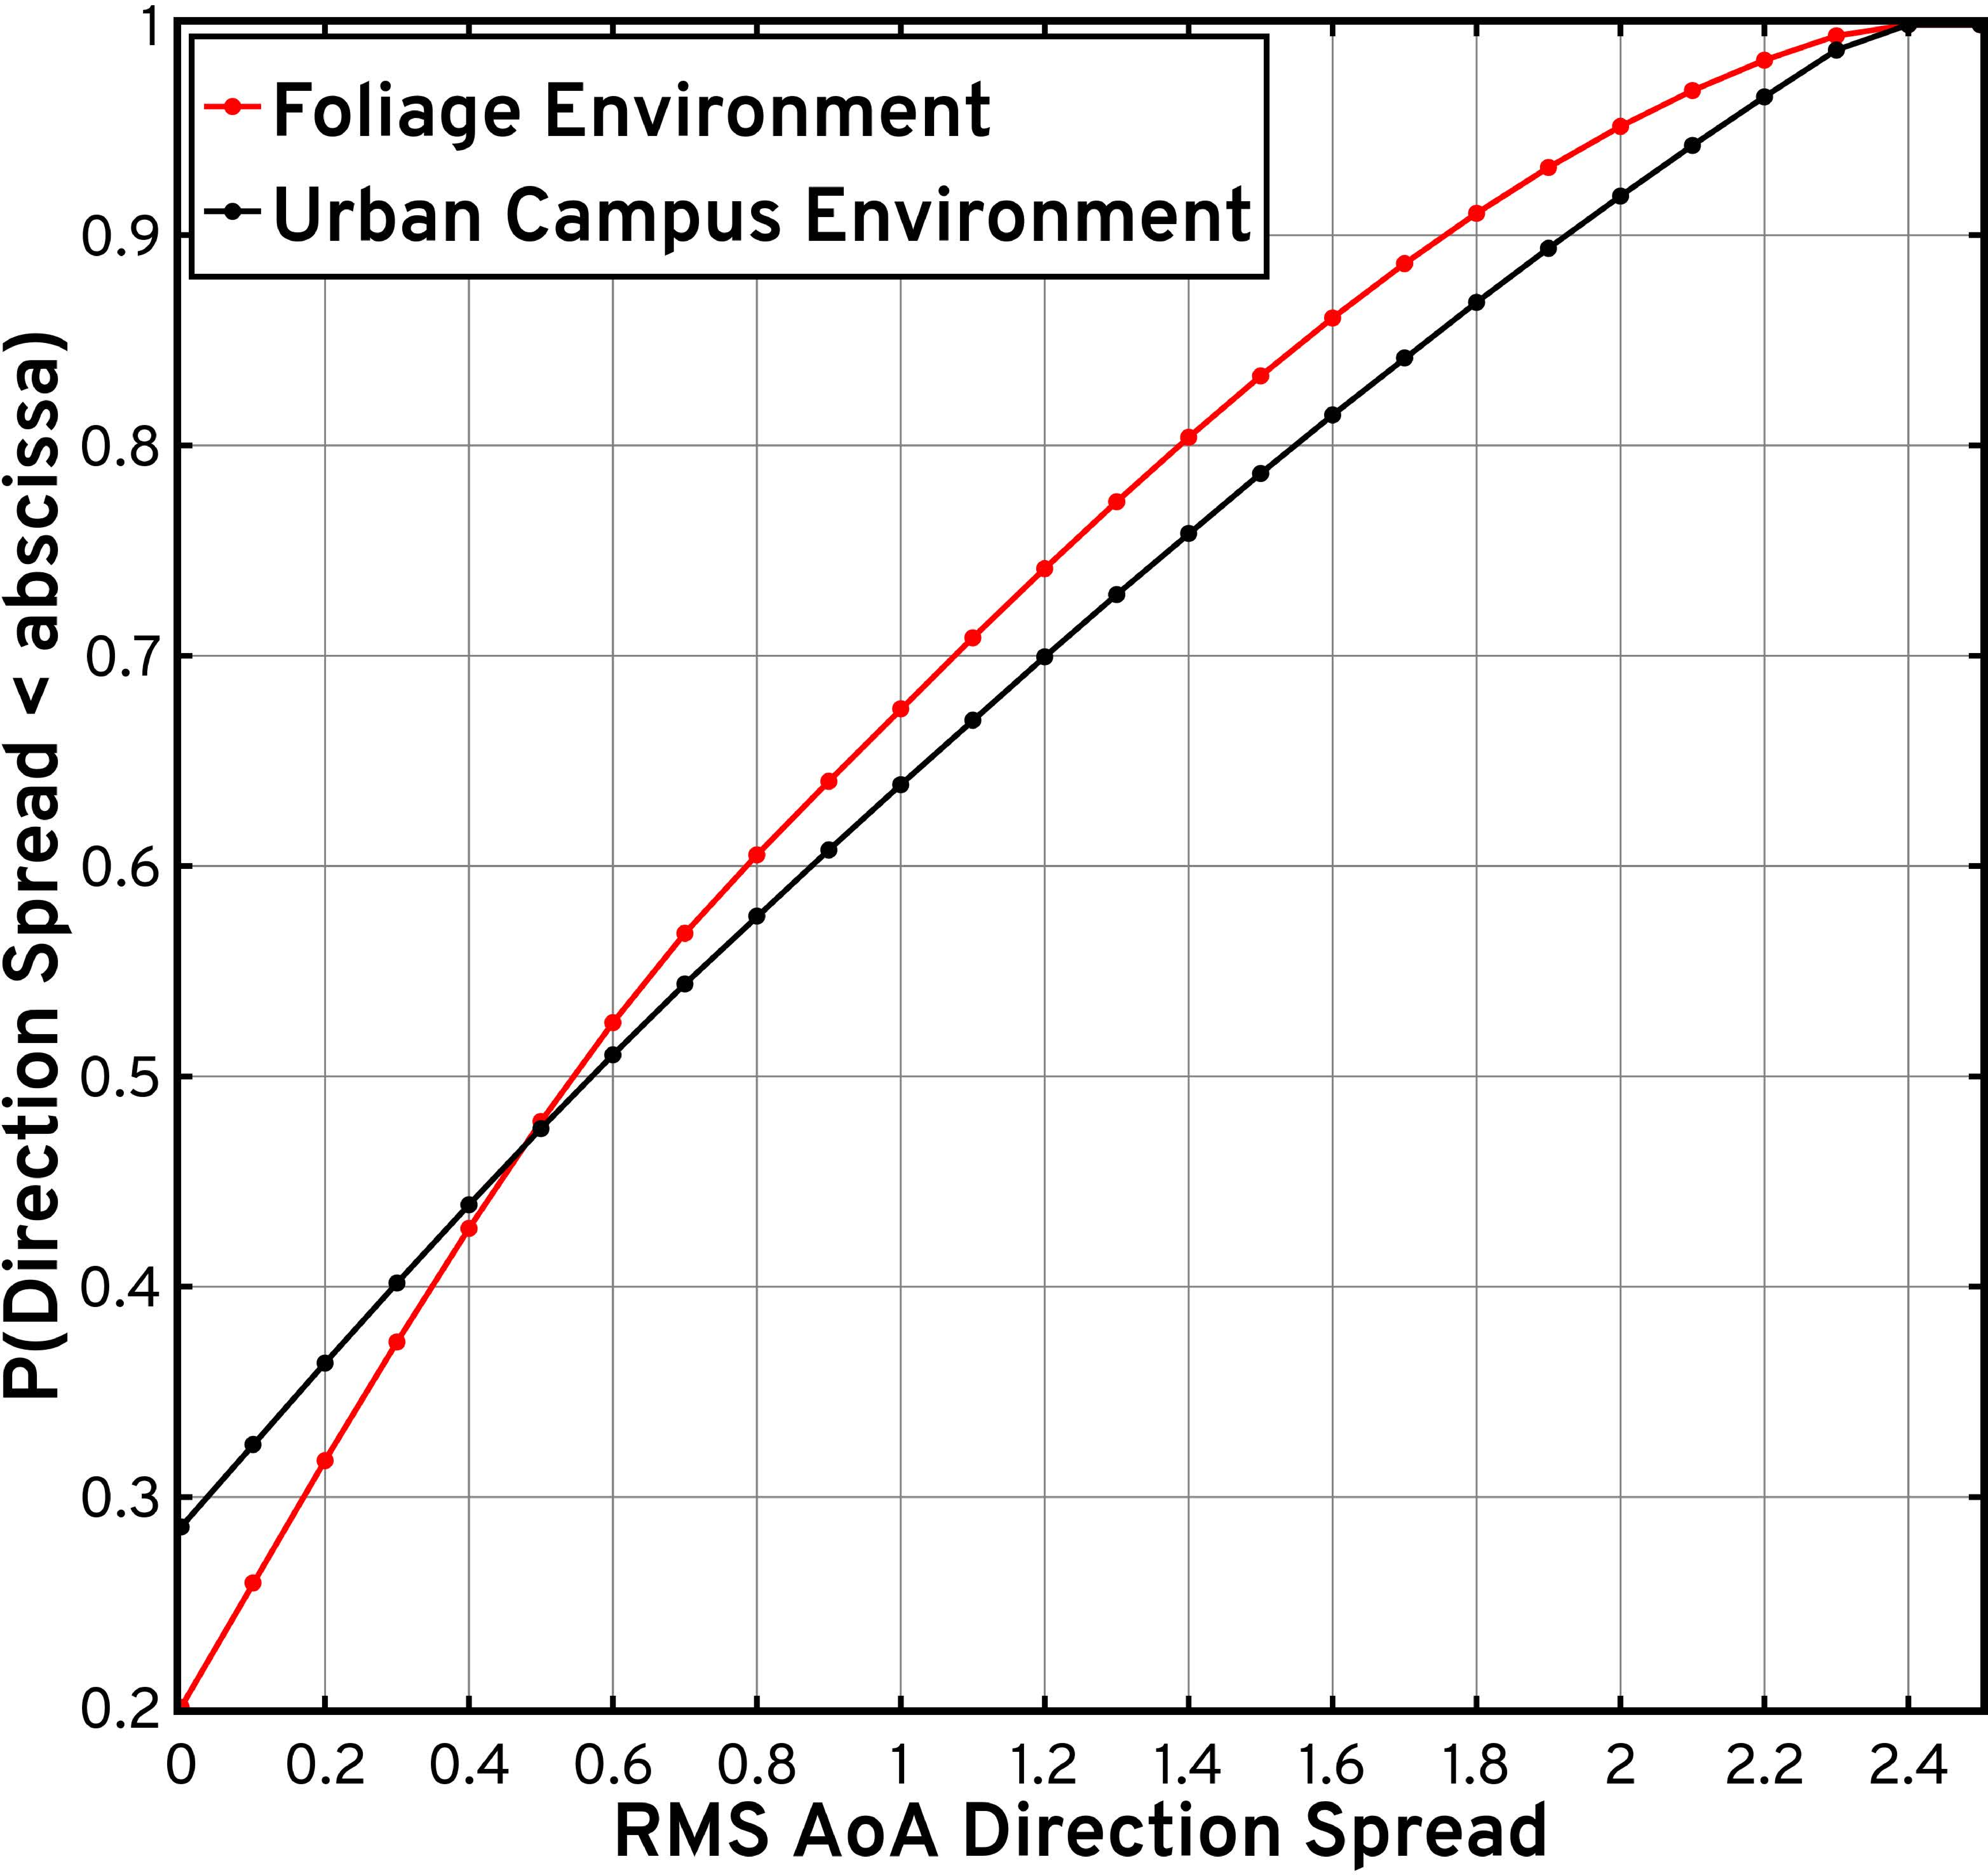
\includegraphics[width=1.0\linewidth]{figs/rms_direction_spread.pdf}
        \caption{Cluster Decay Characteristics}
        \label{F12b}
    \end{subfigure}
    \vspace{-8mm}
    \caption{The plots depicting the CDFs of cluster inter-arrival times (a) and cluster peak-power vs delay attributes (b) obtained from our measurements along various routes onsite, i.e., the urban campus route around $100$ S St (Rx is on a push-cart), the suburban neighborhood route around S Wolcott St (Rx is on a push-cart), and the foliage-dominated route around the Olpin Union building (Rx is again on a push-cart). The plots also show results from the SV~\cite{SV_Molisch}, QD~\cite{QDC_NIST}, and stochastic~\cite{Indoor60G} models.}
    \label{F12}
\end{figure*}

Finally, Fig.~\ref{F12a} illustrates the empirical CDF of the cluster inter-arrival times obtained from our onsite measurements at the NSF POWDER experimental testbed, with the Rx traversing unplanned routes around the urban campus, suburban neighborhood, and foliage environments. Furthermore, Fig.~\ref{F12a} depicts CDFs of the cluster inter-arrival times as detailed by the SV~\cite{SV_Molisch}, QD~\cite{QDC_NIST}, and stochastic~\cite{Indoor60G} channel models. Moreover, Fig.~\ref{F12b} depicts the empirical cluster decay characteristics (peak-power as a function of its absolute delay) of mmWave signals in V$2$X scenarios, in addition to a truncated regression curve-fitting model applied to these measurements~\cite{Indoor60G} along with empirical verifications against the statistical channel models.
\vspace{-3mm}

% Concluding remarks and Future work
\section{Conclusion}\label{S6}
In this work, we discuss the design of a fully-autonomous beam-steering platform coupled with a sliding-correlator channel sounder, well-suited for mmWave V$2$X modeling. Corroborated onsite, this beam-steering system demonstrates superior performance vis-\`{a}-vis geo-positioning accuracy, alignment reliability, and tracking response times. Processing the recorded power delay profiles via custom noise elimination and thresholding heuristics, we perform pathloss evaluations against the popular $3$GPP TR$38.901$, ITU-R M$.2135$, METIS, and mmMAGIC outdoor urban micro- and macro-cellular standards. Herein, we demonstrate that such standards particularly fail to accurately model the pathloss versus log-distance behavior of \SI{28}{\giga\hertz} signals in V$2$X networks within urban, suburban, and foliage environments. In addition to shadow-fading investigations, this paper reports (and compares against the D$2$D model) the small-scale fading properties of the obstructed signal, i.e. the average fade depth and duration, under dynamic blockages (pedestrians and moving/parked vehicles) in V$2$X scenarios. Crucially, the continuous series of measurements facilitated by our design enables signal decoherence studies under distance and alignment accuracy effects, wherein we demonstrate rapid decorrelation for minor distance and alignment changes. Finally, centered around the Kolmogorov-Smirnov statistic, multipath clustering analyses facilitate empirical validations of the SV, QD, and stochastic channel models vis-\`{a}-vis the cluster arrival \& decay characteristics and the RMS delay- \& direction-spreads.
\vspace{-3mm}

% References (main.bib)
\bibliographystyle{IEEEtran}
\bibliography{IEEEabrv,main}

\end{document}
% Content ends